\documentclass[twoside]{book}
\usepackage{book}
\usepackage{notations}
\usepackage{change}
    
\hypersetup{
pdftitle={Геометрия группы симплектоморфизмов},
pdfauthor={Л. В. Полтерович (Перевод с английского Р. Г. Матвеева и А. М. Петрунина
pод редакцией Л. В. Полтеровича и Я. М. Элиашберга)},
pdfsubject={Дифференциальная геометрия}}
 
%\geometry{a4paper,layoutsize={142mm,210mm},layoutoffset={3.5cm,4cm},marginparwidth=12em,hratio={1:1},vratio={3:4},width=110mm,height=172mm,ignorehead,ignorefoot,heightrounded}

\renewcommand\?[2]{#1}
\geometry{top=0.9in, bottom=0.85in,inner=0.9in, outer=0.7in, paperwidth=6in, paperheight=9in} %print

%\overfullrule=100mm

\begin{document}
%\pagestyle{empty}


\title{Геометрия группы симплектоморфизмов}
\author{Л. В. Полтерович
\\
\\
Перевод с английского
\\
Р. Г. Матвеева и А. М. Петрунина.
\\
\\
Под редакцией\\
Л. В. Полтеровича и Я. М. Элиашберга.
}
\date{}
\maketitle

\thispagestyle{empty}
\noindent\textbf{Л. В. Полтерович}

Геометрия группы симплектоморфизмов/
пер. с англ. Р. Г. Матвеева и А. М. Петрунина;
под ред. Л. В. Полтеровича и Я. М. Элиашберга.

\

Предварительное издание предназначенное исключительно для отлова ляпов. 
Исправления слать по адресу 
\url{petrunin@math.psu.edu}
или
\url{matveev@mis.mpg.de}.
\null
\vfill
Translation from the English language edition:
The Geometry of the Group of Symplectic Diffeomorphisms by Leonid Polterovich
\\
Copyright \textcopyright{} Birkhäuser Verlag AG, 2001.
All Rights Reserved.
\vfill
\noindent{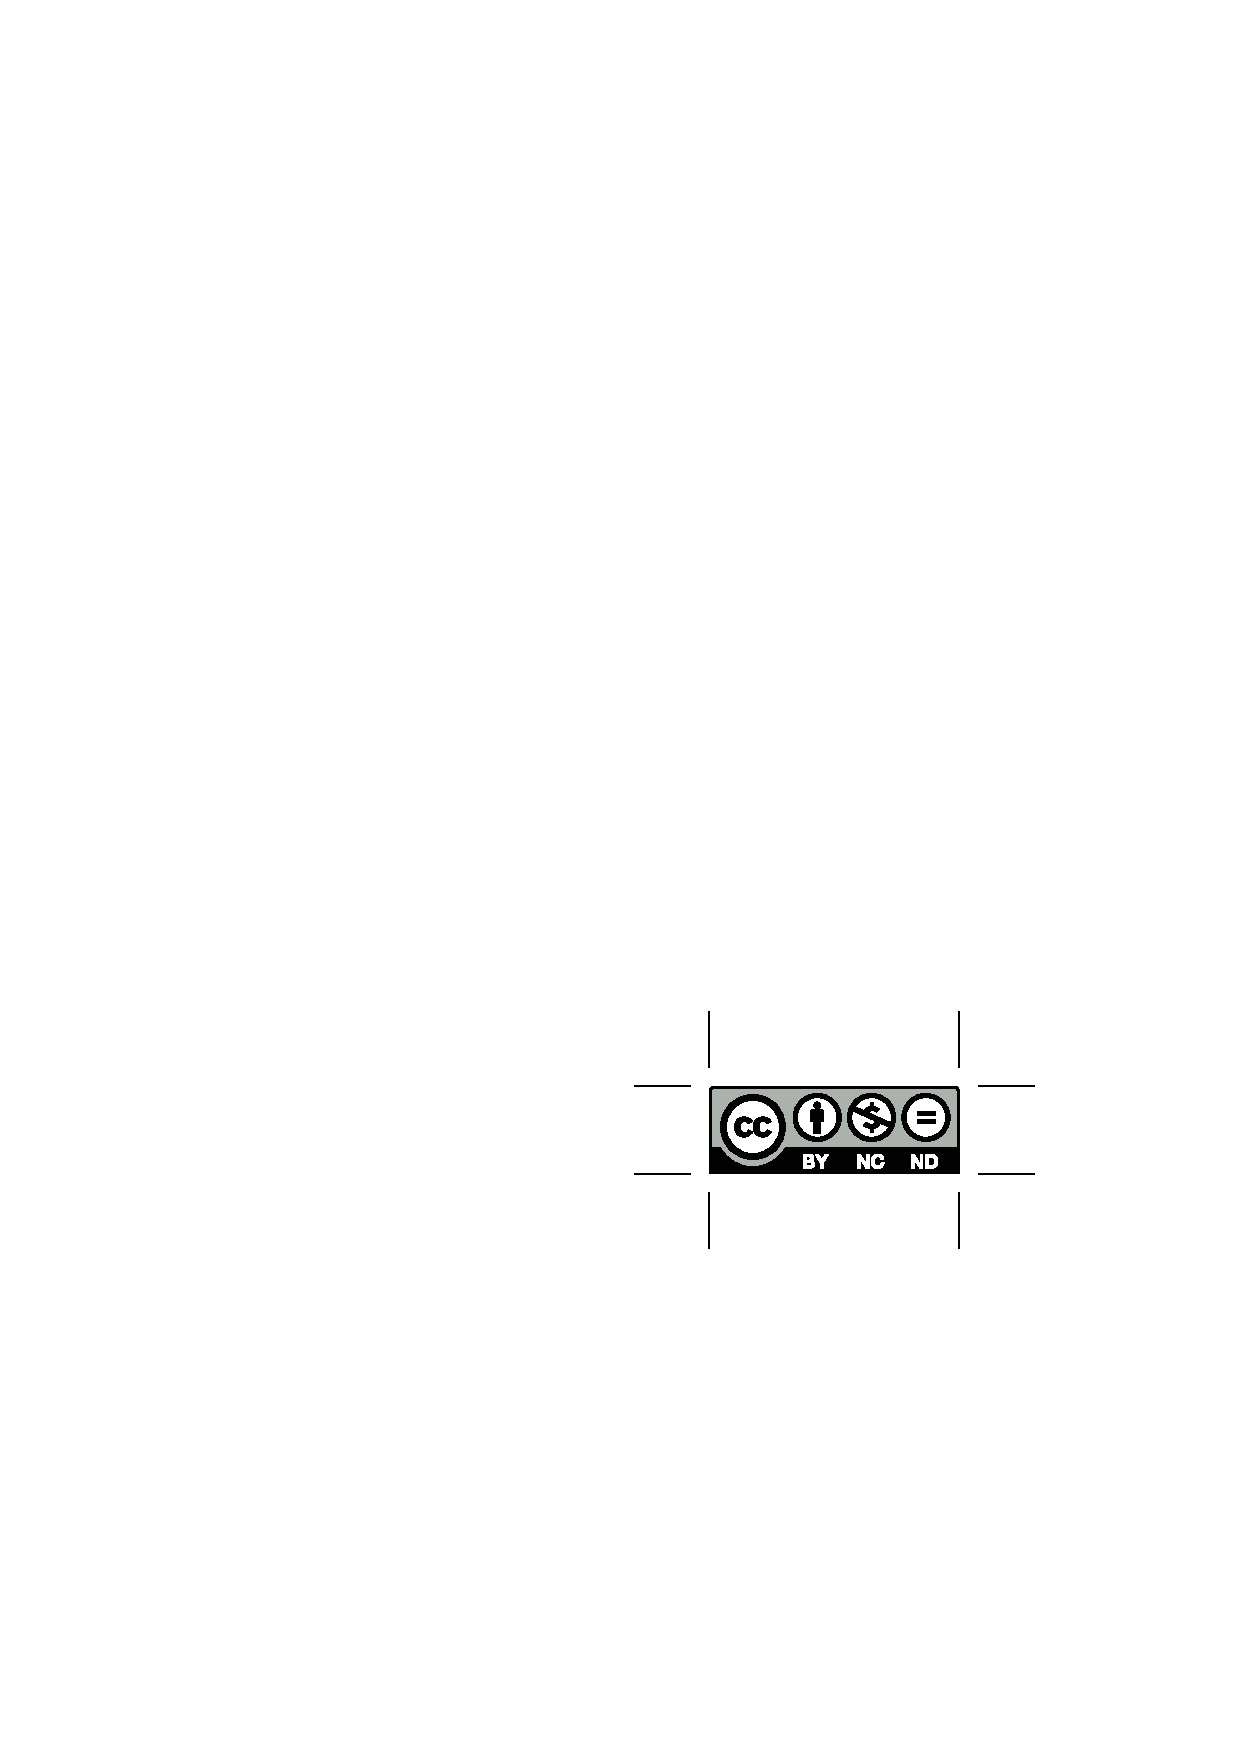
\includegraphics[scale=0.5]{pics/by-nc-nd}
\vspace*{1mm}
\\
\hbox{\parbox{1\textwidth}
{Лицензия: CC BY-NC-ND 4.0,\\
\texttt{https://creativecommons.org/licenses/by-nc-nd/4.0/}}}


\tableofcontents
\chapter*{Предисловие}

Группа гамильтоновых диффеоморфизмов $\Ham(M,\Omega)$ симплектического
многообразия $(M,\Omega)$ играет
основополагающую роль в геометрии и
механике.  Для геометра, по крайней мере при некоторых предположениях
о многообразии $M$, это связная компонента тождественного отображения
в группе всех симплектических диффеоморфизмов.  С точки зрения
механики, $\Ham(M,\Omega)$ является группой всех допустимых движений.
Какое минимальное количество энергии, необходимо для реализации
данного гамильтонова диффеоморфизма $f$?  Попытка формализовать этот
естественный вопрос и ответить на него привёл Х. Хофера \cite{H1}
(1990) к удивительному открытию.  Оказалось, что решение этой
вариационной задачи можно интерпретировать как \emph{геометрическую
  величину}, а именно как расстояние между $f$ и тождественным
отображением.  Кроме того, это расстояние связано с \?{канонической
  биинвариантной метрикой}{это что? не пытался ли Лёня сказать, что
  хоферовская метрика и есть та самая биинвариантная метрика? Думаю,
  да, но лучше спросить.} на $\Ham(M,\Omega)$.  Начиная с работ
Хофера, эта новая геометрия интенсивно изучалась в рамках современной
симплектической топологии.  В настоящей книге я опишу кое-что из
полученых результатов.

Хоферовская геометрия позволяет изучать различные понятия и задачи из знакомой нам конечномерной геометрии в контексте группы гамильтоновых диффеоморфизмов.
При этом они сильно отличаются от обычного круга задач, рассматриваемых в симплектической топологии и, таким образом, значительно расширяют \change{наше видение симплектического мира}{наши горизонты в симплектическом мире}.
Бесконечен ли диаметр $\Ham(M,\Omega)$?
Какие там кратчайшие?
Как найти спектр длин?
В общем случае, эти вопросы остаются открытыми.
Однако некоторые частные ответы существуют и будут нами рассмотрены.

Есть ещё одна, на мой взгляд, даже более важная причина, почему полезно иметь каноническую геометрию на группе гамильтониановых диффеоморфизмы.
Рассмотрим зависящее от времени векторное поле $\xi_t$, $t\in \RR$ на многообразии $M$.
Обыкновенное дифференциальное уравнение
\[\dot x=\xi(x,t)\]
на $M$ определяет поток $f_t\: M \to M$, который отображает точку $x(0)$ в $x(t)$ --- значение решения в момент времени $t$.
Траектории потока образуют сложную систему кривых на многообразии.
Обычно для того, чтобы разобраться в динамике, нужно следить за этими кривым на многообразии и изучить их поведение в разных регионах.
Сменив точку зрения мы видим, что наш поток становится простым
геометрическим объектом --- одной кривой $t \mapsto f_t$ на группе всех диффеоморфизмов многообразия.
Хочется надеяться, что геометрические свойства этой кривой отражают динамику и, в таком случае, сложную динамику можно изучать чисто геометрическими средствами.
Разумеется за это придётся платить.
Дело в том, что объемлющее пространство --- группа
диффеоморфизмов --- бесконечномерно.
Более того, встаёт другая серьёзная проблема:
в общем случае у нас нет канонических инструментов для выполнения геометрических измерений по этой группе.
Примечательно, что хоферовская метрика даёт такой инструмент для систем классической механики.
В главах 8 и 11 мы рассмотрим некоторые ситуации,
когда такой ход рассуждений оказывается полезным.

Как это часто случается с молодыми быстроразвивающимися областями математики, доказательства некоторых красивых утверждений хоферовской геометрии оказываются технически сложными.
Поэтому я выбирал самые простые нетривиальные случаи основных утверждений (на свой вкус, конечно), не пытаясь представить их в максимально возможной общности.
По той же причине опущены многие технические детали.
Хотя формально эта книга не требует специальных знаний в симплектической топологии (по крайней мере, необходимые определения и формулировки приведены), я рекомендую читателю  два замечательных вводных текста \cite{HZ} и \cite{MS}.
Оба содержат главы по геометрии группы гамильтониановых диффеоморфизмов.
Я постарался избежать повторов.
Книга содержит упражнения, которые предположительно помогут читателю вникнуть в предмет.

Эта книга возникла из двух источников.
Первый --- это лекции для аспирантов, а именно миникурсы в университетах Фрайбурга и Уорика, а также курс лекций в Швейцарской высшей технической школе Цюриха.
Вторым источником является обзорная статья \cite{P8}, которая содержит
вкратце материал приведённый ниже.

Теперь я коротко опишу содержание книги.
Дифффеоморфизм $f$ симплектического многообразия $(M,\Omega)$
называется гамильтоновым если его можно включить в гамильтонов поток
$f_t$ с компактным носителем удовлетворяющий $f_0=\1$ и $f_1 =f$.
Такой поток определяется гамильтонианом $F\: M \times [0, 1] \to \RR$.
На языке классической механики, $F$ --- энергия механического движения, описывающая $f_t$.
Мы понимаем полную энергию потока как длину соответствующего пути диффеоморфизмов:\?{}{добавил скобки под интеграл}
\[\length \{f_t\} =
\int_0^1\left(\max_{x\in M}F(x,t)-\min_{x\in M}F(x,t)\right) dt 
\]%добавил скобки
Определим функцию
\[\rho\: \Ham(M,\Omega) \times \Ham(M,\Omega) \to \RR\]
как
\[\rho (\phi, \psi) = \inf \length \{f_t\},\]
где точная нижняя грань берётся по всем гамильтоновым потокам $\{f_t\}$, которые
порождают гамильтонов диффеоморфизм $f = \phi\psi^{-1}$.
Легко видеть, что $\rho$ неотрицательна, симметрична, обращается в ноль на диагонали и удовлетворяет неравенству треугольника.
Более того, $\rho$ биинвариантно по отношению к групповой структуре на $\Ham(M,\Omega)$.
Другими словами, $\rho$ --- биинвариантная псевдометрика.
Глубокий факт состоит в том, что $\rho$ --- настоящая \?{метрика}{Вроде «метрика» больше подходит --- Лёня использует distance, но имеет в виду метрику --- функцию расстояния}, то есть $\rho (\phi, \psi)$ строго положительна при $\phi \ne \psi$.
Метрика $\rho$ называется хоферовской метрикой.

Группа $\Ham(M,\Omega)$ и хоферовская псевдометрика $\rho$ обсужадются в главах 1 и 2 соответственно.
В главе 3 доказывается, что $\rho$ является настоящей метрикой в случае, когда $M$ есть стандартное симплектическое линейное пространство $\RR^{2n}$.
Наш подход основан на теории Громова голоморфных дисков с Лагранжевыми граничными условиями, см.
главу~4.

Затем мы переходим к изучению основных геометрических инвариантов $\Ham(M,\Omega)$.
Существует (пока ещё открытая!) гипотеза о том, что диаметр $\Ham(M,\Omega)$ бесконечен.
В главах 5--7 эта гипотеза доказывается для замкнутых поверхностей.

В главе 8 обсуждается рост однопараметрической подгруппы $\{f_t\}$ группы $\Ham(M,\Omega)$, которая описывает асимптотическое поведение функции $\rho (\1, f_t)$ при $t \to \infty$.
Мы описываем связь между ростом и динамикой $\{f_t\}$ в контексте
теориии инвариантных торов классической механики.

Во многих интересных ситуациях пространство $\Ham(M,\Omega)$ имеет сложную топологию и, в частности, нетривиальную фундаментальную группу.
Для элемента $\gamma\in\pi_1(\Ham(M,\Omega))$ положим $\nu(\gamma) \z= \inf \length \{f_t\}$, где
точная нижняя грань берётся по всем петлям $\{f_t\}$ гамильтоновых
диффеоморфизмов (то есть, по периодическим гамильтоновым потокам),
которые представляют класс петель.
Множество
\[\set{\nu(\gamma)}{\gamma\in\pi_{1}\Ham(M,\Omega)}\]
называется спектром длин группы $\Ham(M,\Omega)$.
В главе 9 мы представляем подход к спектру длин, основанный на теории симплектических расслоений.
Важным компонентом этого подхода является теория Громова псевдоголоморфных кривых, обсуждаемая в главе~10.
В главе 11 приводятся приложения наших результатов к спектру длин в классической эргодической теории.

В главах 12 и 13 развиваются два разных подхода к теории геодезических на $\Ham(M,\Omega)$.
Один из них элементарный, а другой требует мощного инструмента --- гомологий Флоера.
Глава 13 предлагает читателю краткое введение в гомологии Флоера.

Наконец, в главе 14 мы имеем дело с негамильтоновыми симплектическими диффеоморфизмами, которые естественно появляются в хоферовской геометрии как изометрии $\Ham(M,\Omega)$.
Кроме того, мы формулируем и обсуждаем знаменитую \?{гипотезу о
  \red{симплектическом} потоке}{flux conjecture? Не нашли в русской литературе.}
заключающююся в том, что группа $\Ham(M,\Omega)$ замкнута в группе всех симплектических диффеоморфизмов, наделённой $C^\infty$-топологией. 

\paragraph*{Благодарности.}
Я сердечно благодарен \?{Мейке Аквельд}{Meike Akveld --- she+Swiss?} %
за её незаменимую помощь в напечатании предварительной версии рукописи,
подготовку рисунков и огромную редакционную работу.
Я очень благодарен \?{Паулю Бирану}{Paul Biran} и Карлу Фридриху Сибургу за их подробные комментарии к рукописи и за улучшение изложения.
Я признателен \?{Рами Айзенбуду}{Rami Aizenbud}, Диме Гуревичу, Мише Энтову, Осе Полтерович и Зеэву Руднику за указание на ряд неточностей в предварительной версии книги.
Книга была написана во время моего пребывания в Швейцарской высшей технической школе Цюриха в 1997--1998 учебном году и во время моих визитов в Институт высших научных исследований, Бюр-сюр-Иветт в 1998 и 1999 годах.
Я благодарю оба этих института за прекрасную исследовательскую атмосферу. 

\chapter*{Предисловие автора к русскому переводу}
%% The past two decades had brought a number of inter-
%% esting developments in Hofer’s geometry on groups of Hamiltonian diffeomor-
%% phisms. For reader’s convenience, I added a couple of comments, including up-
%% to-date bibliographical references, on several obsolete remarks and resolved
%% problems and/or conjectures.
За последние два десятилетия хоферовская геометрия группы
гамильтоновых диффеоморфизмов обогатилась рядом новых интересных
достижений.
Для удобства читателя я добавил к переводу несколько замечаний
вдобавок к уже устаревшим, а так же касающихся проблем и гипотез, для
которых были найдены решения. Кроме того, мною была добавлены ссылки на
несколько вновь появившихся публикаций.

\chapter{Знакомство с группой}\label{chap:1}

В этой главе мы пройдёмся по некоторым хорошо известным фактам касающихся группы гамильтоновых диффеоморфизмов.

\section[Гамильтоновы диффеоморфизмы]{Гамильтоновы диффеоморфизмы}

Рассмотрим движение частицы массы 1 в $\RR^n(q)$, где $q$ обозначает координату\footnote{Здесь и далее  $q$ это сокращённая запись для $q_1,\dots,q_n$. --- \textit{Прим. ред.}} в $\RR^n$, под действием потенциальной силы $\Phi(q, t)  \z= - \tfrac{\partial U}{\partial q} (q, t)$.
Соглачно второму закону Ньютона, $\ddot q= \Phi (q, t)$.
За исключением некоторых редких случаев, это уравнение явно не решить.
Однако можно понять некоторые качественные свойства его решений.

Теперь применим небольшую хитрость.
Введём вспомогательную переменную $p = \dot q$, и рассмотрим функцию $F(p,q,t)= \tfrac {p^2} 2 + U (q, t)$.
Функция $F$ представляет собой полную энергию частицы (сумму её кинетической и потенциальной энергий).
В этих обозначениях приведённое выше уравнение Ньютона можно переписать следующим образом:
\[
\begin{cases}
\quad\dot p &= - \tfrac{\partial F}{\partial q} (p, q, t),\\
\quad\dot q &= \tfrac{\partial F}{\partial p} (p, q, t).
\end{cases}
\]
Эта система дифференциальных уравнений первого порядка называется \rindex{гамильтонова система}\emph{гамильтоновой системой}.
Её следует рассматривать как обыкновенное дифференциальное уравнение в $2n$-мерном пространстве $\RR^{2n}$ с координатами $p$ и $q$.
Первый шаг любого исследования качественных свойств состоит в том, что надо отказаться думать о явной форме интересующего нас объекта.
Приняв это к сведению, давайте оставим в стороне выражение для функции
$F$ приведённое выше
и сосредоточимся на общем случае гамильтоновых систем, связанных с более-менее произвольными гладкими функциями энергии $F (p, q, t)$.
«Более-менее» означает, что мы накладываем определенные ограничения на поведение $F$ на бесконечности, гарантирующие то, что решения гамильтоновой системы существуют при всех $t\in \RR$.
Итак, выберем такое $F$ и рассмотрим поток $f_t\: \RR^{2n} \to \RR^{2n}$, переводящий любое начальное условие $\big(p(0),q(0)\big))$ в соответствующее решение $\big(p (t), q (t)\big)$ в момент времени $t$.
Возникающие таким образом диффеоморфизмы $f_t$ будут неформально называться \rindex{механическое движение}\emph{механическими движениями}.
Преимущество такого подхода состоит в том, что эти диффеоморфизмы $2n$-мерного пространства $\RR^{2n}$ обладают следующими замечательными геометрическими свойствами, которые не увидеть в исходном конфигурационном пространстве $\RR^n$.

\begin{thm}[(Теорема Лиувилля)]{Теорема}\label{1.1.A}\rindex{теорема Лиувилля}
Механические движения сохраняют форму объёма 
$\Vol=dp_1\wedge dq_1\wedge\dots\wedge d p_n\wedge dq_n$
\end{thm}

\begin{thm}[(Более тонкий вариант \ref{1.1.A})]{Теорема}\label{1.1.B}
Механические движения сохраняют 2-форму \?{}{Моет испарвить $\omega$ на $\Omega$ везде где можно?}$\omega = dp_1 \wedge dq_1 +\dots
+ dp_n \wedge dq_n.$
\end{thm}

Обратите внимание, что $\Vol = \tfrac{\omega^n}{n!}$ и значит, \ref{1.1.A} влечёт \ref{1.1.B}.
Далее, заметим, что при $n = 1$ теоремы \ref{1.1.A} и \ref{1.1.B} равносильны.
Теорема \ref{1.1.B} является простым следствием того факта, что механические движения происходят из гамильтоновой системы.
Мы приведём доказательство в следующем разделе.

Оба приведённых выше результата получены давно.
Сохранение объёма механическими движениями привлекало большое внимание уже более века назад.
Это послужило основной движущей силой при создании {}\emph{эргодической теории}, ныне хорошо известной математической дисциплины, изучающей различные свойства повторяемости преобразований, сохраняющих меру.
Однако значение роли инвариантной 2-формы $\omega$ было замечено сравнительно недавно.
Насколько я знаю, это был \rindex{Арнольд}В. И. Арнольд, он впервые прямо указал на это в 1960-х годах.
Попытки понять разницу между механическими движениями и диффеоморфизмами сохраняющими объём породила {}\emph{симплектическую топологию}, которая исследует неожиданные явления жёсткости, возникающие в теории симплектических многообразий и их морфизмов.

Вот пример такого явления, которое обнаружил \rindex{Сикорав}Дж. -C. Сикорав \cite{S1}.
Пусть $B^2(r) \subset \RR^2$ --- евклидов диск радиуса $r$, ограниченный окружностью $S^1(r)$.
Рассмотрим тор 
\[L_R = 
S^1 (R) \times\dots\times S^1(R) \subset \RR^2 (p_1, q_1) \times\dots\times \RR^2 (p_n, q_n) =\RR^{2n} (p, q)\]
и цилиндр $C_r = B^2 (r) \times \RR^{2n-2}$.

\begin{thm}[(Свойство несжимаемости)]{Теорема}\label{1.1.C}
Не существует механического движения, переводящего $L_R$ в $C_r$, при условии, что $R>r$.
\end{thm}

Мы докажем это утверждение в более общем виде в разделе \ref{3.2.A} ниже.
Отметим, что при $n = 1$ результат очевиден.
Действительно, площадь, ограниченная $S^1 (R)$, больше, чем площадь $B^2 (r)$.
Таким образом, нельзя перевести $S^1(R)$ в $B^2(r)$ преобразованием, сохраняющим площадь.
Однако если $n \ge 2$, то $L_R$ --- подмногообразие коразмерности $n \ge 2$, а $C_r$ имеет бесконечный объем.
Таким образом, нет видимой причины, по которой это утверждение должно быть верным.
Более того, подобное утверждение совершенно неверно в категории диффеоморфизмов сохраняющих объём!


\begin{ex*}{Упражнение}
Найти линейное преобразование $\RR^{2n} \to \RR^{2n}$, сохраняющее объём и переводящее $L_R$ в $C_r$ при произвольных положительных $r$ и $R$.
\end{ex*}

В дальнейшем эволюция механической системы будет рассматриваться как кривая в группе всех механических движений и эта кривая будет изучаться геометрическими средствами.
Чтобы всё работало, нам придётся сузить класс механических систем.
Например, неограниченные гамильтонианы, такие как $F(p,q,t) = \tfrac {p^2}2 + U(q,t)$ рассматриваемые выше, для нас будут слишком сложны.
Мы всегда будем предполагать, что гамильтонианы (и, следовательно, соответствующие им механические движения) имеют компактный носитель.
Другими словами, всё движение происходит в ограниченной части нашего пространства.

В этой главе вводится гамильтонова механика на симплектических многообразиях, которая является естественным обобщением модели, описанной выше.
Соответственно, гамильтонов диффеоморфизм --- это просто механическое движение, порождённое гамильтонианом с компактным носителем. 

\section{Потоки и пути диффеоморфизмов}

Для начала объясним связь между потоками и дифференциальными уравнениями и дадим геометрическую интерпретацию потоков как путей диффеоморфизмов.
Имея в виду будущие приложениями мы предполагаем, что все рассматриваемые нами объекты имеют компактный носитель.
Однако основные построения, описанные ниже, проходят в более общем случае.

Рассмотрим гладкое многообразие $M$ без края.
Пусть $\phi\: M \to M$ --- диффеоморфизм, определим его \rindex{носитель}\emph{носитель} \index[symb]{$\supp(\phi)$}$\supp(\phi)$ как замыкание всех  $x \in M$ таких, что $\phi(x) \ne x$.
Обозначим через $\Diff^c (M)$ группу всех диффеоморфизмов с компактным носителем.
Пусть $I \subset \RR$ --- интервал.%
\footnote{Мы определяем интервал как связное подмножество $\RR$ с непустой внутренней частью.}
\rindex{путь диффеоморфизмов}\emph{Путь диффеоморфизмов} --- это отображение 
\[f\: I \to \Diff^c (M),\quad t \mapsto f_t\]
со следующими свойствами:
\begin{itemize}
\item отображение $M \times I \to M$, переводящее $(x, t)$ в $f_t x$, гладкое;
\item существует компактное подмножество $K$ в $M$, содержащее $\supp f_t$ при всех $t \in I$.
\end{itemize}
Мы часто обозначаем такой путь через $\{f_t\}$.
Отметим, что на замкнутых многообразиях второе условие выполняется автоматически.

Каждый путь диффеоморфизмов порождает семейство векторных полей $\xi_t$, $t \in I$ на $M$ следующим образом: 
\begin{equation}\tfrac{d}{dt} f_t x = \xi_t (f_t x).
\label{eq:1.2.A}
\end{equation}
Отметим, что это семейство гладкое и имеет компактный носитель: $\xi_t (x) = 0$ при всех $x \in M \backslash K$.
Такое семейство называется \textit{зависящим от времени векторным полем с компактным носителем} на $M$.
Приведённое выше соответствие не является инъективным.
В самом деле, каждый путь вида $\{f_t g\}$, где $g$ --- произвольный элемент $\Diff^c (M)$, порождает то же самое зависящее от времени векторное поле $\xi$.
Однако для каждой точки $s \in I$ существует единственный путь $\{f_t\}$, который 
порождает $\xi$ такой, что $f_s$ равно тождественному отображению $\1$.
Этот путь определяется как единственное решение уравнения~(\ref{eq:1.2.A}), которое теперь рассматривается как обыкновенное дифференциальное уравнение с начальным условием $f_s = \1$.
Предположим, что $0 \in I$, и возьмём $s = 0$.
Построенный выше путь $\{f_t\}$ при $f_0 = \1$ называется \rindex{поток}\emph{потоком} зависящего от времени векторного поля $\xi$.
Таким образом, потоки --- это просто пути $\{f_t\}$, такие, что $f_0 = \1$.

\section[Классическая механика]{Математическая модель классической механики}

Роль фазового пространства в классической механике играет \rindex{симплектическое многообразие}\emph{симплектическое многообразие} $(M^{2n},\Omega)$.
Здесь $M$ --- связное многообразие без границы и имеющее чётную размерность $2n$, а $\Omega$ --- замкнутая дифференциальная 2-форма на $M$.
Форма $\Omega$ предпологается {}\emph{невырожденной}.
Это означает, что его максимальная степень $\Omega^n$ не обращается в нуль ни в какой точке.
Форма $\Vol =  \tfrac{\Omega^n}{n!}$ называется \rindex{объём}\rindex{форма объёма}\emph{канонической формой объёма} на $(M, \Omega)$.
Полезно иметь в виду два элементарных примера симплектических многообразий:
ориентируемую поверхность, наделённую формой площади, и линейное пространство $\RR^{2n} (p_1,\dots, p_n, q_1,\dots, q_n)$ с формой $\omega = \sum^n_{j = 1} dp_j \wedge dq_j$.
Второй пример очень важен с точки зрения классической \rindex{теорема Дарбу}\emph{теоремы Дарбу} \cite{MS}.
Она утверждает, что локально каждое симплектическое многообразие выглядит как $(\RR^{2n}, \omega)$.
Другими словами, для каждой точки $M$ можно выбрать такие локальные координаты $(p, q)$, что в этих координатах $\Omega$ записывается как $\sum^n_{j = 1} dp_j \wedge dq_j$.
Мы называем $(p, q)$ \rindex{канонические координаты}\emph{каноническими локальными координатами}.

Пусть $F$ --- гладкая функция на $M$.
Векторное поле $\xi$ на $M$ называется \rindex{гамильтоново векторное поле}\emph{гамильтоновым векторным полем} гамильтониана $F$, если оно поточечно удовлетворяет линейному алгебраическому уравнению $i_\xi \Omega \z= -dF$.
Элементарное рассуждение из линейной алгебры (основанное на невырожденности $\Omega$) даёт, что $\xi$ всегда существует и единственно \cite{MS}.
Иногда $\xi$ обозначают $\sgrad F$ (\rindex{косой градиент}\emph{косой градиент} $F$).

\begin{ex}{Упражнение}\label{1.3.A}
Докажите, что в канонических локальных координатах $(p, q)$ на
$M$ выполняется равенство \index[symb]{$\sgrad$} $\sgrad F = (-\tfrac{\partial F}{\partial q},\tfrac{\partial F}{\partial p})$
\end{ex}

\begin{ex}{Упражнение}\label{1.3.B}
Пусть  $\phi\: M \to M$ --- симплектический диффеоморфизм
(т. е. $\phi^\ast \Omega = \Omega$).
Докажите, что $\sgrad (F \circ \phi^{-1}) \z= \phi_\ast \sgrad F$ для любой функции $F$ на $M$.
Это свойство, конечно, отражает тот факт, что операция $\sgrad$ определяется бескординатным образом.
\end{ex}


В классической механике энергия определяет эволюцию системы.
Энергия -- это семейство функций $F_t$ на $M$, которое зависит от
дополнительного временного параметра $t$.
Время $t$ определено на некотором интервале $I$.
Эквивалентно, можно рассматривать энергию как одну единственную функцию $F$ на $M \times I$.
Мы будем использовать оба варианта на протяжении всей книги, сохраняя обозначение $F_t (x) = F (x, t)$.
Традиционно $F$ называется \rindex{гамильтониан}\emph{гамильтонианом (зависящим от времени)}.

Эволюция системы описывается \rindex{уравнение Гамильтона}\emph{уравнением Гамильтона} $\dot x \z= \sgrad F_t (x)$.
В локальных канонических координатах $(p, q)$ на $M$ уравнение
Гамильтона имеет знакомый вид (сравните с \ref{1.3.A})
\[
\begin{cases}
\quad\dot p &= - \tfrac{\partial F}{\partial q} (p, q, t),\\
\quad\dot q &= \tfrac{\partial F}{\partial p} (p, q, t).
\end{cases}
\]

Введём линейное функциональное пространство \index[symb]{$\A$}\index[symb]{$\A(M)$}$\A=\A(M)$, которое будет играть важную роль ниже.
Если $M$ замкнуто, определим $\A(M)$ как пространство всех гладких функций на $M$ с нулевым средним относительно канонической формы объёма.
Если $M$ открыто, то $\A(M)$ состоит из всех гладких функций с компактным носителем.

\begin{ex}{Определение}
Пусть $I \subset \RR$ --- интервал.
Гамильтониан $F$ (зависящий от времени) на $M \times I$ называется \rindex{нормализованный гамильтониан}\textbf{нормализованным}, если $F_t$ принадлежит $\A$ при всех $t$.
Если $M$ открыто, то мы дополнительно требуем, чтобы существовало компактное подмножество $M$, содержащее носители всех функций $F_t$, $t \in I$ одновременно.
\end{ex}

В дальнейшем будут рассматриваться только нормализованные гамильтонианы.
Приведём пару соображений в пользу этого соглашения.

Прежде всего, на открытых многообразиях необходимо наложить некоторые ограничения на поведение гамильтонианов на бесконечности.
В самом деле, в противном случае решения гамильтонова уравнения могут
убежать на бесконечность за конечное время и, таким образом, гамильтонов поток может быть плохо определен.
Важной особенностью приведенного выше определения является то, что зависящее от времени гамильтоново векторное поле $\sgrad F_t$ нормализованного гамильтониана $F$ имеет компактный носитель.
Таким образом, когда $I$ содержит $0$, такое поле определяет поток с компактным носителем, который вписывается в идеологию предыдущего раздела.

Во-вторых, как на открытых, так и на замкнутых многообразиях отображение, переводящее функцию из $\A$ в его гамильтоново векторное поле, инъективно.
Действительно, гамильтоново векторное поле определяет соответствующий гамильтониан однозначно с точностью до аддитивной константы.
Понятно, что наша нормализация запрещает добавлять константы!
Это свойство нормированных гамильтонианов будет полезно в дальнейшем.

\section[Группа гамильтоновых диффеоморфизмов]{Группа гамильтоновых\\диффеоморфизмов}\label{1.4}

Пусть $F: M \times I \to R$ --- нормализованный гамильтониан, зависящая от времени.
Предположим, что $I$ содержит ноль.
Рассмотрим поток $\{f_t\}$ зависящего от времени векторного поля $\sgrad F_t$.
Мы будем говорить, что $\{f_t\}$ --- \rindex{гамильтонов поток}\emph{гамильтонов поток}, порождённый $F$.
Каждый диффеоморфизм $f_a$, $a \in I$ этого потока называется \rindex{гамильтонов диффеоморфизм}\emph{гамильтоновым диффеоморфизмом}.
Из определения конечно следует, что гамильтоновы диффеоморфизмы имеют компактный носитель.

\begin{ex}[(репараметризация потоков)]{Упражнение}\label{1.4.A}
\rindex{параметризация потока}
Пусть $\{f_t\}, t \z\in [0; a]$ --- гамильтонов поток, порождённый нормированным гамильтонианом $ F (x, t)$.
Докажите, что $\{f_{at}\}$, $t \in [0; 1]$ тоже является гамильтоновым потоком, порождённым $aF (x, at)$.
Следовательно, любой гамильтонов диффеоморфизм на самом деле является отображением некоторого гамильтонова потока с единичным временем.
Более общо, покажите, что для любой гладкой функции $b (t)$ с $b (0) =
0$ поток $\{f_{b (t)}\}$ является гамильтоновым потоком, нормированный
гамильтониан которого равен $\tfrac{\d b}{\d t} (t) F (x, b (t))$.
\end{ex}

Ключевым свойством гамильтоновых диффеоморфизмов является то, что они сохраняют симплектическую форму $\Omega$.
В самом деле, пусть $\xi$ --- гамильтоново векторное поле функции $F$ на $M$.
Все, что нам нужно проверить, --- это равенство нулю производной Ли $L_\xi \Omega$.
Это видно из следующих вычислений: 
\[L_\xi \Omega = i_\xi \d\Omega + \d (i_\xi \Omega) = -\d\d F = 0.\]
Обозначим через \index[symb]{$\Ham (M, \Omega)$}$\Ham (M, \Omega)$ множество всех гамильтоновых диффеоморфизмов.

Путь диффеоморфизмов в $\Ham (M, \Omega)$ называется \rindex{гамильтонов путь}\emph{гамильтоновым путём}.
Естественно назвать поток со значениями в $\Ham (M, \Omega)$ гамильтоновым потоком.
Однако, немного подумав, мы понимаем, что попали в беду.
Действительно, гамильтоновы потоки уже были определены выше по-другому.
Заранее совсем не ясно, почему векторное поле, соответствующее гамильтонову пути, является гамильтоновым векторным полем!
К счастью, это правда.
Этот чрезвычайно важный факт был установлен \rindex{Баньяга}Баньягой \cite{B1}.
Вот его точная формулировка.

\begin{thm}{Предложение}\label{1.4.B}
Для каждого гамильтонова пути $\{f_t\}$, $t \z\in I$, существует (зависящий от времени) нормализованный гамильтониан $F\: M \times I \to \RR$ такой, что 
\[\tfrac \d{\d t} f_t x = \sgrad F_t (f_t x)\]
при всех $x \in M$ и $t \in I$.
\end{thm}

Функция $F$ называется нормализованным гамильтонианом
пути $\{f_t\}$.

Обсудим этот результат.
Сначала предположим, что многообразие $M$ удовлетворяет следующему
топологическому условию: его первая группа когомологий де Рама с компактными носителями равна нулю, то есть $H_{\mathrm{comp}}^1 (M, \RR) = 0$.
Чтобы иметь перед собой пример, представьте себе двумерную сферу или линейное пространство.
В этом случае приведённое выше предложение доказывается очень легко.
Обозначим через $\xi_t$ векторное поле, порождённое $f_t$.
Поскольку гамильтоновы диффеоморфизмы сохраняют симплектическую форму $\Omega$, имеем $L_{\xi_t} \Omega = 0$.
Следовательно, $\d i_{\xi_t} \Omega = 0$, поэтому $i_{\xi_t} \Omega$ --- замкнутая форма.
Ввиду нашего топологического условия форма $i_{\xi_t} \Omega$ точна.
Следовательно, существует единственное гладкое семейство функций $F_t (x) \in \A$ такое, что $-dF_t = i_{\xi_t} \Omega$.
Отсюда следует, что $F (x, t)$ --- нормированный гамильтониан $\{f_t\}$.
Это завершает доказательство.
Однако, когда $H^1_{\mathrm{comp}} (M, \RR) \ne 0$, нельзя  заранее знать, точны ли замкнутые формы $i_{\xi_t} \Omega$.
В этом случае следует дополнительно использовать то, что каждое отдельное $f_t$ гамильтоново.
Это требует некоторых новых идей, см. \cite{B1}, \cite{MS}.

\begin{ex}{Замечание}\label{1.4.C}
Пусть \index[symb]{$\Symp(M,\Omega)$}$\Symp(M,\Omega)$ --- группа всех диффеоморфизмов $f$ с компактным носителем на $M$, сохраняющих $\Omega$, то есть $f^\ast\Omega = \Omega$.
Такие диффеоморфизмы называются \rindex{симплектоморфизм}\emph{симплектоморфизмами}.
Обозначим через \index[symb]{$\Symp_0(M,\Omega)$}$\Symp_0(M,\Omega)$ компоненту линейной связности единицы в $\Symp(M,\Omega)$.
По определению она содержит те симплектоморфизмы $f$, которые можно соединить путем симплектоморфизмов с тождественным отображением.
Рассуждая точно так же, как в доказательстве \ref{1.4.B} выше, мы видим, что такой путь является гамильтоновым, если $H^1_{\mathrm{comp}} (M, \RR) = 0$.
Следовательно, в этом случае
\[\Symp_0 (M, \Omega) = \Ham (M, \Omega).\]
Если $H^1_{\mathrm{comp}} (M, \RR) \ne 0$, то это равенство может не выполняться.
Например, рассмотрим двумерный тор $T^2 = \RR^2 (p, q) / \ZZ^2$, наделённый формой площади $\Omega = dp \wedge dq$.
Сдвиг $(p, q) \to (p + a, q)$, очевидно, лежит в $\Symp_0 (T^2, \Omega)$.
Однако для нецелого $a$ можно показать, что он не гамильтонов.
С другой стороны, разница между $\Ham$ и $\Symp_0$ не слишком велика, и ее можно описать довольно просто, см. \ref{sec:14.1} ниже.
\end{ex}

Следующее предложение содержит замечательную элементарную формулу, которая будет многократно использоваться ниже.

\begin{thm}[(Гамильтониан произведения)]{Предложение}\label{1.4.D}
Рассмотрим два гамильтонова пути $\{f_t\}$ и $\{g_t\}$.
Пусть $F$ и $G$ --- их нормированные гамильтонианы.
Тогда путь произведения $h_t = f_t g_t$ является гамильтоновым путём, порождённым нормированным гамильтонианом 
\[H(x,t) = F(x,t) + G(f_t^{-1} x, t).\]
\end{thm}

Докажем эту формулу.
Нам дано, что 
\[\tfrac{\d}{\d t} f_t x = \sgrad F_t
\quad\text{и}\quad
\tfrac{\d}{\d t}g_t x = \sgrad G_t
\]
Таким образом, 
\[\tfrac{\d}{\d t} (f_t g_t) x = \sgrad F_t + f_{t\ast} \sgrad G_t.\]
Ввиду упражнения \ref{1.3.B} выше, второе слагаемое в правой части равно $\sgrad  (G \circ f_t^{-1})$.
Отсюда 
\[\tfrac{\d}{\d t} h_t x = \sgrad  (F_t + G \circ f_t^{-1}) = \sgrad H_t.\]
Формула доказана.

Теперь можно обосновать название этого раздела.

\begin{thm}{Предложение}
Множество гамильтоновых диффеоморфизмов является группой относительно композиции.
\end{thm}

Действительно, возьмём два гамильтоновых диффеоморфизма $f$ и $g$.
Ввиду \ref{1.4.A}, можно записать $f = f_1$ и $g = g_1$ для некоторых гамильтоновых потоков $\{f_t\}$, $\{g_t\}$, определённых для $t \in [0; 1]$.
Предложение \ref{1.4.D} означает, что путь $\{f_t g_t\}$ является гамильтоновым потоком.
Таким образом, его отображение $f g$ в единичное время является гамильтоновым диффеоморфизмом.
В частности, множество $\Ham (M, \Omega)$ замкнуто относительно композиции диффеоморфизмов.
Осталось проверить, что $f^{-1}$ --- гамильтонов диффеоморфизм.
Это следует из следующего упражнения.

\begin{ex*}{Упражнение} Покажите, что путь $\{f_t^{-1}\}$ является гамильтоновым потоком, порождённым гамильтонианом $-F (f_t x, t)$.
\emph{Подсказка:} продифференцируйте тождество $f_t \circ f_t^{-1} = \1$ по $t$ и рассуждайте, как в доказательстве \ref{1.4.D} выше.
\end{ex*}

\begin{ex}{Замечание}\label{1.4.F}
В дифференциальной геометрии обычно имеют дело с группами преобразований, сохраняющих определённые структуры на многообразии (например, группу $\Symp(M,\Omega)$ всех симплектоморфизмов).
Группа гамильтоновых диффеоморфизмов не имеет такого понятного описания (гамильтоновы диффеоморфизмы не определяются как морфизмы в определённой естественной категории).
Это приводит к очень неожиданным сложностям.
Например, следующий вопрос (известный как \rindex{гипотеза потока}\emph{гипотеза потока}, см. главу~\ref{chap:14}) все ещё открыт для большинства симплектических многообразий $M$.
Предположим, что $M$ замкнуто.
Предположим, что некоторая последовательность гамильтоновых диффеоморфизмов $C^\infty$-сходится к симплектическому диффеоморфизму $f$.
Является ли $f$ гамильтоновым?
\end{ex}

Чрезвычайно полезно думать о $\Ham (M, \Omega)$ в терминах теории групп Ли.
Эта точка зрения является основной для развития необходимой нам геометрической интуиции.
Давайте разработаем этот язык.
Мы будем рассматривать $\Ham (M, \Omega)$ как подгруппу Ли группы всех диффеоморфизмов $M$.
Таким образом, алгебра Ли%
\footnote{\label{footnote} Как векторное пространство алгебра Ли по определению является касательным пространством к
группе в единице.
Касательные пространства к группе во всех остальных точках 
отождествляется с алгеброй Ли с помощью {}\emph{правых сдвигов} группы.}
группы $\Ham (M, \Omega)$ --- это просто алгебра всех векторных полей $\xi$ на $M$ вида 
\[\xi(x)=\left.\frac{\d}{\d t}\right|_{t=0}f_tx\]
где $\{f_t\}$ --- гладкий путь в $\Ham (M, \Omega)$ с $f_0 = \1$.
Каждое такое поле гамильтоново.
В самом деле, $\xi = \sgrad F_0 (x),$ где $F (x, t)$ --- (единственный!) нормализованный гамильтониан, порождающий путь, и $F_0 (x) = F (x, 0)$.
Отметим, что $F_0 \in \A$.
Наоборот, для любой функции $F \in \A$ векторное поле $\sgrad F$ по определению является производной в точке $t = 0$ соответствующего гамильтонова потока.
Мы заключаем, что \rindex{алгебра Ли группы $\Ham (M, \Omega)$}\emph{алгебру Ли группы $\Ham (M, \Omega)$ можно отождествить с $\A$}.

\begin{ex}{Упражнение}\label{1.4.G}
Покажите, что на этом языке касательный вектор к гамильтонову пути $\{f_t\}$ в точке $t = s$ является функцией $F_s \in \A$.
\emph{Подсказка:} идентификация касательных пространств группы осуществляется с помощью правого сдвига (см. сноску \ref{footnote}).
Таким образом, рассматриваемый касательный вектор отождествляется с
касательным вектором к пути $\{f_tf_s^{-1}\}$ в точке $t \z= s$.\footnote{Предполагается, что $t$ это параметр пути. --- \textit{Прим. ред.}}
\end{ex}

Следующее важное понятие --- присоединённое действие группы Ли на её алгебре Ли.
Напомним, что эта операция определяется следующим образом.
Выберем элемент $f$ группы $\Ham (M, \Omega)$ и элемент $G$ из алгебры Ли $\A$.
Пусть $\{g_t\}$, $g_0 = \1$ --- путь на группе, касающийся $G$.
В нашей ситуации условие касания означает, конечно, что нормализованный гамильтониан потока $\{g_t\}$ в момент времени $t = 0$ равен $G$.
По определению \index[symb]{$\Ad_f G$}
\[\Ad_f G = \left.\frac{\d}{\d t}\right|_{t=0} fg_tf^{-1}.\]
Продифференцировав, получаем, что векторное поле в правой части равно $f_\ast \sgrad G$, а это в точности $\sgrad  (G\circ f^{-1})$ ввиду упражнения \ref{1.3.B}.
Возвращаясь к нашему отождествлению, получаем, что 
\[\Ad_f G = G \circ f^{-1}.\]
Таким образом, \rindex{присоединённое действие}\emph{присоединённое действие $\Ham (M, \Omega)$ на $\A$ --- это просто обычное действие диффеоморфизмов на функции}.

Наконец, давайте обсудим скобку Ли на $\A$.
Выберем два элемента $F,G \in \A$, и пусть $\{f_t\}$, $f_0 = \1$, гамильтонов путь, касающийся $F$ в~$0$.
Скобка Ли \index[symb]{$\{F, G\}$}$\{F, G\}$ элементов $F$ и $G$ называется \rindex{скобка Пуассона}\emph{скобкой Пуассона} и определяется следующим образом: 
\[\{F, G\}=\left.\frac{\d}{\d t}\right|_{t=0}Ad_{f_t}G\]
Вычисляя выражение в правой части, получаем, что 
\[\{F, G\} = -\d G (\sgrad F) = \Omega (\sgrad G, \sgrad F).\]
Отметим, что в терминах векторных полей скобка Ли с точностью до знака совпадает с обычным коммутатором.
Читателю предлагается проверить, что 
\[[\sgrad F, \sgrad G] = -\sgrad  \{F, G\},\]
где коммутатор $[X, Y]$ двух векторных полей определяется как $L_{[X, Y]} \z= L_X L_Y -L_Y L_X$.

\begin{framed}
\parbf{Внимание:} Разные авторы могут использовать разные
знаки в следующих определениях:
гамильтоново векторное поле,
скобка Пуассона,
коммутатор векторных полей
и кривизна связности.
\end{framed}

\begin{ex}{Пример}\label{1.4.H}
Рассмотрим единичную сферу $S^2$ в евклидовом пространстве $\RR^3$.
Пусть $\Omega$ --- индуцированная форма площади на сфере.
Группа $\SO(3)$ действует на $S^2$ диффеоморфизмами, сохраняющими площадь.
Поскольку группа $SO(3)$ линейно связна, она содержится в $\Symp_0 (S^2)$.
Применяя \ref{1.4.C} получаем, что $\Symp_0 (S^2) \z= \Ham (S^2)$, а значит, $\SO (3)$ является подгруппой в $\Ham (S^2)$.
В частности, каждый элемент алгебры Ли $\so(3)$ может быть однозначно представлен как нормализованный гамильтониан на $S^2$.
Давайте подробно опишем это соответствие.
Отождествим $\so (3)$ с $\RR^3$ следующим образом.
Каждый вектор $a \in \RR^3$ рассматривается как кососимметричное преобразование $x \mapsto [x, a]$ пространства, где скобки обозначают стандартное векторное произведение.
Отождествим касательную плоскость к $S^2$ в точке $x$ с ортогональным
дополнением к $x$ в объемлющем пространстве.
По тавтологическим причинам гамильтоново векторное поле $v$ потока $x \z\mapsto \exp (ta) x$ на сфере задается формулой $v (x) = [x, a]$.
Мы утверждаем, что \textit{соответствующий нормированный гамильтониан является
функцией высоты $F(x)=(a,x)$} в направлении вектора $a$, то есть скалярным произведением с $a$.\?{}{Здесь скалярное произведение обозначается $(a,x)$, но далее используется $a\cdot x$!}

Прежде всего, отражение в ортогональном дополнении к $a$ переводит $F$ в $-F$, таким образом, $F$ имеет нулевое среднее.
Далее заметим, что $\Omega (\xi, \eta) = (\eta, [x, \xi])$ при $\xi, \eta \in \T_x S^2$.
Обозначим через $a'$ ортогональную проекцию a на $\T_x S^2$.
Таким образом, $\Omega (\xi, v(x)) \z= ([x, a'], [x, \xi])$ при любом $\xi \in \T_x S^2$.
Поскольку векторное произведение с $x$ является ортогональным преобразованием $\T_x S^2$, последнее выражение равно $(a', \xi)$,
а это в точности $\d F(\xi)$.
Утверждение следует.
\end{ex}

\section[\texorpdfstring{Алгебраические свойства $\Ham(M,\Omega)$}{Алгебраические свойства Ham(M,Ω)}]%
{Алгебраические свойства $\bm{\Ham(M, \Omega)}$}

Алгебраические свойства группы гамильтоновых диффеоморфизмов изучались \rindex{Баньяга}А. Баньягой \cite{B1,B2}.
В частности, он доказал следующий поразительный результат.
Напомним, что группа $D$ называется \rindex{простая группа}\emph{простой}, если каждая её нормальная подгруппа тривиальна, то есть она либо $\{\1\}$, либо вся $D$.

\begin{thm}{Теорема}\label{1.5.A}
Пусть $(M, \Omega)$ --- замкнутое симплектическое многообразие.
Тогда группа $\Ham (M, \Omega)$ проста.
\end{thm}

Существует версия этого утверждения и для открытого $M$.
Обратите внимание, что абелева группа проста тогда и только тогда, когда каждый элемент порождает всю группу (и поэтому это должна быть конечная циклическая группа, порядок которой является простым числом).
Таким образом, вообще говоря, простые группы далеки от абелевых.
Ниже приводится элементарное утверждение, поясняющее этот принцип для группы гамильтоновых диффеоморфизмов.
Нам он потребуется в следующей главе.

\begin{thm}{Предложение}\label{1.5.B}
Пусть $(M, \Omega)$ --- симплектическое многообразие, и $U \subset M$ --- непустое открытое подмножество.
Существуют такие $f, g \in \Ham (M, \Omega)$, что $\supp (f)$, $\supp (g) \subset U$ и $f g \ne gf$.
\end{thm}

Доказательство основано на следующем.

\begin{thm}{Предложение}\label{1.5.C}
Пусть $\{f_t\}$ и $\{g_t\}$ --- гамильтоновы потоки, порождённые независимыми от времени нормализованными гамильтонианами $F$ и $G$ соответственно.
Если $f_t g_t = g_t f_t$ при всех~$t$, то $\{F, G\} = 0$.
\end{thm}

\parit{Доказательство.}
Согласно \ref{1.4.D}, гамильтонианы соответствующие потокам $f_t g_t$ и $g_t f_t$ равны
\[F(x)+G(f_t^{-1} (x))
\quad\text{и}\quad
G (x) + F (g_t^{-1}(x)).
\]
Но поскольку оба определяют один и тот же поток, получаем, что 
\[F (x) + G (f_t^{-1} (x)) = G (x) + F (g_t^{-1} (x))\]
при всех $t$.
Продифференцировав по $t$, получаем
\[\d G(-\sgrad F)=\d F(-\sgrad G),\]
а значит $\{F, G\} = \{G, F\}$.
Из антикоммутативности скобки Ли, получаем $\{F, G\} = 0$.

\parit{Доказательство \ref{1.5.B}.} 
Выберем точку $x\in U$ и касательные векторы $\xi, \eta \in \T_x U$ такие, что $\Omega (\xi, \eta) \ne 0$.
Теперь выберем ростки функций $F$ и $G$ (см. Упражнение ниже), для которых $\sgrad F (x) = \xi$, $\sgrad G (x) = \eta$.
Расширим эти функции нулём за пределы $U$.
Если $M$ открыто, то задача решена.
Если $M$ замкнуто, добавим константу, чтобы гарантировать, что $F$ и $G$ имеют нулевое среднее.
Таким образом, функции $F$ и $G$ принадлежат $\A$.
Кроме того, они постоянны вне $U$, поэтому носители соответствующих гамильтоновых диффеоморфизмов $f_t$ и $g_t$ лежат в $U$.
Поскольку $\{F, G\} \ne 0$, мы видим, что при некотором $t$ диффеоморфизмы $f_t$ и $g_t$ не коммутируют.

\begin{ex*}{Упражнение}
Используя локальные канонические координаты в $x$, докажите, что $F$ и $G$ в доказательстве следствия действительно существуют.
\end{ex*}

Завершим этот раздел формулировкой следующего результата \rindex{Баньяга}А. Баньяги \cite{B2}.

\begin{thm}{Теорема}\label{1.5.D}
Пусть $(M_1, \Omega_1)$ и $(M_2, \Omega_2)$ --- два замкнутых симплектических многообразия, группы гамильтоновых диффеоморфизмов которых изоморфны.
Тогда многообразия \rindex{конформно симплектоморфные многообразия}\emph{конформно симплектоморфны}: существуют диффеоморфизм $f\: M_1 \to  M_2$ и число $c \ne 0$ такие, что $f^\ast \Omega_2 = c\Omega_1$. 
\end{thm}

Другими словами, алгебраическая структура группы гамильтоновых диффеоморфизмов определяет симплектическое многообразие с точностью до множителя.





 \chapter{Знакомство с геометрией}

В этой главе мы обсуждаем биинвариантные финслеровы метрики на группе гамильтоновых диффеоморфизмов и определяем геометрию Хофера.

\section{Вариационная задача}\label{2.1}

Какая минимальная энергия необходима для получения данного гамильтонова диффеоморфизма $\phi$? 
Этот естественный вопрос можно формализовать следующим образом.
Рассмотрим всевозможные гамильтоновы потоки $\{f_t\}$, $t \in [0; 1]$ такие, что $f_0 = \1$ и $f_1 = \phi$.
Для каждого потока возьмём, соответсвующий ему нормированый гамильтониан $F_t(x)$ и «измерим его величину».
Затем минимизируем результат измерения по всем таким потокам.
Остаётся понять, что значит «измерить его величину».
Напомним, что для любого $t$ функция $F_t$ является элементом алгебры Ли $\A$.
Возьмём любую безкоординатную норму $\|\ \|$ на $\A$,
т. е. потребуем, чтобы 
\begin{equation}
 \|H \circ \psi^{-1}\|
= \| H \|
\quad\text{для всех}\quad
H \in \A,\  \psi \in \Ham (M, \Omega).
\label{2.1.A}
\end{equation}
Теперь определим величину как  $\int_0^1\| F_t \| dt.$
Собирав все ингредиенты этой процедуры, мы получаем следующую вариационную задачу 
\begin{equation}
\inf\int_0^1 \| F_t \| dt, 
\label{2.1.B}
\end{equation}
где $\phi$ фиксировано, а точная нижняя грань берётся по всем потокам $\{f_t\}$, как сказано выше.

\section[Биинвариантные геометрии на $\Ham(M, \Omega)$]{Биинвариантные геометрии на $\bm{\Ham(M, \Omega)}$}

Приведённая вариационная задача может быть переформулирована в чисто геометрических терминах.
Для этого надо вспомнить понятие \emph{финслервой структуры} на многообразии.
Мы говорим, что многообразие $Z$ наделено финслерной структурой, если его касательные пространства $T_z Z$ оснащены нормой, которая гладко зависит от точек $z \in Z$.
Конечно же, римановы структуры образуют частный случай этого понятия.
Однако в общем случае, нормы могут и не задаваться скалярными произведениями.
Финслерву структуру можно использовать для определения длины кривой точно так, как риманову структуру 
\[\length \{z(t)\}_{t\in [a; b]} =\int_a^b \norm(\dot z (t)) dt.\]
Кроме того, можно ввести расстояние между двумя точками $z$ и $z'$ в $Z$ как инфимум длин всех кривых, соединяющих $z$ с $z'$.

Вернёмся к ситуации, описанной в предыдущем разделе.
Поскольку все касательные пространства группы $\Ham(M, \Omega)$ можно отождествить с $\A$ (см. раздел \ref{1.4} выше), каждый выбор нормы $\|\ \|$ на $\A$ определяет финслерову структуру на группе.
Таким образом, можно определить длину гамильтонова пути и расстояние между двумя гамильтоновыми диффеоморфизмами.
В частности, длина гамильтонова пути $\{f_t\}$, $t \in [a; b]$ с нормализованным гамильтонианом $F$ определяется следующим образом 
\[\length\{f_t\}=\int_a^b \| F_t \| dt.\]
А расстояние между двумя гамильтоновыми диффеоморфизмами $\phi$ и $\psi$ определяется как
\[\rho (\phi, \psi) = \inf \length \{f_t\},\] 
где инфимум берётся по всем гамильтоновым путям $\{f_t\}$, $t \in [a; b]$ с $f_a = \phi$ и $f_b = \psi$.
Конечно, длина пути не зависит от параметризации, таким образом, в приведённом определении расстояния можно считать, что $a = 0$ и $b = 1$.
На этом языке, решение вариационной задачи
\ref{2.1.B} есть ничто иное, как расстояние $\rho (\1, \phi)$!

Следующие свойства $\rho$ легко проверить и даются в качестве упражнения:
\begin{itemize}
\item $\rho (\phi, \psi) = \rho (\psi, \phi)$;
\item неравенство треугольника: $\rho (\phi, \psi) + \rho (\psi, \theta) \ge \rho (\phi, \theta)$;
\item $\rho (\phi, \psi) \ge 0$.
\end{itemize}

Напомним теперь об условии \ref{2.1.A}, которое было накложено на норму $\|\ \|$ в разделе \ref{2.1}.
На геометрическом языке это означает, что норма инвариантна относительно присоединённого действия группы на её алгебре Ли (см. \ref{1.4}).
В дальнейшем мы будем иметь дело только с такими нормами.

\begin{thm*}{Упражнение}
Покажите что из \ref{2.1.A} следует, что функция $\rho$ --- биинвариантна%
\footnote{без \ref{2.1.A} мы получаем только правoинвариантность $\rho$, то есть $\rho (\phi, \psi) \z= \rho (\phi\theta, \psi\theta)$.
Такие метрики играют важную роль в гидродинамике, см. \cite{AK}.}%
:
\[\rho (\phi, \psi) = \rho (\phi \theta, \psi \theta) = \rho (\theta\phi, \theta\psi)\]
для всех $\phi, \psi, \theta \in \Ham (M, \Omega)$.
\end{thm*}

Было бы честней назвать функцию $\rho$ \emph{псевдометрикой}.
Действительно, как мы видели выше, она удовлетворяет всем аксиомам метрики, за исключением, возможно, невырожденности, то есть 
\begin{equation}
\rho (\phi, \psi)> 0
\quad\text{при}\quad
\phi \ne \psi.
\label{eq:2.2.A}
\end{equation}

Даже в конечномерном случае, невырожденность проверить непросто.
В этом случае, доказательство использует локальнокомпактность многообразия.
В нашей ситуации группа $\Ham (M, \Omega)$ бесконечномерна и не имеет никаких свойств компактности.
Таким образом, априори у \ref{eq:2.2.A} нет причин быть верным.
Как мы скоро увидим, свойство невырожденности $\rho$ очень чувствительно к выбору нормы~$\|\ \|$.

\section[Выбор нормы: $L_p$ или $L_\infty$]{Выбор нормы: \bm{$L_p$} или \bm{$L_\infty$}}

Среди норм на $\A$, удовлетворяющих предположению инвариантности \ref{2.1.A} существует очень естественный класс, который включает нормы $L_p$, $p = 1, 2, 3,\dots$
\[\|H\|_p=\left(\int_M|H|^p\Vol\right)^{\frac1p},\]
и $L_\infty$-норму 
\[\|H\|_\infty = \max H - \min H.\]
Обозначим через $\rho_p$ и $\rho_\infty$ соответствующие псевдометрики.

\begin{thm}{Теорема}\label{2.3.А}
Псевдометрика $\rho_p$ вырождена для всех конечных $p = 1, 2,\dots$
Более того, если многообразие замкнуто, то все такие $\rho_p$ тождественно обращаются в нуль.
\end{thm}

Этот результат получен в \cite{EP}.
Доказательство представлено ниже в этой главе (см. также книги \cite{HZ}, \cite{MS}, \cite{AK}).
Следующая теорема показывает разительный контраст между случаями $L_p$ и $L_\infty$.

\begin{thm}{Теорема}\label{2.3.B}
Псевдометрика $\rho_\infty$ невырождена.
\end{thm}

Эта теорема%
\footnote{Историческое отступление, приведенное ниже, отражает мое личное мнение.
Допускаю, что другие участники этих событий видят дело иначе.}
была сформулирована и доказана Хофером в \cite{H1} для случая $M = \RR^{2n}$ с использованием бесконечномерных вариационных методов.
В \cite{V1} Витербо вывел его для случая $M = \RR^{2n}$ используя свою теории производящих функций.
Для обоих, Хофера и Витербо, толчком послужил вопрос, заданный Элиашбергом в частной беседе.
В \cite{P1} это утверждение было распространено на широкий класс симплектических многообразий с «хорошим» поведением на бесконечности и, в частности, на все замкнутые симплектические многообразия, у которых класс когомологий симплектической формы является рациональным.
Подход \cite{P1} основан на теории псевдоголоморфных кривых Громова.
Наконец \cite{LM1} Лалонде и Макдафф доказали \ref{2.3.B} в полной общности с используя теорию Громова.
К настоящему времени найдены другие доказательства различных частных случаев этой теоремы, см., например, \cite{Ch}, \cite{O3}, \cite{Sch3}.
Первоначальное доказательство Хофера подробно представлена ​​в книге \cite{HZ}.
Доказательство Лалонда и Макдафф изложены в книге \cite{MS} и в обзоре \cite{L}.
Ниже мы приводим другое доказательство для случая $M = \RR^{2n}$, которое следует из \cite{P1}.
Все известные доказательства основаны на «жёстких» методах.%
\footnote{Более того, на мой вкус, все доказательства далеко не прозрачны.
Аргумент, представленный в главе 3 ниже, не является исключением.
Я твердо верю, что в будущем будет найдено \emph{правильное объяснение} этому фундаментальному результату.}

\chapter{Лагранжевы подмногообразия}

Цель этой следующей главы --- доказать невырожденность метрики Хофера на $\RR^{2n}$.
Мы используем подход из \cite{P1}.
Для этого нам потребуются лагранжевы подмногообразия симплектических многообразий.
Лагранжевы подмногообразия играют фундаментальную роль в симплектической топологии, а также в её приложениях к механике и вариационному исчислению.
Они будут многократно появляться в этой книге.

\section{Определения и примеры}\label{3.1}

\begin{thm*}{Определение}
Пусть $(M^{2n}, \Omega)$ --- симплектическое многообразие и $L \subset M$ --- подмногообразие.
Мы называем $L$ лагранжевым, если $\dim L = \tfrac12 \dim M = n$ и $\Omega|_{TL} \equiv 0$.
Вложение (или погружение) $f\colon L^n \to M^{2n}$ называется лагранжевым, если $f^\ast \Omega \equiv 0$.
\end{thm*}

Перечислим некоторые важные примеры лагранжевых подмногообразий.

\begin{thm}[Кривые на поверхностях]{}\label{3.1.А} 
\end{thm}


Пусть $(M^2, \Omega)$ ориентированная поверхность с формой площади.
Тогда каждая кривая является лагранжевой (поскольку касательное пространство к кривой одномерно и $\Omega$ даёт нуль, на паре пропорциональных векторов).

\begin{thm}[Расщепленный тор]{}\label{3.1.B} (сравни с \ref{1.1.C} выше).
\end{thm}

Тор $S^1 \times\dots\times S^1
\subset 
\RR^2\times\dots\times \RR^2 
= 
\RR^{2n}$ лагранжев (2-форма $\Omega$ на $\RR^{2n}$ расщепляется).


\begin{thm}[Графики замкнутых 1-форм в кокасательных расслоениях]{}\label{3.1.C}
\end{thm}

Этот пример играет важную роль в классической механике.
Пусть $N^n$ --- произвольное многообразие.
Рассмотрим кокасательное расслоение $M = T^\ast N$ с естественной проекцией $\pi\colon T^\ast N \to N$, $(p, q) \mapsto q$.\?{}{выше вместо $\mapsto$ писалось $\to$. Исправить?}
Определим следующую 1-форму $\lambda$ на $M$, которая называется формой Лиувилля.
Для $q \in N$, $(p, q) \in T^\ast N$ и $\xi \in T_{(p, q)} T^\ast N$ положим $\lambda (\xi) = \langle p, \pi_\ast \xi \rangle$, где $\langle\ ,\ \rangle$ --- естественное спаривание между $T^\ast N$ и $TN$.
Мы утверждаем, что $\Omega = d\lambda$ --- симплектическая форма на $T^\ast M$.
Давайте использовать локальные координаты $(p_1,\dots, p_n, q_1,\dots, q_n)$ на $T^\ast N$; пусть $\xi = (\dot p_1 ,\dots, \dot p_n, \dot q_1,\dots,\dot q_n)$, так, что $\pi_\ast \xi = (\dot q_1,\dots, \dot q_n)$.
В этих обозначениях спаривание выражается как $\langle p, \pi_\ast \xi\rangle =\sum p_i \dot q_i$, откуда следует, что $\lambda (\xi) =\sum p_i dq_i$.
Следовательно, $\Omega = d\lambda =\sum dp_i \z\wedge dq_i$, и мы узнаем стандартную симплектическую форму на $\RR^{2n}$.
Утверждение следует.

\begin{thm*}{Упражнение}
Пусть $\alpha$ --- 1-форма на $N$.
Покажите, что график $\alpha$ является лагранжевым подмногообразием в $T^\ast N$ тогда и только тогда, когда форма $\alpha$ замкнута.
\end{thm*}

\begin{thm}[Симплектоморфизмы как лагранжевые подмногообразия.]{}\label{3.1.D}
\end{thm}

Пусть $f\colon (M, \Omega) \to (M, \Omega)$ --- диффеоморфизм.
Рассмотрим новое симплектическое многообразие $(M \times M, \Omega \oplus -\Omega)$.
Оставляем как упражнение показать, что график$(f) \subset (M \times M, \Omega \oplus -\Omega)$ является лагранжевым тогда и только тогда, когда $f$ --- симплектоморфизм.


\begin{thm}[Лагранжева надстройка]{}\label{3.1.E}
\end{thm}

Пусть $L \subset (M, \Omega)$ --- лагранжево подмногообразие.
Рассмотрим петлю гамильтоновых диффеоморфизмов $\{h_t\}$, $t \in S^1$, $h_0 = h_1 = \1$, порожденную 1-периодическим гамильтонианом $H (x, t)$.


\begin{thm*}{Предложение}
Пусть $M \times T^\ast S^1$ --- симплектическое многообразие с симплектической формой $\sigma = \Omega + dr \wedge dt$, где $M$ то же, что выше, а $(r, t)$ --- координаты на $T^\ast S^1 = R \times S^1$.
Тогда
\[\phi: L \times S^1 \to M \times T^\ast S^1,
\quad
(x, t) \mapsto (h_t (x), -H (h_t (x), t), t)\]
--- лагранжево вложение.
\end{thm*}

\parit{Доказательство.}
Достаточно доказать, что $\phi^\ast \sigma$ обращается в нуль на парах $(\xi, \xi')$ и на парах  $(\xi, \tfrac{\partial}{\partial t})$ для $\xi, \xi' \in T L$ и $\tfrac{\partial}{\partial t} \in T S^1$.
Вычислим 
\begin{align*}
\phi_\ast \xi
&= h_{t\ast} \xi - \langle dH_t, h_{t\ast} \xi\rangle
\frac{\partial}{\partial r},
\\
\phi_\ast \xi'
&= h_{t\ast} \xi' - \langle dH_t, h_{t\ast} \xi'\rangle
\frac{\partial}{\partial r}.
\end{align*}
Поскольку $L$ лагранжево, $\phi^\ast \sigma (\xi, \xi') = \Omega (h_{t\ast} \xi, h_{t\ast} \xi') = \Omega (\xi, \xi') = 0$.
Более того,
\begin{align*}
\phi_\ast\frac{\partial}{\partial t}
&= \sgrad H_t - 
\left( \langle dH_t, \sgrad H_t \rangle +\frac{\partial H}{\partial t}\right) \frac{\partial}{\partial t} +\frac{\partial}{\partial t}=
\\
&=\sgrad H_t - \frac{\partial H}{\partial t}\frac{\partial}{\partial r} +\frac{\partial}{\partial t},
\end{align*}
так что получаем
\begin{align*}
\phi^\ast \Omega (\xi, \frac{\partial}{\partial t})
&= \Omega (h_{t\ast} \xi, \sgrad H_t) + dr \wedge dt (-\langle dH_t, h_{t\ast} \xi\rangle \frac{\partial}{\partial r},\frac{\partial}{\partial t}) =
\\
&=\Omega (h_{t\ast} \xi, \sgrad H_t) - \langle dH_t, h_{t\ast} \xi\rangle =
\\
&=dH_t (h_{t\ast} \xi) - \langle dH_t, h_{t\ast} \xi\rangle = 0.
\end{align*}
\qeds

\chapter
[\texorpdfstring{$\bm{\bar\partial}$-уравнение}{∂-уравнение}]
{Лагранжевы граничные условия на $\bm{\bar\partial}$-уравнение}

В этой главе доказывается теорема~\ref{3.2.B}, которая утверждает, что $\gamma (L) \le \pi r^2$ для любого замкнутого рационального лагранжева подмногообразия $L \subset B^2 (r) \times \RR^{2n-2}$.
Доказательство основано на громовской технике псевдоголоморфных дисков.

\section[\texorpdfstring{Знакомство с $\bar\partial$-оператором}{Знакомство с ∂-оператором}]{Знакомство с $\bm{\bar\partial}$-оператором}\label{sec:4.1}

Отождествим $\RR^{2n} (p_1,q_1,\dots, p_n, q_n)$ с комплексным пространством
\[\CC^n (p_1 + iq_1,\dots, p_n + iq_n)
=
\CC^n (w_1,\dots, w_n)\]
и обозначим через $\langle\ ,\  \rangle$ евклидово скалярное произведение.
У нас появились три геометрические структуры: евклидова, симплектическая и комплексная.
Они связаны следующим образом
\[\langle \xi, \eta\rangle = \omega (\xi, i\eta).\]
Ограничимся проверкой этой формулы при $n = 1$.
Если $\xi \z= (p', q')$ и $\eta = (p'', q'')$, то
\[dp\wedge dq(\xi, i\eta)
=
dp\wedge dq\left(\binom{p'}{q'},\binom{-q''}{p''}\right)
=
p' p'' + q' q''
=
\langle\xi, \eta\rangle.\]
Далее мы будем измерять площади и длины с помощью евклидовой метрики.
Рассмотрим единичный круг $D^2 \subset \CC$ с координатой $z \z= x \z+ iy$.
Пусть $f\: D^2 \to \CC^n$ гладкое отображение.
Определим $\bar\partial$-оператор $\bar\partial\: C^\infty (D^2, \CC^n) \to C^\infty  (D^2, \CC^n)$ как 
\[\bar\partial f=\frac12\left(\frac{\partial f}{\partial x} + i \frac{\partial f}{\partial x}\right).\]

\begin{ex*}{Пример}
Пусть $f\: \CC \to \CC$, $z \mapsto \bar z$.
Тогда $f(x,y)=x-iy$ и $\bar\partial f \z= \tfrac12(1+1)=1$.
Заметим, что $\bar\partial f  = \frac{\partial f}{\partial \bar z}$.
\end{ex*}

Введём пару полезных геометрических характеристик отображения $f\: D^2 \to \CC^n$:
\rindex{симплектическая площадь}\emph{симплектическая площадь} $f$ задаваемую как
\[\omega(f) =\int_{D^2}f^\ast\omega\]
и \rindex{евклидова площадь}\emph{евклидову площадь} $f$ определяемую как
\[\area(f)
=\int_{D^2}
\sqrt{
\left\langle\frac{\partial f}{\partial x},\frac{\partial f}{\partial x}\right\rangle
\left\langle \frac{\partial f}{\partial y},\frac{\partial f}{\partial y}\right\rangle
-
\left\langle\frac{\partial f}{\partial x},\frac{\partial f}{\partial y}\right\rangle^2
}
dxdy.
\]

\begin{thm}{Предложение}\label{4.1.A}
\begin{enumerate}[i)]
\item\label{4.1.A.i} $\displaystyle{\area(f)\le
  2\int_{D^2}|\bar\partial f|^2dxdy+\omega(f)}$
\item\label{4.1.A.ii} $\displaystyle{\area(f)\ge |\omega(f)|}$
\end{enumerate}
\end{thm}

\parit{Доказательство.}
Для $\xi, \eta \in \CC^n$ справедливо неравенство
\[
\sqrt{|\xi|^2 | \eta |^2 - \langle\xi, \eta\rangle^2}
\le
|\xi|{\cdot}|\eta| 
\le
\tfrac12(|\xi|^2 +|\eta|^2).
\]
Но
\[\tfrac12|\xi + i\eta|^2 + \omega (\xi, \eta)
=
\tfrac12(|\xi|^2 + |\eta|^2) + \langle\xi, i\eta\rangle + \langle\xi, -i\eta\rangle
=
\tfrac12(| \xi |^2 + | \eta |^2 ),\]
и поэтому 
\[\sqrt{| \xi |^2 | \eta |^2 - \langle\xi, \eta\rangle^2}
\le
\tfrac12| \xi + i\eta |^2 + \omega (\xi, \eta).
\]

Интегрируя полученное поточечное неравенство, получаем 
\ref{4.1.A}.\ref{4.1.A.i}.

Чтобы доказать \ref{4.1.A}.\ref{4.1.A.ii}, нам нужно снова проверить поточечное неравенство.
Предположим, что $\eta \ne 0$, и заметим, что $\langle\eta, i\eta\rangle = 0$.
Проецируя $\xi$ на $\eta$ и $i\eta$, получаем 
\[\left\langle\xi, \frac{\eta}{|\eta|}\right\rangle^2
+
\left\langle\xi, \frac{i\eta}{|i\eta|} \right\rangle^2 \le | \xi |^2.\]
Поскольку $| \eta | = | i\eta |$, это неравенство читается как
\[\langle\xi, \eta\rangle^2 + \omega (\xi, \eta)^2 \le | \xi |^2 | \eta |^2,\]
следовательно, 
\[
|\omega(\xi,\eta)|
\le \sqrt{ | \xi |^2 | \eta |^2 - \langle\xi, \eta\rangle^2}.
\qedsin
\]


\section{Краевая задача}\label{sec:4.2}

Пусть $L \subset \CC^n$ — замкнутое лагранжево подмногообразие и $g\: D^2 \z\times \CC^n \to \CC^n$ — гладкое отображение, ограниченное вместе со всеми своими производными.
Выберем класс $\alpha \in H_2 (\CC^n, L)$ и рассмотрим следующую краевую задачу.

\emph{Найти гладкое отображение $f\: (D^2, \partial D^2) \to (\CC^n, L)$ такое, что} 
\[
\begin{cases}
\quad\bar\partial f(z) = g (z, f (z)),
\\
\quad[f] = \alpha.
\end{cases}
\eqno{(P \big(\alpha, g)\big)}
\]


\begin{ex*}{Пример}
Если $g = 0$ и $\alpha = 0$, то пространство решений $P (0, 0)$ состоит из постоянных отображений $f (z) \equiv w$ при $w \in L$.
Чтобы в этом убедиться, заметим, что $\omega (f) = 0$.
В самом деле, поскольку $\alpha = 0$ и $L$ лагранжево, кривая $f (\partial D^2)$ ограничивает 2-цепь в $L$ с нулевой симплектической площадью.
Эта цепь вместе с $f (D^2)$ образует замкнутую поверхность в $\CC^n$.
В силу точности $\omega$, симплектическая площадь этой поверхности равна нулю.
Значит $\omega (f) = 0$.
Далее, поскольку $g = 0$, получаем $\bar\partial f=0$.
Итак, первая часть \ref{4.1.A} влечёт, что $\area (f) = 0$ и, следовательно, $\tfrac{\partial f}{\partial x}$ и $\tfrac{\partial f}{\partial y}$ параллельны.
С другой стороны, $\tfrac{\partial f}{\partial x}=-i\tfrac{\partial f}{\partial y}$,
следовательно $\tfrac{\partial f}{\partial x}\perp\tfrac{\partial f}{\partial y}$.
Отсюда $\tfrac{\partial f}{\partial x}=\tfrac{\partial f}{\partial y}=0$.
Итак, $f$ является постоянным отображением.
Учтя граничные условия, получаем, что образ $f$ лежит в $L$.
\end{ex*}

Предположим теперь, что у нас есть последовательность функций
$\{g_n\}$, которая $C^\infty$-сходится к некоторой функции $g$. 
Пусть $f_n$ — решения соответствующих задач $P(\alpha, g_n)$.
Знаменитая \rindex{Громов}\rindex{теорема о компактности}\emph{теорема Громова о компактности} (см. \cite{G1,AL})
утверждает, что либо $\{f_n\}$ содержит подпоследовательность,
сходящуюся к решению $P (\alpha, g)$, либо происходит выдувание.
Чтобы объяснить, что такое выдувание, мы вводим понятие составного решения. 

\begin{ex*}{Определение}
Рассмотрим следующие данные:
\begin{itemize}
\item Разложение $\alpha = \alpha' + \beta_1 +\dots + \beta_k$, где $\beta_j \ne 0$, $j = 1,\dots,k$.
\item Решение $f$ уравнения $P (\alpha', g)$.
\item Решения $h_j$ уравнения  $P (\beta_j, 0)$, это так называемые псевдоголоморфные диски.%
\footnote{В нашем случае $g=0$ и комплексная структура стандартная, а значит диски будут голоморфными. — \textit{Прим. ред.}}
\end{itemize}
Этот объект называется \rindex{составное решение}\emph{составным
  решением} уравнения $P(\alpha,g)$ и 
$f(D^2)\z\cup h_1(D^2) \z\cup\dots\cup h_k (D^2)$ называется его образом.
\end{ex*}

Мы говорим, что просходит выдувание если существует подпоследовательность $\{f_n\}$ (которую мы снова обозначим через $\{f_n\}$), которая сходится к составному решению $P(\alpha,g)$.
Нам будет важно одно свойство этой сходимости — непрерывность
евклидовой площади
\[\area (f_n)
\to
\area(f)
+\sum_{j=1}^k\area (h_j).\]
Mы не приводим точное определение сходимости, оно довольно сложное (см. \cite{G1}, \cite{AL}).
Иллюстративный пример будет дан в разделе~\ref{sec:4.4}.

Используя теорему компактности, Громов установил следующий важный результат \cite{G1}.

\begin{thm*}{Принцип продолжения}\rindex{принцип продолжения}
Рассмотрим семейство «общего положения» $g_s (z, w)$, $s \in [0;1]$ с
$g_0 = 0$. 
Тогда либо $P (0, g_s)$ имеет решение при всех $s$, либо при некотором $s_\infty \le 1$ происходит выдувание, то есть существует
подпоследовательность  $s_j \to s_\infty$ такая, что
последовательность решений $P(0,g_{s_j})$ сходится к составному решению $P
(0, g_{s_\infty})$. 
\end{thm*}

Понятие «общего положения» следует толковать следующим образом.
Пространство всех семейств $g_s$ можно наделить подходящей структурой
банахова многообразия. 
Семейства общего положения образуют плотное G-дельта множество (то есть счётное пересечение открытых и плотных подмножеств) в этом пространстве.
В частности, каждое семейство $g_s$ переходит в общее положение после
сколь угодно малого возмущения. 
Мы отсылаем к \cite{G1}, \cite{AL} за подробностями.

\section{Приложение класса Лиувилля}

Мы приведём доказательство теоремы \ref{3.2.B} данное \rindex{Сикорав}Сикоравым \cite{S1}.
Предположим, что $L \subset B^2 (r) \times \CC^{n-1}$ — замкнутое
лагранжево подмногообразие. 
Возьмём $g (z, w) = (\sigma, 0 ,\dots, 0) \in \CC^n$ при некотором $\sigma \in \CC$.

\begin{thm}{Лемма}\label{4.3.A}
Если $| \sigma | > r$, то $P (0, g)$ не имеет решений.
\end{thm}


\parit{Доказательство.}
Предположим, что $f$ — решение.
Обозначим через $\phi$ его первую (комплексную) координату.
Тогда 
\[\frac{\partial\phi}{\partial x}+i\frac{\partial\phi}{\partial y} = 2\sigma.\]
Поскольку $L \subset B^2 (r) \times \CC^{n-1}$, получаем $\bigl|\phi|_{\partial D^2}\bigr|\le r$.
Далее
\begin{align*}
2\pi\sigma &= \int_{D^2}\left(\frac{\partial\phi}{\partial x}+i\frac{\partial\phi}{\partial y}\right)dxdy =
\\
&=\int_{D^2} d (\phi dy - i\phi dx)  = 
\\
&=\int_{S^1}\phi dy - i\phi dx.
\end{align*}
Далее $x + iy \z= e^{2\pi i t}$ и $dx + idy \z= 2\pi i e^{2\pi it} dt$, поэтому $dy - idx \z= 2\pi e^{2\pi i t} dt$.
Следовательно,
\[2\pi | \sigma | 
= 
2\pi\left|\int_0^1  e^{\pi i t} \phi(e^{2\pi i t})\,dt\right|
\le
2\pi r \]
и, следовательно, $| \sigma | \le r$.
\qeds


Возьмём теперь любое $\sigma$ такое, что $|\sigma|>r$ и применим принцип продолжения к семейству $g_s = (s\sigma, 0 ,\dots, 0)$, $s \in [0;1]$.
Предыдущая лемма говорит нам, что не существует решения при $s = 1$, поэтому для слегка возмущённого $g_s$ происходит выдувание.
Для простоты будем считать, что выдувание происходит на самом семействе $g_s$.
В общем случае рассуждения остаются без изменений (надо только делать оценки с точностью до $\epsilon$), проверка предоставляeтся читателю.

Итак, у нас есть последовательность $s_n \to s_\infty \le 1$ и разложение $0 = \alpha + \beta_1 +\dots+ \beta_k$, $\beta_j \ne 0$.
Пусть $f_n$ — решения $P (0, g_{s_n})$, а $f_\infty$ — решение $P
(\alpha, g_{s_\infty})$ с голоморфными дисками $h_1,\dots,h_k$ такими, что $[h_j] \z= \beta_j$ и
\[\area (f_n)
\to 
\area (f_\infty) + \sum_{j=1}^k\area (h_j).\]
Применяя обе части \ref{4.1.A} и используя, что диски $h_j$
голоморфны, получаем
$\area (h_j) = \omega (h_j) \ge \gamma (L)$.
Это неравенство следует из того, что $[h_j] = \beta_j \ne 0$.
Согласно \ref{4.1.A}.\ref{4.1.A.ii},
\[\area (f_\infty)
\ge
|\omega(f_\infty)|
=
\left|\sum\omega (h_j)\right|
\ge
\gamma(L).\]
Таким образом, $\area (f_\infty) + \sum \area (h_j) \ge 2\gamma (L)$.
С другой стороны \ref{4.1.A}.\ref{4.1.A.i} влечёт, что 
\[\area(f_n)
\le
2\pi s^2_n|\sigma|^2
\le
2\pi|\sigma|^2.
\]
Здесь мы пользуемся тем, что $\omega (f_n) = 0$ (поскольку $[f_n] = 0$) и $\bar\partial f_n\z=g_{s_n}$.
Вместе эти два неравенства дают $2\pi | \sigma | \ge 2\gamma (L)$, что выполняется при всех $\sigma$ с $| \sigma | > r$.
Поэтому $\pi r^2 \ge \gamma (L)$, теорема доказана.
\qeds

\parit{Доказательство \ref{3.2.A}.}
Рассмотрим замкнутое лагранжево подмногообразие $L \subset B^2 (r) \times \CC^{n-1}$.
Согласно \ref{4.3.A}, задача
\[
\begin{cases}
\quad\bar\partial f(z)=(s\sigma,0,\dots,0),&|\sigma|>r,
\\
\quad[f]=0
\end{cases}
\]
не имеет решения при $s = 1$.
По принципу продолжения произошло выдувание.
Это означает, что существует ненулевой класс $\beta_1$, который представлен голоморфным диском $h_1$.
Поскольку $h_1 \z\ne \const$, получаем $\omega (h_1)> 0$.
Так мы нашли диск в $\CC^n$, натянутый на $h_1 (\partial D^2)$, который имеет ненулевую симплектическую площадь.
Отсюда $\lambda_L \ne 0$.
\qeds

\section{Пример}\label{sec:4.4}

В этом разделе мы разберём конкретный пример, иллюстрирующий процессы в предыдущем доказательстве.
Пусть $L = \partial D^2 \subset \CC$, и пусть $\sigma = 1$.
Требуется найти все отображения $f\: D^2 \to \CC$ такие, что $f
(\partial D^2) \subset \partial D^2$ и 
\begin{equation}
\begin{cases}
\quad\bar\partial f(z,\bar z)=s,
\\
\quad[f|_{\partial D}]=0.
\end{cases}
\label{eq:4.4.A}
\end{equation}
Так как $\tfrac{\partial f}{\partial \bar z} = s$ получаем, что $f (z,
\bar z) = s\bar z + u (z)$ для некоторой голоморфной функции $u$ на
$D^2$. 
Мы утверждаем, что $s+ zu (z)$ голоморфная функция, отображающая
$\partial D^2$ в $\partial D^2$ и что $(s+ zu (z))|_{\partial D^2}$
имеет степень 1. 
Действительно, 
\[zf (z,\bar z) = s | z |^2 + zu (z),\]
так что
\[|z|\cdot| f (z, \bar z) | = \left| s \cdot\left| z \right|^{2} + zu (z)\right|.\]
При $|z|=1$ это выражение можно переписать как
$|f(z,\bar z)|=|s\z+zu(z)|$.
Поскольку $|f(z,\bar z)|=1$ получаем, что $s+zu(z)$ — голоморфная функция, перводящая $\partial D^2$ в $\partial D^2$.
Заметим, что $\deg f = 0$ и $\deg z = 1$, так что $\deg zf= 1 $ и, следовательно, $\deg (s + zu (z)) = 1$.
Все такие голоморфные функции описывают изометрию гиперболической метрики в круге.
Их можно записать как
\[e^{i\theta}\frac{1 - \bar\alpha z}{z-\alpha}\]
при $\theta \in \RR$ и $| \alpha | > 1$.
Таким образом, $s + zu (z) = e^{i\theta}\frac{1 - \bar\alpha z}{z-\alpha}$ и 
\[zu (z)
=
\frac{e^{i\theta} + \alpha s - z (s + e^{i\theta} \bar\alpha)}{z-\alpha}.\]
Поскольку $u$ голоморфна, у неё нет полюсов, так что $e^{i\theta} +
\alpha s = 0$ и, следовательно, $\alpha =-\frac{e^{i\theta}}{s}$.
Теперь $1 <| \alpha | = | \tfrac1s |$, это влечёт, что $s<1$ и что у уравнения \ref{eq:4.4.A} нет решений при $s \ge 1$.
Значит, при $s = 1$ происходит выдувание.
Для простоты положим $\theta = 0$.
Тогда 
\[u(z)
=
-\frac{s-\frac1s}{z+\frac1s}
=
\frac{1-s^2}{sz+1}\]
и $f_s(z,\bar z)=s\bar z+\frac{1-s^2}{sz+1}$.
Для любого $z \ne -1$, $f_s (z, \bar z) \to z$ при $s\to1$, 
более того, эта сходимость равномерна вне произвольной окрестности $-1$.
Рассмотрим графики $f_s$ в $D^2 \times \CC \subset \CC \times
  \CC$.
Положим $w \z= f_s (z, \bar z)$, так что 
\[(w - s\bar z) (sz + 1) = 1 - s^2.\]
При $s \to 1$ это уравнение переходит в $(w - \bar z) (z + 1) = 0$ его график приближается к объединению двух кривых 
\[
\left[
\begin{aligned}
\quad w&=\bar z,
\\
\quad z&=-1.
\end{aligned}
\right.
\]

\begin{figure}[th!]
\vskip-0mm
\centering
\includegraphics{mppics/pic-4}
\caption{}\label{pic-4}
\vskip0mm
\end{figure}

Здесь $w = \bar z$ является графиком $f_\infty$ и $\{z = -1\}$ соответствует голоморфному диску с краем на $\{-1\} \times L$.
Спроецировав их на $w$-координату, получим объединение двух дисков
которые \?{выдулись}{Яше не понравилось. По-моему, нормально.} из нашего семейства.
Действительно, $f_\infty (z) = \bar z$ является решением $P (-a, 1)$, где $a = [S^1]$ и голоморфный диск $h (z) = z$ является решением $P (a, 0)$.


Увидеть выдувание можно посмотрев на вещественную часть уравнений.
Если рассмотреть графики соответствующих функций
$f_s(x)\z=sx+\frac{1-s^2}{sx+1}$ при $x \in [-1;1]$, 
то получим картинку на рис.~\ref{pic-4}. 
Графики $f_s$ сходятся к объединению двух кривых, график вещественной
части $f_\infty$ и отрезок $I = [-1;1]$, который является
вещественной частью голоморфного диска $\{-1\} \times D^2$.  

\chapter{Линеаризация хоферовской геометрии}

В этой главе мы будем думать про $\rho (\1, \phi)$ как про расстояние между точкой и подмножеством в линейном нормированном пространстве.
Позже это позволит нам получить оценки снизу на $\rho (\1, \phi)$ в некоторых интересных случаях.

\section[Периодические гамильтонианы]{Пространство периодических\\гамильтонианов}

Обозначим через \index[symb]{$\F$}$\F$ пространство всех гладких нормированных
гамильтонинанов $F\: M \times \RR \to \RR$, 1-периодических по
времени: $F (x, t \z+ 1) = F (x, t)$ \?{при всех $x \in M$}{ добавить «и $t\in\RR$»?}.
Мы часто будем рассматривать такие $F$ как функции на $M \times S^1$,
где $S^1 = \RR / \ZZ$. 
Для гамильтониана $F \in \F$ обозначим через $\phi_F$ отображение
$f_1$ соответствующего гамильтонова потока $\{f_t\}$. 
Заметим, что каждый гамильтонов диффеоморфизм $\phi$ может быть
представлен таким образом. 
В самом деле, пусть $\{g_t\}$ — любой поток с $g_1 = \phi$.
Выберем функцию $a\: [0; 1] \to [0; 1]$ такую, что $a \equiv 0$ в окрестности нуля и $a \equiv 1$ в окрестности единицы.
Рассмотрим новый поток $f_t = g_{a(t)}$, 
продолжим его на всё $\RR$ по формуле $f_{t+1} = f_t f_1$.
Ясно, что поток получится гладким.
Утверждение следует из следующего упражнения.

\begin{ex}{Упражнение}\label{5.1.A}
Докажите, что \?{гамильтонов}{добавил} поток $\{f_t\}$, $t \z\in \RR$,
порождается гамильтонианом из $\F$ тогда и только тогда, когда
$f_{t+1} = f_t f_1$ при всех $t$. 
\end{ex}

Рассмотрим подмножество \index[symb]{$\H$}$\H \subset \F$, определенное как 
\[\H = \set{H \in \F}{\phi_H = \1}.\]
Другими словами, гамильтонианы из $\H$ порождают петли гамильтоновых диффеоморфизмов (или \rindex{гамильтонова петля}\emph{гамильтоновы петли}).
Определим норму на $\F$ \index[symb]{$\VERT F \VERT$}
\[\VERT F \VERT = \max_{t} \| F_t \| = \max_{t} (\max_{x} F (x, t) -
\min_{x} F (x, t)).\]
\?{}{Добавил переменные в $\max$ и $\min$}
Теперь мы можем сформулировать основную теорему этой главы.

\begin{thm}{Теорема}\label{5.1.B}
\[\rho (\1, \phi_F) = \inf_{H\in\H} \VERT F - H \VERT\]
при любом $F \in \F$ .
\end{thm}

\begin{figure}[ht!]
\vskip0mm
\centering
\includegraphics{mppics/pic-5}
\caption{}\label{pic-5}
\vskip0mm
\end{figure}

Обратите внимание, что правая часть — это просто расстояние от $F$ до $\H$ в смысле нашей нормы (см. рисунок 5).
Таким образом, множество $\H$ многое помнит о хоферовской геометрии.
В следующих главах мы установим некоторые интересные свойства $\H$ и внимательно посмотрим на гамильтоновы петли.

Теорема~\ref{5.1.B} — простое следствие следующего факта.

\begin{thm}{Лемма}\label{5.1.C}
\[\rho (\1, \phi) = \inf \VERT F \VERT\]
при любом $\phi \in \Ham (M)$, здесь нижняя грань берётся по всем гамильтонианам из $\F$, порождающим $\phi$.
\end{thm}

Используя терминологию некоторых моих работ, это значит, что «грубая» хоферовская норма совпадает с обычной.

\parit{Доказательство \ref{5.1.C}.}
Для $\phi \in \Ham (M, \Omega)$ положим $r (\1, \phi) \z= \inf \VERT F
\VERT$ где $F$ пробегает все гамильтонианы $F \in \F$,
порождающие~$\phi$. 
Ясно, что $r (\1, \phi) \ge \rho (\1, \phi)$.
Остаётся доказать обратное неравенство. 
Зафиксируем положительное число \?{$\epsilon$}{epsilon и
  varepsilon были в ходу — оставляем только varepsilon.}.
Выберем путь $\{f_t\}$, $t \in [0; 1]$ гамильтоновых диффеоморфизмов
таких, что $f_0 = \1$, $f_1 = \phi$ и  $\int_0^1 m (t)\,dt \le \rho
(\1, \phi) + \epsilon$, где $m (t) = \| F_t \|$.

Не умаляя общности, можно считать, что $F \in \F$ и $m (t)> 0$ при всех $t$.
В самом деле, чтобы гарантировать периодичность, можно провести
репараметризацию времени, как это
делается в начале раздела. 
Обоснование
предположения о положительности функции $m$
даётся в следующем разделе.
Обозначим через $\C$ пространство всех $C^1$-гладких диффеоморфизмов
$S^1$, сохраняющих ориентацию и фиксирующих $0$. 
Отметим, что для $a \in \C$ путь $f_a = \{f_{a(t)}\}$ порождается
нормированным гамильтонианом $F^a (x, t) = a' (t) F (x, a(t))$, где
$a'$ обозначает производную по $t$ (см. \ref{1.4.A} выше). 
Пусть $a(t)$ есть обратная функция к 
\[b(t)
=
\frac{\int_0^t m(s)ds}{\int_0^1 m(s)ds}.\]
Обратите внимание, что 
\[\VERT F \VERT = \max a' (t) m (a (t)) = \max (m (t) / b'(t)) = \int_0^1m (t)\,dt.\]
Мы заключаем, что $\VERT F^a \VERT \le \rho (\1, \phi) + \epsilon$.
Приближая $a$ в топологии $C^1$ гладким диффеоморфизмом из $\C$, мы видим, что можно найти гладкий нормализованный гамильтониан, скажем $\tilde F$, который порождает $\phi$ и такой, что $\VERT \tilde F \VERT \le \rho (\1, \phi) + 2\epsilon$.
Поскольку это можно сделать для произвольного $\epsilon$, заключаем, что $r (\1, \phi) \le \rho (\1, \phi)$, что завершает доказательство.
\qeds

\parit{Доказательство \ref{5.1.B}.}
Будем обозначать через $\{f_t\}$ гамильтонов поток, порожденный $F$.
Пусть $\{g_t\}$ — любой другой гамильтонов поток, порожденный $G \in \F$ с $g_1 = \phi_F$.
Разложим $g_t$ как $h_t \circ f_t$.
Как следует из \ref{5.1.A}, $\{h_t\}$ является петлей гамильтоновых диффеоморфизмов, то есть его нормированный гамильтониан $H$ принадлежит $\F$ и $h_0 = h_1 = \1$.
Наоборот, для каждой петли $\{h_t\}$ поток $\{h_t \circ f_t\}$ порождается гамильтонианом из $\F$,%
\footnote{Вообще говоря, поток $\{f_t \circ h_t\}$ (порядок важен) {}\emph{не} порождается периодическим гамильтонианом!}
и в единичное временя он равен~$\phi_F$.
Далее, 
\[G (x, t) = H (x, t) + F (h^{-1}_t x, t).\]
Пусть $H' (x, t) = -H (h_t x, t)$.
Обратите внимание, что $H'$ порождает петлю $\{h^{-1}_t\}$ и, следовательно, $H'\in\H$.
С другой стороны, из приведённого выше выражения для $G$ следует, что $\VERT G \VERT = \VERT F - H' \VERT$.
Ввиду вышесказанного, каждому $G$ соответствует единственный $H'$ и наоборот.
Таким образом, требуемое утверждение немедленно следует из леммы \ref{5.1.C}.

\section{Регуляризация}\label{5.2}

В этом разделе мы обоснуем предположение $m(t)>0$, в доказательстве леммы \ref{5.1.C}.
Поток $\{f_t\}$ называется регулярным, если при любом $t$ его нормализованный гамильтониан $F_t$ не обращается тождественно в ноль.
Другими словами, если касательный вектор к пути $\{f_t\}$ не обращается в ноль при любом $t$.

\begin{thm}{Предложение}\label{5.2.A}
Пусть $\{f_t\}$ — поток, порожденный гамильтонианом из $\F$.
Тогда существует произвольно малая (в $C^\infty$-смысле) петля $\{h_t\}$ такая, что поток $\{h^{-1}_t f_t\}$ регулярен.
\end{thm}

Доказательство разбито на несколько шагов.

1) Сначала поймём что собственно надо доказывать.
Предположим, что $\{h_t\}$ — петля, порожденная гамильтонианом $H \in \H$.
Тогда гамильтониан потока $\{h^{-1}_t f_t\}$ задаётся выражением $-H (h_t x, t) \z+ F (h_t x, t)$.
Мы должны доказать, что при любом $t$ это выражение не обращается в нуль тождественно.
Но это равносильно утверждению, что
\begin{equation}
F (x, t) - H (x, t) \not\equiv 0\label{eq:5.2.B}
\end{equation}
при всех $t$.
Итак, нам надо построить сколь угодно малый гамильтониан $H \in \H$, удовлетворяющий \ref{eq:5.2.B}

2) Введём ещё одно полезное понятие:
\emph{$k$-мерной вариации постоянной петли} — это гладкое семейство петель $\{h_t (\epsilon)\}$, где $\epsilon$ принадлежит окрестности $0$ в $\RR^k$ и $h_t (0) = \1$ при всех $t$.
Если $M$ открыто, то мы дополнительно требуем, чтобы носители всех $h_t (\epsilon)$ лежали в некотором компактном подмножестве $M$.

Вот удобный способ создания вариаций.
Начнём с однопараметрического случая.
Возьмём гамильтониан $G \in \F$ такой, что 
\begin{equation}
\int_0^1 G (x, t)\,dt = 0 
\label{eq:5.2.C}
\end{equation}
при любом $x \in M$.
Затем определим $h_t (\epsilon) \in \Ham (M, \Omega)$ как гамильтонов поток в момент $\epsilon$, порожденный не зависящим от времени гамильтонианом $\int_0^t G(x,s) ds$.

\begin{thm}{Упражнение}\label{5.2.D}
Пусть $H (x, t, \epsilon)$ — нормализованный гамильтониан петли $\{h_t (\epsilon)\}$.
Докажите, что 
\[\frac{\partial}{\partial \epsilon}|_{\epsilon=0} H (x, t, \epsilon) = G (x, t).\]
\end{thm}

Для построения $k$-мерной вариации, естественно взять композицию одномерных: 
\[
h_t (\epsilon_1 ,\dots, \epsilon_k)
=
h_t^{(1)} (\epsilon_1) \circ\dots
\circ h_t^{(k)} (\epsilon_k).
\]

Каждый $h^{(j)}$ строится с помощью функции $G^{(j)}$, как указано выше.
Упражнение~\ref{5.2.D} говорит, что частная производная гамильтониана $H (x, t, \epsilon)$ по $\epsilon_j$ при $\epsilon = 0$ равна $G (j)$.

3) Выберем точку $y\in M$ и рассмотрим $2n$-мерное линейное пространство $E = \T_y^\ast M$.
Выберем $2n$ гладких замкнутых кривых $\alpha_1 (t),\z\dots, \alpha_{2n} (t)$ (где $t \in S^1$), удовлетворяющие следующим условиям:
\begin{itemize}
\item $\int_0^1 \alpha_j (t)\,dt = 0$ при всех $j = 1,\dots, 2n$; 
\item векторы $\alpha_1 (t),\dots, \alpha_{2n} (t)$ линейно независимы при любом $t$.
\end{itemize}
Вот конструкция такой системы кривых.
Выбираем базис $u_1, v_1,\z\dots, u_n, v_n$ в $E$ и возьмём кривые вида $u_j\cos 2πt + v_j\sin 2πt$ и $-u_j\sin 2πt \z+ v_j\cos 2πt$.

4) Теперь выберем функции $G_1(x,t),\dots, G_{2n}(x,t)$ в $\F$, удовлетворяет условию \ref{eq:5.2.C} выше и такие, что $d_y G_t^{(j)} = \alpha_j (t)$.
Рассмотрим соответствующую $2n$-мерную вариацию $\{h_t (\epsilon)\}$ постоянной петли, как на шаге 2.
Рассмотрим отображение $\Phi\: S^1 \times \RR^{2n} (\epsilon_1 ,\dots, \epsilon_{2n}) \to E$, определенное как 
\[(t, \epsilon) \to d_y \big(F_t - H_t (\epsilon)\big).\]
Заметим, что $\Phi$ — субмерсия в некоторой окрестности $U$ окружности $\{\epsilon = 0\}$.
Действительно, наша конструкция вместе с обсуждением на шаге 2 влечёт, что 
\[\frac{\partial}{\partial\epsilon}|_{\epsilon = 0} \Phi (t, \epsilon) = \alpha_j (t),\]
а эти векторы порождают всё $E$.
Обозначим через $\Psi$ сужение $\Phi$ на $S^1 \times U$.
Поскольку $\Psi$ является субмерсией, множество $\Psi^{-1} (0)$ является одномерным подмногообразием в $S^1 \times U$, поэтому его проекция на $U$ нигде не плотна.
Таким образом, существуют произвольные малые значения параметра $\epsilon$ такие, что $d_y (F_t - H_t (\epsilon)) \ne 0$ при всех~$t$.
Следовательно, для каждого $t$ выполняется условие \ref{eq:5.2.B} выше.
Конец доказательства.
\qeds

\section{Пути в данном гомотопическом классе}\label{5.3}

Для нас \rindex{гомотопия}\emph{гомотопия} будет гладким однопараметрическим семейством путей.
Если не сказано обратное, то мы будем рассматривать гомотопии незамкнутых путей с фиксированными конечными точками, а также гомотопии петель, с базовой точкой $\1$.
В случае открытого $M$, обычно предполагается, что носители всех диффеоморфизмов, входящих в двупараметрические семейства, содержатся в компактном подмножестве объемлющего $M$.

Выберем гамильтониан $F \in \F$ и обозначим через $\{f_t\}$ соответствующий гамильтонов поток.
Рассмотрим величину \index[symb]{$\l(F)$}
\[\l(F) = \inf \length \{g_t\},\]
где нижняя грань берётся по всем гамильтоновым путям $\{g_t\}$, $t
\z\in [0; 1]$ с $g_0 = \1$, $g_1 = \phi_F$, которые гомотопны
$\{f_t\}$ с фиксированными концами. 
Эту величину полезно интерпретировать следующим образом.
Рассмотрим универсальное накрытие \?{$\widetilde\Ham(M, \Omega)$}{Было
  $Z$, но далее используется $\widetilde\Ham(M, \Omega)$.}
пространства $(\Ham (M, \Omega), \1)$. 
Оно определяется обычным способом с небольшим исключением —
рассматриваются только гладкие пути и гладкие гомотопии. 
Финслерова структура на $\Ham (M, \Omega)$ канонически поднимается в
универсальное накрытие. 
Таким образом возникает понятие длины гладкой кривой, а значит и
метрика $\tilde\rho$ на  $\widetilde\Ham(M, \Omega)$. 

Обозначим через $\tilde\1$ каноническое поднятие $\1$ на $Z$, а через
$\tilde\phi_F$ — поднятие $\phi_F$, определяемое путём $\{f_t\}$, $t
\in [0; 1]$. 
На этом языке $l (F) = \tilde\rho (\tilde\1, \tilde\phi_F)$, то есть эта величина отвечает за геометрию универсального накрытия.
Обозначим через $\H_c$ множество всех гамильтонианов из $\H$, порождающих стягиваемые петли.
Другими словами, $\H_c$ — компонента линейной связности $0$ в $\H$.

\begin{thm}{Теорема}\label{5.3.A}
Для любого $F \in \F$ 
\[l (F) = \inf_{H\in\H_c} \VERT F - H \VERT.\]
\end{thm}

Доказательство то же, что в \ref{5.1.B} выше.
В ходе доказательства следует дополнительно учитывать следующие простые наблюдения:
\begin{itemize}
\item Репараметризация времени, а также процедура регуляризации \ref{5.2} не меняют гомотопический класс пути с фиксированными концами.
Таким образом минимизировать $\VERT G \VERT$ надо по всем $G \in \F$ с $\phi_G = \phi_F$ и таких, что гамильтонов поток $\{g_t\}$ гомотопен $\{f_t\}$ (см. \ref{5.1.C} выше).
\item Если $g_t = h_t \circ f_t$, где $\{f_t\}$ и $\{g_t\}$ гомотопны с фиксированными концами, то петля $h_t$ стягиваема (сравни с концом доказательства \ref{5.1.B}).
\end{itemize}
Сборка доказательства предоставляется читателю.

\chapter{Лагранжевы пересечения}\label{chap:6}

Теория лагранжевых пересечений изучает одно из самых удивительных явлений симплектической топологии.
В этой главе мы рассмотрим некоторые результаты этой теории, которые в сочетании с идеей линеаризации, изложенной выше, дают довольно мощный инструмент для исследования геометрии группы гамильтоновых диффеоморфизмов.

\section{Точные лагранжевы изотопии}
Пусть $(V^{2n}, \omega)$ — симплектическое многообразие, а $N^n$ —
замкнутое многообразие. 
Рассмотрим лагранжеву изотопию
\[\Phi\: N \times [0;1] \to V,\]
то есть $\Phi$ — гладкое семейство лагранжевых вложений.
Заметим, что $\Phi^\ast \omega$ должно иметь вид $\alpha_s \wedge \d
s$, где $\{\alpha_s\}$ — семейство 1-форм на $N$ (поскольку
$\Phi^\ast \omega$ обнуляетрся на слоях $N \times \{\point\}$). 
Кроме того, заметим, что $\d \Phi^\ast \omega = \d \alpha_s \wedge \d
s = 0$, откуда следует, что $\alpha_s$ замкнута при всех $s$. 

\begin{ex*}{Определение}
Лагранжева изотопия $\Phi$ \rindex{точная изотопия}\emph{точна}, если $\alpha_s$ точна при всех $s$.
\end{ex*}

\begin{ex}{Упражнение}\label{6.1.A}
Покажите, что лагранжева изотопия точна тогда и только тогда, когда
она расширяется до объемлющей гамильтоновой изотопии $V$. 
\emph{Подсказка:} Заметим, что $\alpha_s \z= \d  H_s$ на $N$ и продолжим $H_s
\circ \Phi^{-1}_s$ до нормализованного гамильтониана на $V$. 
\end{ex}

\begin{ex*}{Пример}
Пусть $V$ — поверхность и $N = S^1$.
Лагранжева изотопия $\Phi$ точна, тогда и только тогда когда
ориентированная площадь между $\Phi (N \times {0})$ и $\Phi (N \times
{s})$ равна нулю при всех $s$. 
Случай $V = S^2$ показан на рис.~\ref{pic-6}, а  случай $V = \T^\ast S^1 \z= \RR \times S^1$ на рис.~\ref{pic-7}.
Заметим, что в случае цилиндра можно найти симплектическую изотопию, описывающую правую картину.
\end{ex*}


\begin{figure}[ht!]
\begin{minipage}{.48\textwidth}
\centering
\includegraphics{mppics/pic-6}
\end{minipage}\hfill
\begin{minipage}{.48\textwidth}
\centering
\includegraphics{mppics/pic-7}
\end{minipage}

\medskip

\begin{minipage}{.48\textwidth}
\centering
\caption{}\label{pic-6}
\end{minipage}\hfill
\begin{minipage}{.48\textwidth}
\centering
\caption{}\label{pic-7}
\end{minipage}
\vskip-4mm
\end{figure}

Следующий результат играет важную роль в дальнейшем исследовании хоферовской геометрии.
Предположим, что $\{h_t\}$ — петля гамильтоновых диффеоморфизмов, порождённая гамильтонианом $H \in \H$ на $(M, \Omega)$.
Пусть $L \subset M$ — замкнутое лагранжево подмногообразие.
Рассмотрим лагранжеву надстройку (см. \ref{3.1.E})
\[L \times S^1 \to (M \times \T^\ast S^1, \Omega + \d r \wedge \d t),\]
\[(x, t) \mapsto (h_t x, -H (h_t x, t), t).\]
Наша цель — исследовать поведение этого лагранжева вложения при однопараметрической деформации.
Пусть $\{h_{t, s}\}$, $s \in [0; 1]$ — гладкое семейство гамильтоновых петель.
Обозначим через $\Phi\: L \z\times S^1 \z\times [0; 1] \z\to M \z\times \T^\ast S^1$ соответствующее семейство лагранжевых надстроек.

\begin{thm}{Теорема}\label{6.1.B}
Лагранжева изотопия $\Phi$ точна.
\end{thm}

Другими словами, гомотопия гамильтоновых петель порождает точную
лагранжевую изотопию лагранжевых надстроек. 
Доказательство теоремы основано на следующем вспомогательном результате.
В его формулировке $H (x, t, s)$ обозначает нормализованный
гамильтониан петли $\{h_{t, s}\}$.
(Здесь $t$ и $s$ выполняют разную роль, $t$ — временн\'{а}я переменная, а $s$ параметр гомотопии.)

\begin{thm}{Предложение}\label{6.1.C}
Равенство 
\[\int_0^1 \frac{\partial H}{\partial s} (h_{t, s} x, t, s)\,\d t = 0\]
выполняется при любых $x \in M$ и $s \in [0; 1]$.
\end{thm}

\parit{Доказательство предложения.}
Доказательство основано на следующей формуле, которая выполняется для произвольного двупараметрического семейства диффеоморфизмов на многообразии.
Проверка формулы предоставляется читателю (см. также \cite{B1}).
Рассмотрим векторные поля $X_{t, s}$ и $Y_{t, s}$ на $M$ определяемые как 
\[\tfrac{\d }{\d t} h_{t, s} x = X_{t, s} (h_{t, s} x)
\quad\text{и}\quad
\tfrac{\d }{\d s} h_{t, s} x = Y_{t, s} (h_{t, s} x).
\]
Тогда 
\[\tfrac{\partial}{\partial s}  X_{t, s}
=
\tfrac{\partial}{\partial t}Y_{t, s} + [X_{t, s}, Y_{t, s}].\]
Обратите внимание, что $X_{t, s}$ и $Y_{t, s}$ являются гамильтоновыми векторными полями при любых $t$ и $s$.
Конечно же, $X_{t, s} = \sgrad H_{t, s}$ для определённого выше $H$.
Напишем $Y_{t, s} = \sgrad F_{t, s}$.
Напомним, что 
\[[\sgrad H, \sgrad F] = -\sgrad  \{H, F\}.\]
Таким образом, получаем, что 
\[\frac{\partial H_{t, s}}{\partial s}
= \frac{\partial F_{t, s}}{\partial t} - \{H_{t, s}, F_{t, s}\}
= \frac{\partial F_{t, s}}{\partial t}+\d F_{t,s}(\sgrad H_{t,s}).
\]
Но последнее выражение, вычисленное в точке $h_{t, s} x$, равно
\[\frac{\d }{\d t} F (h_{t, s} x, t),\]
и мы заключаем, что 
\[\frac{\partial H_{t, s}}{\partial s} (h_{t, s} x)\]
равна полной производной периодической функции.
В частности её интеграл по периоду равен нулю — предложение следует.
\qeds

\parit{Доказательство \ref{6.1.B}.}
Запишем $\Phi^\ast (\Omega + \d r \wedge \d t)$ как $\alpha_s \wedge \d s$.
Требуется проверить, что $\alpha_s$ точна.
Форму $\alpha_s$ можно вычислить явно.

\begin{ex*}[(ср. с \ref{3.1.E})]{Упражнение}
Докажите, что равенство
\[\alpha_s (\xi) = \Omega (h_{t, s\ast} \xi, \frac{\partial h_{t, s}}{\partial s}x)\] 
выполняется при всех
$x \in L$, $\xi \in \T_x L$ и 
\[\alpha_s (\tfrac{\partial}{\partial t}) = \frac{\partial H}{\partial s}(h_{t, s}x, t, s).\]
\end{ex*}

Заметим, что первая группа гомологий $H_1 (L \times S^1;\ZZ)$ порождается расщеплёнными циклами вида $C = \beta \times \{0\}$ и $D = \{y\} \times S^1$.
Здесь $\beta$ — цикл на $L$, а $y$ — точка $L$.
Чтобы доказать точность формы $\alpha_s$, достаточно проверить, что её интегралы по всем 1-циклам обнуляются.
Для циклов вида $C$ это следует из того, что $h_{0, s} \equiv \1$ при всех~$s$.
Таким образом, из приведённого выше упражнения следует, что~$\alpha_s$ обращается в нуль на всех векторах, касающихся $L \times \{0\}$.
Далее, 
\[\int_D \alpha_s
= \int_0^1 \frac{\partial H}{\partial s} (h_{t, s} y, t, s)\,\d t. 
\]
По предложению \ref{6.1.C}, это выражение равно нулю, что завершает доказательство.
\qeds

\section{Лагранжевы пересечения}

Мы говорим, что лагранжево подмногообразие $N \subset V$ обладает \rindex{свойство лагранжева пересечения}\emph{свойством лагранжева пересечения}, если $N$ пересекает свой образ при любой точной лагранжевой изотопии.
Согласно упражнению~\ref{6.1.A}, это можно переформулировать так: $N \cap \phi (N) \ne \emptyset$ при всех $\phi \in \Ham (V, \omega)$, или, другими словами, энергия смещения $N$ бесконечна: $e (N) = + \infty$.

\subsection*{Примеры} 

\begin{ex}[Задача об инфинитезимальном лагранжевом пересечении.]{}\\
Пусть $F$ — автономный гамильтониан на $V$, а $\xi = \sgrad F$ — его гамильтоново
векторное поле. 
Тогда $\xi$ касается $N$ в критических точках $F|_N$ и только в них
(упражнение). 
Поскольку $N$ замкнуто, $F|_N$ должно иметь критические точки, и,
следовательно, нельзя сдвинуть $N$ с себя бесконечно малой
гамильтоновой изотопией. 
\end{ex}

\begin{ex}[Теорема Громова.]{}\label{6.2.B}\rindex{Громов}
Если $\pi_2 (V, N) = 0$ и $V$ имеет «хорошее» поведение на
бесконечности (скажем, $V$ является произведением замкнутого
многообразия и кокасательного расслоения), Громов \cite{G1} (см. также
статью \rindex{Флоер}Флоера \cite{F}) показал, что $N$ обладает свойством лагранжева
пересечения. 
В частности, это относится к окружности $\{r = 0\}$ в $\T^\ast S^1$
(конечно же, это можно доказать элементарным подсчётом площадей,
см. рис.~7 и обсуждение выше). 
В более общем смысле это справедливо для любой нестягиваемой кривой на
ориентированной поверхности. 
Набросок доказательства теоремы Громова представлен в разделе \ref{3.2.G}.
Полное доказательство дано в \cite[Chap. X]{AL}. 

\begin{wrapfigure}{o}{25 mm}
\vskip-3mm
\centering
\includegraphics{mppics/pic-8}
\caption{}\label{pic-8}
\vskip0mm
\end{wrapfigure}

При $\pi_2 (V, N) \ne 0$, свойство лагранжева пересечения может нарушаться.
Возьмём, например, крошечную окружность $N$ на $V \z= S^2$ и сместим её, см. рис.~8.

Тем не менее, свойство лагранжева пересечения, очевидно, выполняется для экватора (используйте то, что экватор делит сферу на равновеликие диски).
\end{ex}

\begin{ex}{Определение}\label{6.2.C}
Пусть $L$ — замкнутое лагранжево подмногообразие симплектического многообразия $(M, \Omega)$.
Мы говорим, что $L$ обладает свойством \rindex{устойчивое лагранжево пересечение}\emph{устойчивого лагранжева пересечения}, если $L \times \{r = 0\}$ обладает свойством лагранжева пересечения в $(M \z\times \T^\ast S^1, \Omega + \d r \wedge \d t)$.
\end{ex}

Пара важных примеров будет приведена в следующих главах.

\begin{ex}[Торы в $\T^\ast \TT^n$.]{}\label{6.2.D}
Рассмотрим лагранжев тор в кокасательном расслоении $\T^\ast \TT^n$ со стандартной симплектической структурой (см. \ref{3.1.C}).
Предположим, что он гомологичен нулевому сечению.
Легко проверить, что топологическое предположение теоремы \ref{6.2.B} выполняется.
Следовательно, такие торы обладают свойством устойчивого лагранжева пересечения.
\end{ex}




\begin{ex}[Экватор на $S^2$.]{}\label{6.2.E}
Свойство устойчивого лагранжева пересечения также выполняется для экваторов в $S^2$.
Это следует из сложной теоремы О \cite{O1,O2}, основанной на хитроумной версии гомологий \rindex{Флоер}Флоера.
\end{ex}


Мне не известен пример замкнутого связного лагранжева подмногообразия, обладающего свойством лагранжева пересечения, и при этом \emph{не} обладающее его устойчивой версией.


\section{Приложение к гамильтоновым петлям}

Пусть $(M, \Omega)$ — симплектическое многообразие.
Предположим, что $L \subset M$ — замкнутое лагранжево подмногообразие, обладающее свойством устойчивого лагранжева пересечения.  
Пусть $\{g_t\}$ — петля гамильтоновых диффеоморфизмов, порождённая
гамильтонианом $G \in \H$. 
Предположим дополнительно, что
\begin{itemize}
\item $g_t (L) = L$ при всех $t \in S^1$; 
\item $G (x, t) = 0$ при всех $x \in L$, $t \in S^1$.
\end{itemize}
Очевидным примером такой петли является постоянная петля $g_t \z\equiv \1$.
Менее простой пример будет приведён в \ref{6.3.C}.

\begin{thm}{Теорема}\label{6.3.A}
Пусть $\{h_t\}$ — любая другая петля гамильтоновых диффеоморфизмов, гомотопная описанной выше петле $\{g_t\}$.
Пусть $H \in \H$ — её гамильтониан.
Тогда существуют такие $x \in L$ и $t \in S^1$, что $H (x, t) = 0$.
\end{thm}

Как мы увидим в следующей главе, этот результат приводит к нетривиальным нижним оценкам на хоферовские расстояния.

\parit{Доказательство.} 
Применим дважды конструкцию лагранжевой надстройки к $L$, сначала для $\{g_t\}$, а затем для $\{h_t\}$.
Обозначим через $N_G$ и $N_H$ соответствующие лагранжевы подмногообразия в $M \times \T^\ast S^1$.
По формуле для лагранжевой надстройки мы знаем, что $N_G = L \times \{r = 0\}$.
Теорема \ref{6.1.B} говорит, что существует точная лагранжева
изотопия из $N_H$ в $N_G$. 
Таким образом, из свойства устойчивого лагранжева пересечения следует,
что $N_H \cap N_G \ne \emptyset$. 
Пусть $(x, 0, t)$, $x \in L$ — точка пересечения.
Поскольку она лежит в $N_H$, имеем $x = h_t y$ и $0 = -H (h_t y, t, 0)$
при некотором $y \in L$. 
Мы заключаем, что $H (x, t) = 0$.
\qeds

Напомним, что $\H_c$ обозначает пространство всех 1-периодических
гамильтонианов, порождающих стягиваемые петли гамильтоновых
диффеоморфизмов. 
Как непосредственное следствие приведённой выше теоремы мы получаем
следующий результат. 

\begin{thm}{Следствие}\label{6.3.B}
Пусть $L \subset M$ — замкнутое лагранжево подмногообразие,
обладающее свойством устойчивого лагранжева пересечения. 
Тогда для любого $H \in \H_c$ существуют $x \in L$ и $t \in S^1$ такие, что $H (x, t) = 0$.
\end{thm}


Например, это верно, когда $M = S^2$, а $L$ — экватор в $S^2$.
Заметим, что утверждение следствия в общем случае становится неверным,
если мы не предполагаем свойства устойчивого лагранжева пересечения.

\begin{ex}{Пример}\label{6.3.C}
Рассмотрим евклидово пространство $\RR^3 (x_1, x_2, x_3)$.
Пусть $M = S^2$ — единичная сфера в пространстве с
индуцированной формой площади. 
Полный оборот вокруг оси $x_3$ — это гамильтонова петля, порождённая
нормализованной функцией Гамильтона $F_1 (x) = 2\pi x_3$. 
(В этом можно убедиться, используя вычисления в \ref{1.4.H}.)
Таким образом, $F_k (x) = 2\pi k x_3$ порождает петлю из $k$ оборотов.
Поскольку гамильтониан $F_k$ тождественно обращается в нуль на экваторе $L = \{x_3
= 0\}$, он должен иметь нуль на каждой простой
замкнутой кривой на $S^2$, разделяющей сферу на равновеликие части. 
Обратите внимание, что если $k$ чётно, то $k$ оборотов сферы
$S^2$ представляет собой стягиваемую петлю в $\SO (3)$ и,
следовательно, в $\Ham (S^2)$. 
С другой стороны, $F_k \equiv 2\pi k\epsilon$ на окружности
$C_\epsilon = \{x_3 = \epsilon\}$. 
Отсюда делаем вывод, что явление, описанное в \ref{6.3.B} очень
жёсткое.%
\footnote{
  %% The same argument shows that the submanifold L := C−ε ∪ Cε ,
%% while being obviously non-displaceable for small ε > 0, is stably displaceable.
%% It was shown recently by Mak and Smith [1] that this displacement requires
%% room. More precisely, for fixed sufficiently small ε > 0, the direct product
%% of L with the equator of the sphere S 2 of a sufficiently small area a is again
%% non-displaceable. This phenomenon was generalized and applied to Hofer’s
%% geometry of the 2-sphere in [4].
С помощью аналогичного рассуждения можно показать, что при малых
  $\epsilon > 0$ подмногообразие $L:=C_{-\epsilon}\cup C_{\epsilon}$,
  хотя и смещается с себя, тем не менее является стабильно
  смещяемым.
  Недавно Мак и Смит,~\cite{MS}, показали, что такое смещение требует
  некоторого простора. А именно, для фиксированного достаточно малого
  $\epsilon>0$, произведение $L$ с экватором сферы достаточно
  маленькой площади уже несмещаемо. Это явление было обобщено и
  использовано для изучения Хоферовской геометрии сферы в~\cite{PS21}. 
  \dpp}
Оно полностью исчезает, если рассматривать окружности, которые делят
сферу на произвольно близкие, но неравные по площади части. 
В самом деле, для любого положительного $\epsilon$ можно выбрать $k$ так,
чтобы $F_k$, сколь угодно велико на $C_\epsilon$!
%% Я так понял, что добавление отменяется.
%% \?{}{Вроде здесь Лёня хочет что-то добавить,
%% но я не совсем понял что, он говорит You can displace
%% such $C_\epsilon$
%% "very far away".
%% This construction had a recent impact - to discuss.
%% }
Решающим, конечно же, является то, что окружность
$C_\epsilon$ не обладает свойством лагранжева пересечения. 
Её можно сместить с себя элементом $\SO (3)$ (ср. с рис.~\ref{pic-8}). 
\end{ex}

\chapter{Диаметр}

В этой главе доказывается, что группа гамильтоновых диффеоморфизмов
замкнутой ориентированной поверхности имеет бесконечный диаметр
относительно хоферовской метрики. 
\show\z

\section{Начальная оценка}
Пусть $(M, \Omega)$ --- симплектическое многообразие, и $L \subset M$
--- замкнутое лагранжево подмногообразие со свойством  стабильного
лагранжева пересечения. 
Пусть $F \subset \F$ --- гамильтониан такой, что $| F (x, t) | \z\ge C$ при всех $x \in L$ и $t \in S^1$.
Здесь $C$ --- положительная постоянная.
Следующее предложение даёт оценку снизу на величину $l (F) \z= \tilde\rho (\tilde\1, \tilde\phi_F)$, введенной в \ref{5.3} выше.

\begin{thm}{Предложение}\label{7.1.A}
В данных предположениях $l (F) \ge C$.
\end{thm}

\parbf{Доказательство:}
Предложение непосредственно следует из \ref{5.3.A} и \ref{6.3.B} выше.
Действительно, \ref{6.3.B} утверждает, что каждая функция $H \in \H_c$ равна нулю в некоторой точке $(y, \tau)$, где $y \in L$ и $\tau \in S^1$.
Таким образом, $| F (y, \tau) - H (y, \tau) | \ge C$ и, следовательно, $\VERT F - H \VERT \z\ge C$.
Это верно для любого $H \in \H_c$.
Значит \ref{5.3.A} влечёт, что $l (F) \z\ge C$.
\qeds

Мы хотим распространить полученную оценку на $\rho (\1, \phi_F).$
Если группа $\Ham (M, \Omega)$ односвязна относительно $C^\infty$-топологии (сильной топологии Уитни), то все пути с общими концами гомотопны и, следовательно, $l (F) = \rho (\1, \phi_F)$.
Однако если фундаментальная группа $\pi_1 (\Ham (M, \Omega))$ нетривиальна, то, вообще говоря, нет никакой надежды на продолжение оценки \ref{7.1.A} без дополнительной информации.
Действительно, может случиться, что в ситуации описанной выше существует более короткий путь, соединяющий $\1$ с $\phi_F$, который, конечно, не гомотопен потоку $\{f_t\}$, $t \in [0; 1]$ гамильтониана $F$.
Тем не менее оказывается, что в некоторых интересных случаях эту трудность можно обойти.
Для этого, нужно более внимательно посмотреть на фундаментальную группу $\Ham (M, \Omega)$.

\section{Фундаментальная группа}
О gruppe $\pi_1 (\Ham (M, \Omega))$ известно немного.
Имеется полная картина для поверхностей (на основе классических
методов) и для некоторых четырёхмерных многообразий \cite{G1},
\cite{A}, \cite{AM} (на основе теории псевдоголоморфных кривых
Громова). 
В высших размерностях доступны лишь некоторые частные результаты.
На самом деле, я не знаю ни одного симплектического многообразия $M$
размерности $\ge 6$, для которого можно было бы полностью описать
фундаментальную группу $\Ham (M, \Omega)$. 
Например, известно, что $\Ham (\RR^{2n})$ односвязно (и по сути
стягиваемо) при $n = 1, 2$, а при $n = 3$ уже ничего не известно. 
Нам потребуются следующие утверждения о $\pi_1 (\Ham (M, \Omega))$,
где $M$ --- замкнутая ориентируемая поверхность. 

\begin{thm}[Сфера (ср. \ref{1.4.H} и \ref{6.3.C} выше).]{}\label{7.2.A}
Включение $\SO (3) \to \Ham (S^2)$ индуцирует изоморфизм фундаментальных групп.
В частности, $\pi_1 (\Ham (S^2))=\ZZ_2$.
Нетривиальный элемент получается вращением сферы вокруг вертикальной
оси на один оборот. 
\end{thm}

\begin{thm}[Поверхности рода $\ge 1$.]{}
\label{7.2.B}
В этом случае можно показать, что группа гамильтоновых диффеоморфизмов
односвязна. 
\end{thm}

Эти факты хорошо известны специалистам, но, на сколько мне известно,
они не публиковались.
Поэтому, я сделаю набросок доказателеьства и добавлю несколько ссылок,
надеясь, что это позволит читателю восстановить полное доказательство.
Мы будем использовать $\Diff_0 (M)$ (соответственно $\Symp_0 (M)$) для
обозначения компоненты единицы группы всех диффеоморфизмов
(соответственно симплектоморфизмов) поверхности $M$. 

\parbf{Набросок доказательства:}

1) Включение $\pi_1 (\Symp_0 (M)) \to \pi_1 (\Diff_0 (M))$ является
изоморфизмом. 
Чтобы убедиться в этом, рассмотрим пространство $X$ всех форм площади
на $M$ с общей площадью равной $1$. 
Зафиксируем форму площади $\Omega \in X$.
Рассмотрим отображение $\Diff_0 (M) \to X$, переводящее диффеоморфизм
$f$ в $f^\ast \Omega$. 
Можно воспользоваться трюком Мозера \cite[p. 94--95]{MS}, чтобы
показать, что это отображение является расслоением Серра. 
Заметим, что его слой есть не что иное, как $\Symp_0 (M, \Omega)$, а
база $X$ стягиваема. 
После этого желаемый факт следует из точной гомотопической
последовательности расслоения. 

2) Топология $\Diff_0 (M)$ известна (см. \cite{EE}).
В частности, эта группа стягиваема для поверхностей рода $\ge 2$.
Кроме того, если $M \z= S^2$, то она содержит $\SO (3)$ как сильный
деформационный ретракт. 
В случае $M = \TT^2$, она содержит $\TT^2$ как сильный деформационный
ретракт (здесь тор действует на себе сдвигами). 

3) Включение $j\: \pi_1 (\Ham (M, \Omega)) \to \pi_1 (\Symp_0 (M,
\Omega))$ инъективно (см. \cite[10.18 iii]{MS}). 
На самом деле это верно для всех замкнутых симплектических многообразий.

4) Собрав все эти утверждения вместе, получаем \ref{7.2.B} для
поверхностей рода $\ge 2$. 
Учитывая, что $\Symp_0 (S^2) = \Ham (S^2)$ (см. \ref{1.4.C}) получаем
\ref{7.2.A}. 
Осталось разобраться со случаем тора $\TT^2$.

5) Выберем точку $y \in \TT^2$ и рассмотрим \?{отображение
  подстановки}{evaluation map} $\Diff_0 (\TT^2) \to \TT^2$,
переводящее диффеоморфизм $f$ в точку $f(y)$. 
Оно индуцирует отображение $e_D: \pi_1 (\Diff_0 (\TT^2)) \to \pi_1 (\TT^2)$.
Из шага 2 легко увидеть, что $e_D$ --- изоморфизм.
Рассмотрим теперь сужение отображения подстановки на $\Ham (\TT^2)$ и
$\Symp_0 (\TT^2)$ и обозначим через $e_H$ и $e_S$ соответственно
индуцированные ими гомоморфизмы фундаментальных групп. 
Из шага 1 следует, что $e_S$ --- изоморфизм.
Используя шаг 3, получаем, что $e_H = e_S \circ j$, где $j$ инъективно.
Из теоремы Флоера следует, что $e_H$ обращается в ноль (см. \cite{LMP1}).
Таким образом, $\pi_1 (\Ham (\TT^2)) = 0$. 
Доказательство завершено. 
\qeds

\begin{thm}[(\cite{P5})]{Теорема}\label{7.2.C}
Предположим, что 
\begin{itemize}
\item либо $M = S^2$ и $L \subset S^2$ --- экватор, 
\item либо $M$ --- замкнутая ориентируемая поверхность рода $\ge 1$ и $L$ --- несжимаемая замкнутая кривая.
\end{itemize}
Пусть $F \in \F$ --- такой гамильтониан, что $|F(x,t)| \ge C$ при всех $x \in L$ и $t \in S^1$, где $C$ --- положительная постоянная.
Тогда $\rho (\1, \phi_F) \z\ge C$.
\end{thm}

\parbf{Доказательство:}
Если $M$ имеет род $\ge 1$, то $l (F) = \rho (\1, \phi_F)$, поскольку группа $\Ham (M, \Omega)$ односвязна (здесь мы пользовались \ref{7.2.B}).
Таким образом, результат следует из \ref{7.1.A} выше.
Если $M = S^2$, то нетривиальный элемент $\pi_1 (\Ham (M, \Omega))$ представлен поворотом на один оборот (см. \ref{7.2.A}).
Его гамильтониан обращается в нуль на $L$ (см. \ref{6.3.C}).
Таким образом, теорема \ref{6.3.A} означает, что каждая функция из $\H$ должна обнуляется в некоторой точке $L \times S^1$.
Необходимое утверждение следует теперь из \ref{5.1.B} выше.
\qeds

\begin{thm}{Следствие}\label{7.2.D} Группа гамильтоновых диффеоморфизмов замкнутой поверхности имеет бесконечный диаметр относительно хоферовской метрики.
\end{thm}

В самом деле, пусть $M$ и $L$ те же, что в \ref{7.2.C} выше, и пусть $B \subset M$ --- открытый диск, не пересекающийся с $L$.
Возьмём не зависящий от времени гамильтониан $F \in \F$, тождественно равный $C$ вне $B$.
По теореме выше, $\rho (\1, \phi_F) \ge C$.
Выбирая $C$ произвольно большим, получаем, что диаметр бесконечен.
Отметим также, что в этом примере носитель $\phi_F$ содержится в $B$.
Таким образом, сокращая $B$ и одновременно увеличивая $C$, мы получаем
последовательность гамильтоновых диффеоморфизмов, которая сходится к
тождественному в $C^0$-смысле, но расходится в хоферовской метрике. 

Для замкнутой поверхности $M$ рода $\ge 1$ существует по крайней мере
два других доказательства того, что диаметр $\Ham (M, \Omega)$
бесконечен. 
Одно из них выглядит следующим образом. 

\begin{thm}[см. \cite{LM2}.]{Упражнение} \label{7.2.E}
Пусть $F$ --- нормализованный гамильтониан на $M$.
Предположим, что некоторое регулярное множество уровня $F$ содержит
неstägivaemuü замкнутую кривую. 
Рассмотрим поднятие $\tilde f_t$ соответствующего гамильтонова потока
$f_t$ в универсальное накрытие $\tilde M$. 
Докажите, что существует $\epsilon> 0$ и семейство дисков $D_t \subset
\tilde M$ площади $\epsilon t$ такое, что $\tilde f_t D_t \cap D_t =
\emptyset$ при всех достаточно больших $t$. 
Выведите из теоремы \ref{3.2.C} выше, что $\rho (\1, f_t) \to +
\infty$ при $t \to + \infty$. 
\end{thm}

Другое доказательство (см. \cite{Sch3}) основано на гомологиях Флоера (см. Главу 13 о приложениях гомологий Флоера к хоферовской геометрии).
Наконец, тот факт, что $\diam \Ham (M, \Omega) = + \infty$, был доказан для некоторых многомерных многообразий (см. \cite{LM2}, \cite{Sch3}, \cite{P5}).
Однако общий случай остаётся открытым.

\section{Спектр длин} 

Как было показано, наш метод даёт нижнюю оценку на $\rho (\1, \phi_F)$, при наличии точной информации о фундаментальной группе $\Ham (M, \Omega)$.
Напомним, что в размерностях $\ge 6$ такой информации нет.
Сейчас мы немного изменим ход рассуждений, расширив при этом класс многообразий, к которым применим метод.
Следующее понятие является одним из главных героев нашего повествования.

\begin{thm}{Определение}\label{7.3.A}
Определим \emph{норму} $\gamma \in \pi_1 (\Ham (M, \Omega))$ как
\[\nu (\gamma) = \inf \length \{h_t\},\]
где нижняя грань берётся по всем гамильтоновым петлям $\{h_t\}$, представляющим $\gamma$.
Множество 
\[\set{\nu (\gamma)}{\gamma \in \pi_1 (\Ham (M, \Omega))}\]
называется \emph{спектром длин} группы $\Ham (M, \Omega)$.
\end{thm}

\begin{thm*}{Упражнение}

\begin{enumerate}[(i)]
 \item Покажите, что группа $\pi_1 (\Ham (M, \Omega))$ является абелевой. (Используйте то же рассуждение, что и для конечномерных групп Ли.)
Таким образом, мы будем обозначать групповую операцию через $+$, а нейтральный элемент через $0$.
 \item Докажите, что $\nu (\gamma) = \nu (-\gamma)$ и $\nu (\gamma + \gamma') \le \nu (\gamma) + \nu (\gamma')$.
\end{enumerate}

\end{thm*}

На данный момент нет общего утверждения о невырожденности $\nu$ (и меня не удивит пример $\gamma \ne 0$ с $\nu (\gamma) = 0$, сравни с
\?{примером \ref{7.3.B}}{Вроде это даёт такой пример, или я что-то не
  помимаю?\\
  С: Непонятно, есть ли у м-зий Лиувилля нетрив. фундаментальная группа.
  Кроме того, вероятно имеются ввиду замкнутые многообразия.
  Мне вот что интересно, есть ли неравенство между
  $C^{\infty}$- и хоферовской топологией? Должна
  быть($C^{\infty}$-сходимость $\implies$ хоферовская), иначе спектр
  длин будет совсем дурацким понятием.
}
ниже).
То есть, честнее называть $\nu$ псевдонормой, но мы будем называть её нормой.
В главе \ref{chap:9} ниже мы опишем метод, который даёт нижние оценки на $\nu (\gamma)$ и, в частности, позволит вычислить спектр длин~$S^2$.

\begin{thm}[Многообразия Лиувилля.]{Пример}\label{7.3.B}
Мы говорим, что открытое симплектическое многообразие $(M, \Omega)$ обладает свойством Лиувиля, если существует гладкое семейство диффеоморфизмов
\[D_c: M \to M,\quad c \in (0; + \infty)\]
такое, что $D_1 = \1$ и $D_c^\ast \Omega = c\Omega$ при всех $c$.
Такие диффеоморфизмы $D_c$ конечно, не могут иметь компактных носителей при $c \ne 1$.
Важный класс примеров это кокасательные расслоения со стандартной
симплектической структурой (см. \ref{3.1.C} выше).
Диффеоморфизм $D_c$ в этом случае задаётся послойной гомотетией $(p, q) \z\to (cp, q)$.
Мы утверждаем что спектр длин $\Ham (M, \Omega)$ равен $\{0\}$ при условии, что $(M, \Omega)$
обладает свойством Лиувиля.
Доказательство этого утверждения основано на следующем простом факте.
\end{thm}

\begin{thm*}{Упражнение}
Пусть $\{f_t\}$ --- гамильтонов поток, порожденный нормированным
гамильтонианом $F (x, t)$.
Тогда при любом $c> 0$ поток $\{D_c f_t D_c^{-1}\}$ снова является
гамильтоновым и его нормированный гамильтониан равен $cF (D_c^{-1} x, t)$.
\end{thm*}

Пусть $\{h_t\}$ --- петля гамильтоновых диффеоморфизмов.
Рассмотрим семейство гомотопных петель $\{D_c h_t D_c ^{-1}\}$.
Из упражнения выше следует, что длины петель стремятся к нулю при $c \to 0$, поэтому каждую петлю можно продеформировать в петлю произвольной малой длины.
Мы заключаем, что спектр длин равен $\{0\}$ (без каких-либо сведений о фундаментальной группе).
В следующей главе мы разберём этот пример в контексте классической механики.

\section{Уточнение оценки}

\begin{thm}{Теорема}\label{7.4.A}
Пусть $(M, \Omega)$ --- симплектическое многообразие и $L \subset M$
--- замкнутое лагранжево подмногообразие со свойством стабильного
лагранжева пересечения. 
Предположим, что спектр длин группы $\Ham (M, \Omega)$ ограничен
сверху некоторым $K \ge 0$. 
Далее предположим, что гамильтониан $F \in \F$ таков, что что $| F (x,
t) | \ge C$ при всех $x \in L$ и $t \in S^1$. 
Тогда 
\[\rho (\1, \phi_F) \ge C - K.\]
\end{thm}

\parbf{Доказательство:}
Выберем произвольное $\epsilon> 0$. 
Пусть $\{g_t\}$ --- путь гамильтоновых диффеоморфизмов, соединяющий $\1$ с $\phi_F$.
Рассмотрим петлю $\{f_t \circ g_t ^{-1}\}$.
По нашему предположению эта петля гомотопна петле $\{h_t\}$, длина которой не превосходит $K + \epsilon$.
Путь $\{f_t\}$ гомотопен с фиксированными концами с композицией $\{h_t \circ g_t\}$.
Следовательно
\[l (F) \le \length \{h_t\} + \length \{g_t\}.\]
Поскольку $l (F) \ge C$, то в силу \ref{7.1.A}, получаем, что $\length \{g_t\} \ge C \z- K - \epsilon$.
Таким образом, $\rho (\1, \phi_F) \ge C - K$.
\qeds

\chapter{Рост и динамика}

В этой главе обсуждается асимптотическое геометрическое поведение
однопараметрических подгрупп в группе гамильтоновых диффеоморфизмов и
описывается связь между геометрией и инвариантными торами в
классической механике. 

\section{Инвариантные торы в классической механике}

Инвариантные лагранжевы торы гамильтоновых динамических систем играют
важную роль в классической механике. 
Начнём с препятствия к существованию инвариантных торов, которое
происходит из геометрии группы гамильтоновых диффеоморфизмов
(см. \ref{8.1.C}). 

Рассмотрим $n$-мерный тор $\TT^n$ с евклидовой метрикой $ds^2 \z=
\sum^n_{j = 1} dq_j^2$. 
Евклидов геодезический поток описывается гамильтоновой системой на
кокасательном расслоении $\T^\ast \TT^n$ со стандартной симплектической
формой $\Omega = dp \wedge dq$. 
Функция Гамильтона задается формулой $F (p, q) = \tfrac12 | p |^2$.
Решая гамильтонову систему 
\[
\begin{cases}
\quad\dot p &= 0,\\
\quad\dot q &= p,
\end{cases}
\]
находим гамильтонов поток $f_t (p, q) = (p, q + pt)$.
Опишем динамику этого потока.
Каждый тор $\{p = a\}$ инвариантен относительно $\{f_t\}$. 
Более того, ограничение потока на каждый такой тор представляет собой
обычное (квази)-периодическое движение $q \mapsto q + at$. 
Все эти торы гомологичны нулевому сечению кокасательного расслоения.
Геометрически они соответствуют семействам параллельных евклидовых
прямых на $\TT^n$. 

Приведенный выше поток принадлежит важному классу не зависящих от
времени гамильтоновых систем, называемых \rindex{интегрируемая система}\emph{интегрируемыми} системами
(см. \cite{Ar}). 
Интегрируемые системы можно охарактеризовать тем, что их
энергетические уровни расслоены (в дополнении множеств меры ноль)
инвариантными торами средней размерности с (квази-)периодической
динамикой. 
Традиционно они считаются простейшей динамикой в классической механике.
Возникает естественный вопрос: что происходит с инвариантными торами
при возмущении системы. 

Теория \rindex{Колмогоров}\rindex{Арнольд}\rindex{Мозер}Колмогорова — Арнольда — Мозера (или, \rindex{КАМ-теория}КАМ-теория, см. \cite{Ar})
говорит нам, что при малых возмущениях выживает б\'{о}льшая часть
инвариантных торов. 
Однако необходимо потребовать, чтобы вектор вращения был «достаточно
иррациональным». 
В частности, это означает, что если в некоторых угловых координатах
$\theta$ на инвариантном торе динамика задается формулой $\dot\theta =
a$, где $a = (a_1 ,\dots, a_n) \in \RR^n$, то $a_1 ,\dots, a_n$ должны
быть линейно независимыми над $\QQ$. 
При б\'{о}льших возмущениях «топологически существенные» торы могут исчезнуть.
Можно например продеформировать евклидову метрику на $\TT^n$ до римановой метрики, геодезический поток которой не имеет инвариантных торов, несущих квазипериодическое движение и гомологичных нулевому сечению (см. \cite{AL}). 

Заметим, что в нашем начальном примере инвариантные торы $\{p = a\}$
лагранжевы. 
Это общее явление, которое сейчас прояснится.

\begin{ex}{Упражнение}\label{8.1.A}
Пусть $F\: M \to \RR$ — не зависящий от времени гамильтониан на симплектическом многообразии~$M$.
Рассмотрим замкнутое подмногообразие $L \subset \{H = c\}$.
Покажите, что если $L$ лагранжево, то $L$ инвариантно относительно гамильтонова потока~$F$.
\emph{Подсказка:} используйте линейную алгебру, чтобы доказать, что $\sgrad F$ касается~$L$.
\end{ex}

В некоторых интересных случаях приведенное выше утверждение можно обратить.

\begin{thm}[(\cite{He})]{Предложение}\label{8.1.B}\rindex{Эрман}
Пусть $F\: \T^\ast \TT^n \to \RR$ — гамильтониан, не зависящий от времени.
Рассмотрим инвариантный тор $L \subset \{H = c\}$, несущий квазипериодическое движение $\dot\theta = a$, где координаты $a$, как и раньше, линейно независимы над $\QQ$.
Тогда $L$ лагранжев.
\end{thm}

\parit{Доказательство.}
Возьмём точку $x \in L$.
Предположим, что $\Omega|_{\T_x L}$ имеет вид $\sum b_{ij} d\theta_i
\wedge d\theta_j$. 
Поскольку динамика — это просто сдвиг, имеем $\theta (t) = \theta
(0) + at$, и значит $\Omega|_{\T_y L} = \sum b_{ij} d\theta_i \wedge d\theta_j$ для каждой точки $y$, лежащей на траектории $x$. 
Заметим, что каждая траектория плотна на торе.
Поэтому $\Omega = \sum b_{ij} d\theta_i \wedge d\theta_j$ всюду на~$L$.
Но $\Omega|_{\T L}$ — точная 2-форма.
Следовательно, $b_{ij} = 0$ при всех $i$, $j$, и значит $\Omega|_{\T L} = 0$. 
Мы показали, что $L$ лагранжево.
\qeds

Пусть $F$ — не зависящий от времени гамильтониан на $(\T^\ast \TT^n, \Omega)$ с компактным
носителем. 
Определим число \index[symb]{$E(F)$}$E(F)=\sup|E|$, где точная верхняя грань берётся
по всем $E$ таким, что уровень энергии $\{F \z= E\}$ \textit{содержит
лагранжев тор, гомологичный нулевому сечению}. 
Как найти нетривиальную оценку сверху на $E (F)$?
Такого сорта вопросы изучаются в рамках обратной КАМ-теории.%
\footnote{Цель КАМ-теории — доказать существование инвариантных
  лагранжевых торов, в то время как обратная КАМ-теория изучает
  препятствия к их существованию, см. например \cite{Mac} и
  приведённые там ссылки.} 
Обозначим через $\{f_t\}$ гамильтонов поток, порожденный $F$.

\begin{thm}[(ср. \cite{BP2,P8})
]{Теорема}\label{8.1.C}
  $\rho (\1, f_t) \ge E (F) t$ при всех $t \z\in \RR$.
\end{thm}

\parit{Доказательство.}
Отметим, что достаточно доказать неравенство при $t = 1$ (время можно
репараметризовать).  
Пусть $L \z\subset \{H = E\}$ — лагранжев тор, гомологичный нулевому сечению.
Тогда $L$ обладает свойством устойчивого лагранжева пересечения
(см. \ref{6.2.D}). 
Поскольку $(\T^\ast \TT^n, \Omega)$ — многообразие Лиувилля, спектр
длин $\Ham (M, \Omega)$ равен $\{0\}$ (см. \ref{7.3.B}). 
Следовательно, все условия теоремы \ref{7.4.A} выпонены. 
Из этой теоремы следует, что $\rho (\1, f_1) \ge E$. 
Взяв верхнюю грань по всем таким $E$, получаем нужную оценку.
\qeds

Геометрическое содержание этой оценки следует понимать в более общем
контексте роста однопараметрических подгрупп гамильтоновых
диффеоморфизмов. 


\section{Рост однопараметрических подгрупп}\label{sec:8.2}

Пусть $(M, \Omega)$ — симплектическое многообразие, и $\{f_t\}$ —
однопараметрическая подгруппа в $\Ham (M, \Omega)$, порожденная
нормализованным гамильтонианом $F \in \A$. 
Одна из центральных задач хоферовской геометрии — изучить
взаимосвязь между функцией $\rho (\1, f_t)$ и динамикой потока
$\{f_t\}$.
Например, теорема \ref{8.1.C} утверждает, что инвариантные торы
автономного гамильтонова потока на $\T^\ast \TT^n$,  гомологичные
нулевому сечению и с квазипериодической динамикой, вносят вклад в
линейный рост функции $\rho (\1, f_t)$. 
Существует еще одна, чисто геометрическая причина интереса к этой функции.
Она исходит из теории геодезических хоферовской метрики (см. главу~\ref{chap:12}). 
Гамильтонов путь $\{f_t\}$ называется
\rindex{кратчайшая}\emph{кратчайшей}, если каждый из его отрезков
минимизирует длину между  концами.\?{}{} 
Предположительно (см. \ref{12.6.A}) все {}\emph{достаточно короткие}
отрезки любой однопараметрической подгруппы являются кратчайшими
(другими словами, каждая однопараметрическая подгруппа локально
минимизирует длину). 
Однако, как мы увидим в \ref{8.2.H}, {}\emph{длинные отрезки} могут перестать
быть кратчайшими. 
Нарушение минимальности — любопытное явление, которое всё ещё не изучено.
В настоящее время к нему известно несколько подходов.
Один из них основан на теории сопряженных точек в хоферовской
геометрии, он обсуждается в главе \ref{chap:12}. 
Здесь мы обсудим подход, основанный на понятии \rindex{асимптотический рост}\emph{асимптотического роста}
однопараметрической подгруппы (см. \rindex{Бялый}\cite{BP2}). 
Асимптотический рост определяется следующим образом: \index[symb]{$\mu(F)$}
\[\mu(F)=\lim_{t \to + \infty}\frac{\rho (\1, f_t)}{ t \| F \|}.\]

\begin{ex*}{Упражнение}
Покажите, что указанный выше предел существует.
\emph{Подсказка:} используйте субаддитивность функции $\rho (\1, f_t)$, то есть, $\rho (\1, f_{t + s}) \le \rho (\1, f_t) + \rho (\1, f_s)$. 
\end{ex*}

Ясно, что $\mu (F)$ лежит в интервале $[0; 1]$.
Если $\mu (F) <1$, то путь $\{f_t\}$ не является кратчайшей.

Рассмотрим несколько примеров поведения функции $\rho (\1, f_t)$.
\rindex{Хофер}Хофер \cite{H2} доказал, что каждая однопараметрическая подгруппа в
$\Ham (\RR^{2n})$ локально кратчайшая. 
С другой стороны, \rindex{Сикорав}Сикорав \cite{S2} обнаружил поразительный
факт, что каждая такая однопараметрическая подгруппа лежит на конечном расстоянии от тождественного отображения (в частности $\mu=0$).
Таким образом, вся подгруппа не может быть кратчайшей. 

\begin{thm}{Теорема}\label{8.2.A}
Пусть $\{f_t\}$ — однопараметрическая подгруппа в $\Ham (\RR^{2n})$,
порожденная гамильтоновой функцией $F$ с компактным носителем. 
Предположим, что носитель $F$ содержится в евклидовом шаре радиуса
$r$. 
Тогда функция $\rho (\1, f_t)$ ограничена: $\rho (\1, f_t) \z\le 16\pi
r^2$. 
\end{thm}

Мы отсылаем читателя к \cite[с. 177]{HZ} за полным доказательством
этой теоремы (смотри также обсуждение в \ref{12.6.E}). 

Вернёмся теперь к однопараметрическим подгруппам в $\Ham (\T^\ast \TT^n)$.
Прежде всего, доказано, что все они локально кратчайшие \cite{LM2}.
Другими словами, $\rho (\1, f_t) = t \| F \|$ при условии, что $t$
достаточно мало. 
Конечно же, это означает, что в общем случае оценка в \ref{8.1.C} не является
точной при малых $t$. 
Действительно, в общем случае $E (F)$ строго меньше, чем $\| F \|$.
Тем не менее, в случае $n = 1$ и $F \ge 0$ оценка \ref{8.1.C}
асимптотически точна! 
Заметим, что поскольку каждая замкнутая кривая на цилиндре $\T^\ast
\TT^1$ является лагранжевой, величина $E (F)$ равна верхней грани тех
вещественных чисел $E$, для которых уровень $\{F = E\}$ содержит
нестягиваемую вложенную окружность. 

\begin{thm}[(\cite{PS})]{Теорема}\label{8.2.B}\rindex{Зибург}
  Пусть F — неотрицательный гамильтониан с компактным носителем на
  цилиндре $\T^\ast \TT^1$ с $\| F \| = 1$. 
  Тогда обратный КАМ-параметр $E (F)$ совпадает с асимптотическим
  ростом $\mu (F)$: $E (F) = \mu (F)$. 
\end{thm}

\parit{Доказательство.}
Нам достаточно доказать, что $\mu (F) \le E (F)$.
Тогда, примениив \ref{8.1.C}, мы получим желаемый результат.

Если $E (F) \z= \max F = 1$, то \ref{8.1.C} влечёт $\mu (F) = E (F)$.
Предположим теперь, что $E (F) <1$.
Идея состоит в том, чтобы разложить поток $\{f_t\}$ на два
коммутирующих потока с простой асимптотикой. 
Выберем $\epsilon> 0$ достаточно малым и рассмотрим гладкую
неубывающую функцию $u: [0; + \infty) \to [0; + \infty)$ со следующими
    свойствами:  
\begin{itemize}
\item $u (s) = s$ при $s \le E (F) + \epsilon$;
\item $u (s) = E (F) + 2\epsilon$ при $s \ge E (F) + 3\epsilon$;
\item $u (s) \le s$ при всех $s$.
\end{itemize}
Рассмотрим новые гамильтонианы $G = u \circ F$ и $H = F - G$ и
обозначим через $\{g_t\}$ и $\{h_t\}$ соответствующие гамильтоновы
потоки. 
Эти потоки коммутируют и $f_t = g_t h_t$. 
Таким образом, 
\begin{equation}\rho (\1, f_t) \le \rho (\1, g_t) + \rho (\1, h_t).
\label{eq:8.2.C}
\end{equation}
Обратите внимание, что $\| G \| \le E (F) + 2\epsilon$.
Следовательно, 
\begin{equation}
 \rho (\1, g_t) \le t (E (F) + 2\epsilon).
\label{eq:8.2.D}
\end{equation}
Далее, носитель $H$ содержится в подмножестве $D_\epsilon = \{F \ge E
(F) + \epsilon\}$. 
Для достаточно малого $\epsilon$ общего положения, множество
$D_\epsilon$ является областью, граница которой состоит из {}\emph{стягиваемых}
замкнутых кривых (здесь используется определение $E(F)$). 
Предположим теперь, что носитель $F$ содержится в кольце 
\[A = \set{(p, q) \in \T^\ast\TT^1}{| q | \le a / 2}\]
для некоторого $a> 0$. 
Отметим, что $\partial D_\epsilon \subset A$.
Следовательно, множество $D_\epsilon$ содержится в некотором множестве
$D' \subset A$, которое является конечным объединением попарно
непересекающихся замкнутых дисков с общей площадью не более $a$. 
Поскольку цилиндр имеет бесконечную площадь, из теоремы
Дакорогны — \rindex{Мозер}Мозера \cite[1.6]{HZ} легко вытекает существование симплектического вложения $i\: \RR^2 \to\T^\ast \TT^1$ и конечного объединения $D'' \subset \RR^2$ евклидовых дисков таких, что $i$
отображает $D''$ диффеоморфно на $D'$. 
Ясно, что $i$ индуцирует естественный гомоморфизм 
\[i_\ast: \Ham (\RR^2) \to \Ham (\T^\ast \TT^1).\]
Важно отметить, что $i_\ast$ не увеличивает хоферовские расстояния.
Наш поток $h_t$ лежит в образе $i_\ast$, то есть, $h_t = i_\ast (e_{t})$,
где $e_{t}$ — однопараметрическая подгруппа в $\Ham (\RR^2)$,
гамильтониан которой имеет носитель в $D''$. 
Таким образом, теорема \ref{8.2.A} влечёт, что 
\[
\rho (\1, h_t) \le 16a.
\]
Комбинируя это неравенство с (\ref{eq:8.2.D}) и (\ref{eq:8.2.C}) получаем, что
\begin{equation}
  \rho (\1, f_t) \le t (E (F) + 2\epsilon) + 16a 
  \label{eq:8.2.E} 
\end{equation}
при всех $t> 0$.
Поделив на $t$ и перейдя к пределу при $t \to +\infty$, получаем, что
$\mu (F) \le E (F) + 2\epsilon$. 
Теорема следует поскольку $\epsilon$ произвольно мало.
\qeds

\begin{ex}{Замечание}\label{8.2.F}
То же доказательство показывает, что если $E (F) \z= 0$, то функция
$\rho (\1, f_t)$ ограничена. 
Действительно, поскольку (\ref{eq:8.2.E}) выполняется при всех
$\epsilon> 0$, получаем, что $\rho (\1, f_t) \z\le 16a$. 
Принимая во внимание $E (F) \le \mu (F)$, получаем следующее
утверждение типа «жёсткости»: \textit{если $\mu (F) = 0$, то функция $\rho
(\1, f_t)$ ограничена} (дальнейшее обсуждение в \ref{sec:8.4}). 
\end{ex}

Теорема \ref{8.2.B} и замечание \ref{8.2.F} верны для всех открытых
поверхностей бесконечной площади (см. \cite{PS}). 
Более того, можно изменить определение $E (F)$ и распространить эти
утверждения на произвольные (не обязательно неотрицательные)
гамильтонианы $F$. 
Пока что нет обобщений \ref{8.2.B} на высшие размерности.
Однако следующее рассуждение показывает, что оценка \ref{8.1.C} может
быть точной,
по крайней мере, в следующем очень частном случае. 

Пусть $F\: \T^\ast \TT^n \to \RR$ — гамильтониан с компактным носителем, не зависящий от времени, который удовлетворяет следующим условиям: 
\begin{enumerate}[(i)]
\item $F \ge 0 $
\item $\max F = 1$ 
\item множество максимума $\Sigma =\{F = 1\}$ является гладким сечением кокасательного расслоения. 
\end{enumerate}

Оказывается, геометрия соответствующего потока $\{f_t\}$ сильно
зависит от того, является ли $\Sigma$ лагранжевым или нет! 

Предположим, что $\Sigma$ — лагранжево подмногообразие.
Тогда по определению $E (F) = 1$.
Следовательно, теорема \ref{8.1.C} влечёт, что $\{f_t\}$ —
кратчайшая и, в частности, $E (F) = \mu (F)$. 

Предположим теперь, что $\Sigma$ нелагранжево, то есть $\Omega$ не
обращается в нуль хотя бы на одном касательном пространстве к
$\Sigma$. 
Тогда неизвестно, равны ли $\mu (F)$ и $E (F)$ между собой.
Однако мы утверждаем, что оценка \ref{8.1.C} по крайней мере
нетривиальна, а именно  
\begin{equation}
E (F) \le \mu (F) <1.\label{8.2.G}
\end{equation}

Чтобы объяснить это неравенство, нам понадобится следующий довольно общий результат.
В некоторых интересных ситуациях он позволяет доказать, что $\mu(F)$ строго меньше $1$. 

\begin{thm}{Теорема}\label{8.2.H}
Пусть $F$ — не зависящий от времени нормализованный гамильтониан на
симплектическом многообразии $ (M, \Omega)$. 
Пусть $\Sigma_+$  и $\Sigma_-$ 
  множества минимума и максимума $F$ соответственно.
Предположим, что существует $\phi \in \Ham (M, \Omega)$ такой, что
либо $\phi (\Sigma_+) \cap \Sigma_+ = \emptyset$, либо $\phi
(\Sigma_-) \cap \Sigma_- = \emptyset$. 
Тогда $\mu (F) <1$, и, в частности, гамильтонов поток
гамильтониана $F$ не образует
кратчайшую.  
\end{thm}

Доказательство теоремы приведено в разделе \ref{sec:8.3}.

Приведём набросок доказательства \ref{8.2.G}.
Поскольку $\Sigma$ нелагранжево, можно показать, что, существует гамильтонов диффеоморфизм $\phi$ такой, что
$\phi(\Sigma) \cap \Sigma = \emptyset$. 
Таким образом, комбинируя теоремы \ref{8.1.C} и \ref{8.2.H} получаем,
что $E (F) \le \mu (F) <1$. 
Доказательство существования гамильтонова диффеоморфизма $\phi$,
смещающего нелагранжево подмногообразие $\Sigma$, сложное. 
Оно основано на $h$-принципе \rindex{Громов}Громова для отношений в частных производных.
На самом деле можно доказать большее, а именно, что энергия смещения
$\Sigma$ обращается в нуль. 
Мы отсылаем читателя к \rindex{Лауденбах}\rindex{Сикорав}\cite{P2,LS} за доказательствами этого
результата и его обобщений. 

Отметим также, что \rindex{Зибург}Зибург \cite{Si2} обобщил неравенство \ref{8.1.C}
на {}\emph{неавтономные} гамильтоновы потоки. 
Обратите внимание, что в случае, зависящем от времени, уже
нетривиально определить обратный КАМ-параметр из-за отсутствия
сохранения энергии. 
Определение Зибурга основано на идее минимального действия,
разработанной \rindex{Мазер}Мазером. 

\section{Вырямление кривых в хоферовской геометрии}\label{sec:8.3}

Пусть $(M, \Omega)$ — симплектическое многообразие.
Для любой функции $F \in \A$, $F \not\equiv 0$ положим 
\[\delta(F)=\inf_\phi \frac{\|F+ F \circ \phi\|}{2\|F\|},\]
где точная нижняя грань берётся по всем $\phi \in \Ham (M, \Omega)$.

\begin{thm}[(\cite{BP2})]{Теорема}\label{8.3.A}
\[\mu (F) \le \delta (F).\]
\end{thm}

Теорема \ref{8.2.H} является непосредственным следствием этого
результата. 
В самом деле, если $F$ удовлетворяет предположениям \ref{8.2.H}, то
$\delta (F) <1$. 

\parit{Доказательство \ref{8.3.A}.}
%% \?{}{Я могу формально проверить доказательство, но совершенно не
  %% понимаю, что происходит}
Не умоляя общности можно считать, что $\|F \| = 1$.
Выберем $\phi \in \Ham (M, \Omega)$ и $T> 0$.
Запишем 
\[f_{2T}= (f_T \circ \phi \circ f_T \circ \phi^{-1}) \circ (\phi \circ
f_T^{-1} \circ \phi^{-1} \circ f_T) = A \circ B.\] 
Заметим, что $B$ — коммутатор, поэтому $\rho (\1, B) \le 2\rho (\1, \phi)$.
Диффеоморфизм $A$ порождается путем $g_t = f_t \phi f_t \phi ^{-1}$
при $t \in [0;T]$, и его гамильтониан равен  
\[G (x, t) = F (x) + F (\phi^{-1} f_t^{-1} x).\]
Таким образом, имеем 
\begin{align*}
\|G_t \| &= \|F + F \circ \phi ^{-1} \circ f_t ^{-1} \| =
\\
&=\|F \circ f_t + F \circ \phi ^{-1} \| =
\\
&=\|F + F \circ \phi ^{-1} \|,\end{align*}
поскольку $F \circ f_t = F$ (по закону сохранения энергии).
Итак, 
\[\rho (\1, f_{2T}) \le T \| F + F \circ \phi ^{-1} \| + 2\rho (\1, \phi)\]
и, следовательно, 
\[\frac{\rho (\1, f_{2T})}{2T}
\le\frac12 \|F + F \circ \phi ^{-1} \| + \frac{\rho (\1, \phi)}{T}\]
при всех $\phi \in \Ham (M , \Omega)$.
Переходя к пределу при $T \to \infty$, получаем $\mu (F) \le \delta (F)$.
\qeds

Отсылаем читателя к \cite{LM2} и \cite{P9}, где описаны различные
процедуры выпрямления кривых в хоферовской геометрии. 
Мы вернемся к этому вопросу в главе \ref{chap:11}.
Величина $\delta (F)$ допускает следующее естественное обобщение.
Положим 
\[
\delta_N(F)
=
\inf_{\phi_1 ,\dots, \phi_{N-1}}
\frac1N
\frac{\|\sum_{j=0}^{N-1} F \circ \phi_j\|}{\|F\|}
\] 
где $\phi_0 = \1$, а нижняя грань берётся по всем последовательностям
$\{\phi_j\}$, $j = 1,\dots, N-1 $ гамильтоновых диффеоморфизмов. 
На этом языке $\delta = \delta_2$. \?{}{Ведь это верно $\mu(F)<\delta_N(F)$ — может сказать?\\ + Скажи почему это не противоречит замечанию после 8.2.F.}
Можно показать \cite{P9}, что на замкнутом симплектическом
многообразии $\delta_N (F) \to 0$ при $N \to + \infty$ для любой
функции $F \in \A$. 
Мне неизвестна скорость убывания последовательности $\delta_N (F)$. 

\section{А что если рост нулевой?}\label{sec:8.4}

Как мы видели в \ref{8.2.F}, на цилиндре 
(и, в более общем смысле, на открытых поверхностях бесконечной площади),
каждая однопараметрическая подгруппа с нулевым асимптотическим ростом является ограниченной. 
А что происходит на других симплектических многообразиях?

\begin{ex}{Задача}\label{8.4.A}
Существует ли симплектическое многообразие $(M, \Omega)$ и
однопараметрическая подгруппа $\{f_t\}$ в $\Ham (M, \Omega)$ такие,
что функция $\rho (\1, f_t)$ имеет промежуточный рост
(например, растет как $\sqrt{t}$)? 
\end{ex}

Эта задача открыта даже для такого простого симплектического
многообразия, как двумерный тор $\TT^2$. 
В оправдание невежества, заметим, что, как показывает следующий
результат, гамильтониан $F \z\in \A (\TT^2)$ с $\mu (F) = 0$ не может быть
общего положения.

\begin{thm}{Теорема}\label{8.4.B}
Если 0 — регулярное значение $F \in \A (\TT^2)$, то $\mu (F)> 0$.
\end{thm}

\parit{Доказательство.}
Множество $D = \{F = 0\}$ состоит из конечного числа попарно
непересекающихся вложенных окружностей. 
Значит, существует несжимаемая простая замкнутая кривая $L \z\subset
\TT^2$ такая, что $L\cap D = \emptyset$. 
Таким образом, $|F (x)| \z> C$ при фиксированном $C> 0$ и всех $x \in L$.
Поскольку $\pi_1 (\Ham (\TT^2)) = 0$ (см. \ref{7.2.B}),  из
\ref{7.4.A} следует, что $\rho (\1, f_t) \ge Ct$ при всех $t$ и, в
частности, $\mu (F)> 0$. 
\qeds

\chapter{Спектр длин}\label{chap:9}

В этой главе мы опишем метод вычисления спектра длин в хоферовской геометрии.
Наш подход основан на теории симплектических расслоений над двумерной сферой.

\section{Положительная и отрицательная части хоферовской нормы}

Пусть $(M, \Omega)$ --- замкнутое симплектическое многообразие.
Для $\gamma \in \pi_1 (\Ham(M, \Omega))$ положим 
\begin{align*}
\nu_+ (\gamma) &= \inf_F \int_0^1 \max_x F (x, t)dt = \inf_F \max_{x,t}F (x, t),
\\ 
\nu_- (\gamma) &= \inf_F \int_0^1 -\min_x F (x, t)dt = \inf_F \min_{x,t}F (x, t),
\end{align*}
где точная нижняя грань берётся по всем нормализованным периодическим
гамильтонианам $F \in \H$, порождающим петлю в классе~$\gamma$. 
\?{Правильность нашего определения}{Лучше «равенство в определениях»}
доказывается точно так же, как и лемма \ref{5.1.C} выше.

\begin{thm*}{Упражнение}
Докажите, что $\nu_+ (\gamma) = \nu_- (-\gamma)$ и $\nu(\gamma) \z\ge
\nu_- (\gamma) + \nu_+ (\gamma)$ 
(сравните с открытой задачей в \ref{sec:2.4} выше).
\end{thm*}

Вычисление $\nu_+ (\gamma)$ оказывается нетривиальным даже в следующем
простейшем случае. 
Рассмотрим $(S^2, \Omega)$ нормализованное так, что $\int_{S^2} \Omega = 1$.
Пусть $\gamma$ --- класс одного оборота $\{f_t\}$, и пусть $F \in \H$
--- гамильтониан, порождающий $\{f_t\}$. 
Как мы видели в \ref{6.3.C} выше,  $\max F = - \min F = \frac12$.
(Множитель $2\pi$ в \ref{6.3.C} исчез ввиду приведенной выше
нормировки $\Omega$.) 
Таким образом, $\nu_+ (\gamma) \le \frac12$.
Но на самом деле выполняется равенство!

\begin{thm}{Теорема}\label{9.1.A}
$\nu_+ (\gamma) = \frac12$.
\end{thm}

Гамильтонова петля $\{f_t \}$, представляющая класс $\gamma \ne 0$,
называется замкнутой кратчайшей, если $\length\{f_t \} =
\nu(\gamma)$.
Обратите внимание на то, что замкнутая кратчайшая не может быть
кратчайшей.

\begin{thm}[(\cite{LM2})]{Следствие} $\nu(\gamma) = 1$ и $\{f_t\}$ ---
  замкнутая кратчайшая.
\end{thm}

\parit{Доказательство.}
Прежде всего, $\length\{f_t\} =\frac12 - (-\frac12 ) = 1$ и,
следовательно, $\nu(\gamma) \le 1$. 
Поскольку $2\gamma = 0$, 
\[\nu_- (\gamma) = \nu_+ (-\gamma) = \nu_+ (\gamma) =\frac12.\]
Кроме того, $\nu(\gamma) \ge \nu_- (\gamma) + \nu_+ (\gamma) = 1$.
Отсюда $\nu(\gamma) = 1$ и $\{f_t\}$ --- замкнутая кратчайшая.

Теорема \ref{9.1.A} доказана в \ref{sec:9.4} ниже.
Обобщение на на $\CP^n$ при $n \ge 2$ дано в \cite{P3}.

\section[\texorpdfstring{Симплектические расслоения над $S^2$}{Симплектические расслоения над S²}]{Симплектические расслоения над $\bm{S^2}$}
\label{sec:9.2}

Пусть $(M, \Omega)$ --- замкнутое симплектическое многообразие.
Далее будем считать, что $H^1 (M, \RR) = 0$.%
\footnote{От этого предположения легко избавиться, см. теорию
  гамильтоновых симплектических расслоений в \cite{MS} и \cite{P4}.} 
Как следствие $\Ham(M, \Omega)$ совпадает со связной компонентой $\1$
в $\Symp(M, \Omega)$. 
Пусть $p \: P \to S^2$ --- гладкое расслоение со слоем $M$ со
следующей послойной симплектической структурой.
Для каждого $x \in S^2$ на $p^{-1} (x)$ задана симплектическая форма
$\Omega_x$ такая, что $\Omega_x$ гладко зависит от $x$ и $(p^{-1} (x),
\Omega_x)$  симплектоморфно $(M, \Omega)$.
Кроме того, мы всегда выбираем ориентацию на $S^2$ как часть данных
(поэтому $P$ также ориентировано).
Назовём $p\: P\to S^2$ симплектическим расслоением (подробнее
см. \cite{MS}). 

Каждая петля $\{f_t\}$ гамильтоновых диффеоморфизмов $M$ порождает
симплектическое расслоение.
Возьмём две копии единичного $2$-диска $D_+^2$, $D_-^2$ такие, что
$D_+^2$ имеет положительную ориентацию, а $D_-^2$ --- обратную.
Определим новое многообразие
\[P =  M  \times D_-^2 \cup_\psi M \times D_+^2,\]
где отображение склейки $\psi$ задаётся следующим образом
\[\psi \: M \times S^1 \to M \times S^1,\quad (z, t) \mapsto (f_t z, t).\]
Ясно, что $P$ имеет естественную структуру симплектического расслоения
над $S^2$, так как $f_t$ --- симплектоморфизмы (в добавок, $S^2$
получает ориентацию по построению).

Гомотопные петли приводят к изоморфным симплектическим расслоениям, то
есть существуют гладкие изоморфизмы, сохраняющие послойную
симплектическую структуру и ориентацию.
Кроме того, это построение можно обратить --- по заданному расслоению
$P \to S^2$ с выбранной тривиализацией над одной точкой можно
восстановить гомотопический класс $\gamma$.
Заметим также, что класс $\gamma = 0$ соответствует тривиальному
расслоению $S^2 \times (M, \Omega)$.
Оставляем доказательство этих утверждений читателю.
Будем писать $P = P(\gamma)$, где $\gamma$ --- гомотопический класс
$\{f_t\}$.

Давайте посмотрим на расслоение $P(\gamma)$ для одного оборота $S^2$.
Заметим, что база, и слой этого расслоения $S^2$.
Полезно будет отождествить $S^2$ с комплексной проективной прямой
$\CP^1$ и перейти к комплексной \change{постановке}{точке зрения}.

Прежде чем продолжать, сделаем отступление о симплектической геометрии
комплексных проективных пространств. 
Пусть $E$ --- $2n$-мерное вещественное векторное пространство с
комплексной структурой $j$ 
(здесь $j$ --- линейное преобразование $E\to E$ такое, что $j^2 = -\1$),
скалярным произведением $g$ и симплектической формой~$\omega$, такой что
\[g(\xi, \eta ) = \omega(\xi, j\eta)\]
для всех $\xi, \eta \in E$ (ср. \ref{sec:4.1} выше).
Конечно, используя $j$, мы можем рассматривать $E$ как комплексное
векторное пространство. 
Такая пара $(\omega, g)$ называется эрмитовой структурой на
комплексном пространстве $(E, j)$.
Рассмотрим единичную сферу
\[S = \set{\xi \in E}{g(\xi, \xi) = 1}\]
и действие окружности на $S$, определённое формулой 
\[\xi \to e^{2\pi jt} \xi,\quad t \in \RR/\ZZ.\]
Орбиты этого действия --- это в точности множества вида $S \cap l$,
где $l$ --- комплексная прямая в $E$. 
Таким образом, пространство орбит $S/S^1$ можно канонически
отождествить с комплексным проективным пространством $\PP(E)$.
Действие сохраняет сужение $\omega$ на $T S$.
Обозначим через $\Omega$
\?{проекцию}{По-хорошему, надо бы ещё сказать, что касательные к
  орбитам действия лежат в ядре сушения $\omega$ на $\T S$. Иначе не
  понятно, что за проекция.} $\tfrac1\pi \omega$ на $\PP(E)$.
Эта форма замкнута.
Далее, воспользовавшись элементарной линейной алгеброй получаем, что
$\Omega$ невырождена, и, таким образом, мы получаем симплектическую
форму на $\PP(E)$. 

Форма $\Omega$ называется стандартной (или формой Фубини --- Штуди) на
$\PP(E)$, ассоциированной с эрмитовой структурой $(\omega, g)$ на
комплексном пространстве $(E, j)$.
Приведённое выше построение является частным случаем редукции Марсдена
--- Вайнштейна \cite{MS}, играющей ключевую роль в теории действий
групп на симплектических многообразиях.
Фактор $\tfrac1\pi$ выше выбран по следующей причине.

\begin{thm}{Упражнение}\label{9.2.A}
  Покажите, что интеграл от $\Omega$ по проективной прямой в $\PP(E)$
  равен $1$.
\end{thm}

Из теоремы Мозера \cite{MS} следует, что различные эрмитовы структуры
на $(E, j)$ порождают диффеоморфные симплектические формы на
$\PP(E)$. 

\begin{thm}{Упражнение}\label{9.2.B}
  Рассмотрим пространство $\CC^n$ со стандартной эрмитовой структурой
  (см. \ref{sec:4.1}).
  Покажите, что стандартная симплектическая форма на $\PP(\CC^n ) =
  \CP^{n-1}$ инвариантна относительно группы $\PU (n) = \U (n)/S^1$ и
  что эта группа действует на $\CP^{n-1}$ гамильтоновыми
  диффеоморфизмами.
  Покажите, что \?{}{$\1$;$-\1$ или $\1$,$-\1$ ?\\С: Запятая.}
  \[\PU (2) = \SU (2)/\{\1; -\1\}.\]
\end{thm}
 
\begin{thm}{Упражнение}\label{9.2.C}
  Рассмотрим петлю проективных унитарных преобразований $\CP^1$,
  которая в однородных координатах $(z_1 \z: z_2)$ на $\CP^1$ задается
  формулой
  \[(z_1 : z_2 ) \to (e^{-2\pi it} z_1 : z_2 ),\quad t \in [0; 1].\]
  Покажите, что эта петля представляет собой нетривиальный элемент
  $\pi_1 (\Ham(\CP^1 ))$.
  Подсказка: используйте канонический изоморфизм
  $\SU (2)/\{\1; -\1\}\to \SO(3)$
  (см. \cite{DFN}).  
\end{thm}

У приведенного выше построения существует естественный
«параметрический» вариант, который даёт симплектические расслоения со
слоем $\CP^{n-1}$, со стандартной симплектической формой. 
Пусть $E \to S^2$ --- комплексное векторное расслоение ранга $n$, и
пусть $\PP(E)$ --- его проективизация. 
Каждая эрмитова структура на $E$ порождает послойную симплектическую
форму $\Omega_x$ на $\PP(E)$. 
Здесь $\Omega_x$ равна стандартной симплектической форме на слое
$\PP(E_x)$.
Различные эрмитовы структуры приводят к изоморфным симплектическим
расслоениям. 

Вернёмся теперь к симплектическому расслоению $P(\gamma)$, где
$\gamma$ --- нетривиальный элемент $\pi_1 (\Ham(S^2 ))$. 
Пусть $T \to \CP^1$ --- тавтологическое расслоение,
то есть его слой над комплексной прямой в $\CC^2$ есть сама прямая. 
Пусть $C = \CC \times \CP^1$ --- тривиальное расслоение.
 
\begin{thm}{Упражнение}\label{9.2.D}
Докажите, что симплектическое расслоение $P(\gamma)$ изоморфно $\PP(T
\oplus C)$. 
Подсказка: представьте базу $\CP^1$ в виде объединения двух дисков
\?{}{до и после они $D^2_\pm$} 
\[D_- = \set{(x_0 : x_1 ) \in \CP^1}{ |x_0 /x_1 | \le 1}\]
и
\[D_+ = \set{(x_0 : x_1 ) \in \CP^1}{|x_1 /x_0 | \le 1}.\]
Рассмотрите координату $t$ на окружности $S^1 = \partial D_+ =
\partial D_-$ такую, что $x_1 /x_0 = e^{2\pi it}$. 
Расслоение $T \oplus C$ можно тривиализовать над $D_-$ и $D_+$ так,
что функция перехода $S^1 \times \CC^2 \to S^1 \times \CC^2$ имеет вид  
\[(t, z_1, z_2 ) \to (t, e^{-2\pi it} z_1, z_2 )\]
(подробное описание тавтологического линейного расслоения дано в
\cite{GH}). 
Теперь результат следует из \ref{9.2.C} выше.
\end{thm}

\begin{thm}{Упражнение}\label{9.2.E}
Покажите, что $\PP(T \oplus C)$ биголоморфно эквивалентно комплексному
раздутию $\CP^2$ в одной точке. 
Расслоение получается \?{}{proper} \change{подходящим
  преобразованием}{собственным прообразом} пучка прямых, проходящих
через точку раздутия. 
\end{thm}


\section{Симплектические связности}

Пусть $p\: P\to S^2$ --- симплектическое расслоение со слоем $(M,\Omega)$.
Связность $\sigma$ на $P$ (то есть поле двумерных подпространств, трансверсальных слоям, см. рис. \ref{pic-9}) называется симплектической, если её параллельный перенос сохраняет послойную симплектическую структуру.
Можно показать, что всякое симплектическое расслоение допускает симплектическую связность, см. \cite{GLS}, \cite{MS}.

{

\begin{wrapfigure}[10]{o}{40 mm}
\vskip-0mm
\centering
\includegraphics{mppics/pic-9}
\caption{}\label{pic-9}
\vskip0mm
\end{wrapfigure}

\begin{thm*}{Пример}
Пусть $E \to S^2$ --- комплексное векторное расслоение с эрмитовой метрикой.
Каждая эрмитова связность на $E$ индуцирует симлектическую связность на проективизированном расслоении $\PP(E) \to S^2$.
\end{thm*}

Давайте вспомним определение кривизны связности.
Для данных $x\in S^2$ и $\xi$, $\eta \z\in \T_x S^2$, продолжим $\xi$ и $\eta$ до полей в окрестность $x$,
пусть $\tilde\xi$ и $\tilde\eta$ --- горизонтальные поднятия полученных векторных полей.
По определению, кривизна $\rho^\sigma$ в точке $x$ есть 2-форма, принимающая значения в алгебре Ли векторных полей на слое $p^{-1}(x)$.
Она определяется как $\rho^\sigma (\xi, \eta) \z= ([\tilde\xi, \tilde\eta])^\vert$, где «$\vert$» обозначает проекцию $[\tilde\xi, \tilde\eta]$ на слой $p^{-1} (x)$.
Таким образом, если $\sigma$ --- симплектическая связность, то $\rho^\sigma (\xi, \eta)$ лежит в алгебре Ли группы $\Symp(p^{-1}(x))$, и поскольку $H^1 (M, \RR) = 0$, кривизна $\rho^\sigma (\xi, \eta)$ является гамильтоновым векторным полем на слое.
Отождествляя гамильтоновы векторные поля с нормализованными гамильтонианами, можно рассматривать $\rho^\sigma (\xi, \eta)$ как нормализованный гамильтониан
\[p^{-1} (x) \to \RR.\]
Зафиксируем форму площади $\tau$ на $S^2$ такую, что $\int_{S^2} \tau = 1$ (здесь нам потребовалась ориентация $S^2$).
Поскольку каждая 2-форма на $S^2$ \?{в любой точке}{добавил} пропорциональна $\tau$, мы можем написать 
\[\rho^\sigma = L^\sigma \tau,\]
где $L^\sigma$ --- функция на $P$.

}

Теория симплектических связностей была развита недавно в работах Гиймена, Лермана и Штернберга \cite{GLS,MS}.
Основными объектами этой теории являются \?{форма спаривания}{coupling form} симплектической связности и \?{класс спаривания}{coupling class} симплектического расслоения.
Для точки $(x, z) \in P$ можно написать разложением по симплектической связности $\sigma$:
\[T_{(x,z)} P = T_z p^{-1} (x) \oplus T_x S^2.\]
Определим \emph{форму спаривания} $\delta^\sigma$ связности $\sigma$ как 2-форму на $P$, заданную формулой 
\[\delta^\sigma (v \oplus \xi, w \oplus \eta) = \Omega_x (v, w) - \rho^\sigma (\xi, \eta)(z).\]
Здесь $z \in p^{-1} (x)$, $v$, $w \in T_z p^{-1} (x)$ и $\xi$, $\eta \in T_x S^2$, а $\rho^\sigma (\xi, \eta)$ рассматривается как функция на слое $p^{-1} (x)$.

Оказывается форма спаривания замкнута.
Обозначим через $c$ её класс когомологий в $H^2 (P, \RR)$.
Очевидно, что сужение $c$ на любой слой $p^{-1}(x)$ совпадает с классом $[\Omega_x]$ симплектической формы.
Кроме того, можно доказать, что $c^{n+1} = 0$, где $2n = \dim M$.
Следующий результат показывает, что класс $c$ однозначно определяется этими двумя свойствами.

\begin{thm}[(См. \cite{GLS}, \cite{MS})]{Теорема}\label{9.3.A}
Класс $c$ --- это единственный класс когомологий в $H^2 (P, \RR)$, такой что $c|_\fiber = [\Omega_x]$ и $c^{n+1} \z= 0$.
\end{thm}

В частности, $c$ --- инвариант симплектического расслоения $P$, не зависящий от выбора связности $\sigma$.
Мы называем $c$ \emph{классом спаривания} $P$.
Подробные доказательства всех этих результатов даны в \cite{GLS} и \cite{MS}.

Следующее построение играет важную роль в нашем подходе к спектру длин.

\parbf{Построение слабого спаривания.}
(\cite{GLS},\cite{MS})
Для достаточно малого $\epsilon > 0$ существует гладкое семейство замкнутых 2-форм $\omega_t$ на $P$ с $t \in [0, \epsilon)$ такое, что
\begin{itemize}
\item $\omega_0 = p^\ast \tau$
\item $[\omega_t] = tc + p^\ast [\tau]$
\item $\omega_t|_\fiber = t\Omega_x$
\item $\omega_t$ симплектическая при всех $t > 0$.
\end{itemize}

Положим $\epsilon(P) = \sup \{\epsilon\}$, где точная верхняя грань берётся по всем таким деформациям.
Эта величина измеряет, насколько сильным может быть слабое спаривание.
Заметим, что $\epsilon(P) = +\infty$ для тривиального расслоения $P = M \times S^2$.
Таким образом, в некотором смысле $\epsilon(P)$ измеряет нетривиальность расслоения.

Есть ещё один способ измерения нетривиальности расслоения, который работает и для расслоений с другими структурными группами.
Он был предложен Громовым \cite{G2} для унитарных векторных расслоений, здесь мы дадим симплектическую версию.
Идея состоит в том, чтобы измерить минимально возможную норму кривизны симплектической связности на $P$.
Введём следующее понятие.

\begin{thm*}{Определение}
\[\chi_+ (P) = \sup_\sigma \frac1{\max_P L^\sigma}\]
--- (положительная часть) симплектической $K$-площади $P$.
Здесь точная верхняя грань берётся по всем симплектическим связностям на $P$, а $L^\sigma$ определяется равенством $\rho^\sigma = L^\sigma \tau$.
\end{thm*}

\begin{thm*}{Упражнение}
Докажите, что обе введенные выше величины, $\epsilon(P)$ и $\chi_+ (P)$, не зависят от выбора формы площади $\tau$ на $S^2$ с $\int_{S^2} \tau = 1$.
Подсказка: сначала применим теорему Мозера \cite{MS}, о том, что для любых двух таких форм, скажем, $\tau_1$ и $\tau_2$, существует диффеоморфизм $a\:S^2\to S^2$, изотопный единице и такой, что $a^\ast \tau_2 = \tau_1$.
Затем поднимим $a$ до послойно симплектического диффеоморфизма $A$ расслоения $P$, это означает, что $p(A(z)) = a(p(z))$ для всех $z \in P$ и сужение $A_x$ диффеоморфизма $A$ на любой слой $p^{-1} (x)$ удовлетворяет $(A_x)^\ast \Omega_{a(x)} = \Omega_x$.
Такой подъём можно построить с помощью любой симплектической связности на $P$.
Обратите внимание, что $A$ переводит любую деформацию слабого спаривания для $\tau_2$, в деформацию слабого спаривания для $\tau_1$.
Это доказывает, что $\epsilon(P)$ не зависит от выбора формы площади.
Далее, $A$ действует на пространстве симплектических связностей на $P$ по правилу $\sigma \to A_\ast \sigma$.
Покажите, что 
\[\rho^{A_\ast \sigma} (a_\ast \xi, a_\ast \eta)(Az) = \rho^\sigma (\xi, \eta)(z)\]
для каждой точки $z \in P$ и любой пары векторов $\xi$, $\eta \in \T_{p(z)} S^2$.
Тот факт, что $\chi_+(P)$ не зависит от выбора формы площади, является простым следствием из этой формулы.
\end{thm*}

\begin{thm}[(\cite{P4})]{Теорема}\label{9.3.B}
Пусть $P = P(\gamma)$.
Тогда $\epsilon(P) = \chi_+ (P) \z= \frac1{\nu_+(\gamma)}.$
\end{thm}

Мы докажем более слабое утверждение, а именно, что $\epsilon(P) \z\ge \chi_+ (P)$, но этого будет достаточно для доказательства теоремы \ref{9.1.A}.

\parit{Доказательство неравенства $\epsilon(P) \ge \chi_+ (P)$.}
Пусть $\sigma$ --- симплектическая связность.
Рассмотрим 
\[\omega_t = p^\ast \tau + t\delta^\sigma,\]
где $\delta^\sigma$ --- форма спаривания.
В точке $(x, z) \in P$ имеем 
\[\omega_{t,(x,z)} = t\Omega_x \oplus -tL^\sigma (x, z)\tau + \tau = t\Omega_x \oplus (1 - tL^\sigma (x, z))\tau.\]
Ясно, что $\omega_t$ удовлетворяет первым трём свойствам в построении слабого спаривания.
Форма $\omega_t$ является симплектической пока $1 \z- tL^\sigma (x, z) > 0$ или, что то же самое, пока $L^\sigma (x, z) < \frac1t$ при всех $x$,~$z$.
Это условие означает, что 
$\max_P L^\sigma (x, z) < \frac1t$
или 
\[\frac1{\max_P L^\sigma (x, z)} > t.\]
Выберем теперь произвольное $\kappa > 0$ и симплектическую связность $\sigma$ такие, что 
\[\frac{1}{\max_P L^\sigma(x, z)} > \chi_+ (P) - \kappa.\]
Таким образом, существует деформация спаривания $\omega_t$ для $t \in [0, \chi_+ (P) \z- \kappa)$.
То есть для всех $\kappa > 0$, $\epsilon(P) \ge \chi_+ (P) - \kappa$, и мы заключаем, что 
\[\epsilon(P) \ge \chi_+ (P).\]
\qeds

Заметим, что мы доказали существование деформации слабого спаривания.

\parit{Доказательство неравенства $\chi_+ (P) \ge \frac{1}{\nu_+ (\gamma)}$.}
Доказательство основано на следующем упражнении.

\begin{thm*}{Упражнение}
Пусть $p\: P \to S^2$ --- симплектическое расслоение.
Пусть $\omega$ --- замкнутая 2-форма на $P$ такая, что $\omega|_\fiber = \Omega_x$.
Положим 
\[\sigma(x,z) = \set{\xi \in T_{(x,z)} P }{ i_\xi \omega = 0\ \text{на}\  T_z p^{-1} (x)}.\]
Покажите, что $\sigma$ \?{определяет}{Надо ещё что-то иначе проблема с симплектической формой на $P=S^2\times S^2$?} симплектическую связность на $P$.
\end{thm*}

Пусть $\{f_t \}$, $t \in [0, 1]$, --- произвольная петля гамильтоновых диффеоморфизмов, порождённая нормализованным гамильтонианом $F \z\in \H$.
Зафиксируем полярные координаты $u \in (0, 1]$ (радиус) и $t \z\in S^1 = \RR/\ZZ$ (нормированный угол) на $D^2$.
Возьмём монотонную функцию срезки $\phi(u)$ такую, что $\phi(u) = 0$ вблизи $u = 0$ и $\phi(u) = 1$ вблизи $u = 1$.
Положим 
\[P = M \times D_-^2 \cup_\psi M \times D_+^2,\]
где $\psi(z, t) = (f_t z, t)$.
Определим замкнутую 2-форму $\omega$ на $P$ равенством 
\[\omega=
\begin{cases}
\Omega&\text{на}\ M\times D^2_+,
\\
\Omega+d(\phi(u)H_t(z))\wedge dt&\text{на}\ M\times D^2_-,
\end{cases}
\]
где $H_t (z) = F (f_t z , t)$.


\begin{thm*}{Упражнение}
Докажите, что $\omega$ правильно определена,
то есть, покажите, что $\psi^\ast \Omega = \Omega + dH_t \wedge dt$ (это можно проделать прямым вычислением).
\end{thm*}

Вычислим кривизну $\rho^\sigma$ симплектической связности 2, ассоциированной с $\omega$.
Заметим, что $\rho^\sigma$ обращается в нуль на $D_+^2$ (поскольку $\Omega$ индуцирует плоскую связность на $D_+^2$), поэтому остается вычислить $\rho^\sigma$ на $D_-^2$.
Заметим, что $\rho^\sigma = 0$ вблизи $0$ на $D_-^2$, и это хорошо, поскольку мы избегаем сингулярности в нуле.
Чтобы вычислить кривизну, мы должны горизонтально поднять $\tfrac{\partial}{\partial u}$ и $\tfrac{\partial}{\partial t}$ в точках $(x, z) \in M \times D_-^2$.

Пусть горизонтальный подъём $\tfrac{\partial}{\partial u}$ имеет вид 
\[\widetilde{\frac{\partial}{\partial u}}  =\frac{\partial}{\partial u} + v
\quad\text{для некоторого}\quad
v \in T_z p^{-1} (x).\]
По определению связности, $\omega(\widetilde{\frac{\partial}{\partial u}},w)=0$ для всех $w\in \T_zM$, значит 
\[0=\omega\left(\widetilde{\frac{\partial}{\partial u}}, w\right) = \omega(v, w) = \Omega(v, w)\]
для всех $w \in T_z p^{-1} (x)$.
Из невырожденности $\Omega$ следует, что $v = 0$ и, значит, 
\[\widetilde{\frac{\partial}{\partial u}}=\frac{\partial}{\partial u}\]
Полагая, что
\[\widetilde{\frac{\partial}{\partial t}}=\frac{\partial}{\partial t}+v
\quad\text{для другого}\quad
v \in T_z p^{-1} (x),\]
как и раньше получаем, что для всех $w \in T_z p^{-1} (x)$
\[0=\omega\left(\widetilde{\frac{\partial}{\partial t}}, w\right) = \omega(\frac{\partial}{\partial t}+v, w) = \Omega(v, w)- d(\phi(u)H_t)(w).
\]
Итак, 
$i_v \Omega = d(\phi(u)H_t)$ и, следовательно, 
$v = - \sgrad \phi(u)H_t = -\phi(u) \sgrad H_t$,
и можно сделать вывод, что 
\[\widetilde{\frac{\partial}{\partial t}}=\frac{\partial}{\partial t}-\phi(u) \sgrad H_t.\]
Вычислив кривизну, получим 
\[\rho^\sigma
\left(\frac{\partial}{\partial t},\frac{\partial}{\partial u}\right)
=
\left[\frac{\partial}{\partial t}-\phi(u)\sgrad H_t,\frac{\partial}{\partial u}\right]^\vert
=
\phi'(u)\sgrad H_t.\]
(На самом деле коммутатор уже вертикальное векторное поле.)
Переходя от векторных полей к гамильтонианам в определении кривизны, мы видим, что
\[\rho^\sigma\left(\frac{\partial}{\partial t},\frac{\partial}{\partial u}\right)
=\phi'(u) H_t.
\]

Зафиксируем $\kappa > 0$ и выберем форму площади на $D_-^2$ вида $(1 \z- \kappa)dt \wedge du$ (помним, что $D_-^2$ имеет обратную ориентацию).

Расширим её до формы площади на $D_+^2$ такой, что $\Area (D_+^2) = \kappa$.
Полученную форму обозначим $\tau$.
Мы видим, что $\rho^\sigma = L^\sigma (u, t, z)\tau$, где 
\[
L^\sigma(u,t,z)=
\begin{cases}
0&\text{on\ } M\times D^2_+
\\
\frac{\phi'(u)H_t(z)}{1-\kappa}&\text{on\ } M\times D^2_-
\end{cases}
\]
Наконец, выберем $\phi$ так, что $\phi' (u) \le 1 + \kappa$, и $\{f_t\}$ так, что $\max_z F_t \z= \max_z H_t \le \nu_+ (\gamma) + \kappa$.
Получаем
\[\max_P L^\sigma \le  \frac{1+\kappa}{1-\kappa} (\nu_+ (\gamma) + \kappa),\]
значит 
\begin{align*}
\chi_+ (P) &= \sup_\sigma \frac1{\max_PL^\sigma}\ge
\\
&\ge\frac{1-\kappa}{(1 + \kappa)(\nu_+ (\gamma) + \kappa)}. 
\end{align*}
Поскольку $\kappa$ произвольно, мы доказали, что 
\[\chi_+ (P) \ge \frac{1}{\nu_+ (\gamma)}.\]
\qeds

\section{Приложение к спектру длин}\label{sec:9.4}

Последний шаг в доказательстве теоремы \ref{9.1.A} состоит в следующей оценке на $\epsilon(P)$, которая будет обсуждаться в следующей главе.

\begin{thm}{Теорема}\label{9.4.A}
Пусть $P = P(\gamma)$, где $\gamma$ --- поворот $S^2$ на 1 оборот.
Тогда
\[\epsilon(P) \le 2.\]
\end{thm}

\parit{Доказательство \ref{9.1.A}.}
Мы знаем, что $\nu_+ (\gamma) \le \tfrac12$.
С другой стороны, из \ref{9.3.B} и \ref{9.4.A} получаем, что
\[2 \ge \epsilon(P) \ge \chi_+ (P) \ge\frac1{\nu_+(\gamma)},\]
поэтому $\nu_+ (\gamma) = \tfrac12$ и $\epsilon(P) = \chi_+ (P) = 2$.
\qeds

\begin{thm}{Упражнение}
Рассмотрим голоморфные линейные расслоения $C$ и $T$ над $\CP^1$ --- соответственно тривиальное и тавтологическое (см. \ref{sec:9.2}).
Пусть $\nabla_C$ --- естественная плоская связность на~$C$.
Существует единственная связность, скажем, $\nabla_T$, на $T$, которая сохраняет каноническую эрмитову структуру  на $T$ полученную из $\CC^2$, и такую, что её $(0,1)$-часть совпадает с $\bar\partial$-оператором (см. \cite{GH}).
Рассмотрим симплектическое расслоение $P = \PP(T \oplus C)$ и обозначим через $\sigma$ связность на $P$, полученную из $\nabla T \oplus \nabla C$.
Очевидно, что $\sigma$ симплектична (на самом деле её параллельный перенос сохраняет как симплектическую, так и комплексную структуру на слоях).
Пусть $\tau$ есть форма площади Фубини --- Штуди на $\CP^1$, определенная в \ref{sec:9.2} выше.
Докажите, что 
\[\frac1{\max_P L^\sigma}=2,\]
где $\rho^\sigma = L^\sigma \tau$.
В частности, $\sigma$ является связностью с минимально возможной кривизной, где кривизна «меряется» с  помощью $\tau$. 
\end{thm}

\chapter[Деформации симплектических форм]{Деформации симплектических форм и псевдоголоморфные кривые}

В этой главе мы получим верхнюю оценку на параметр спаривания \ref{9.4.A} и, таким образом,
завершим вычисление спектра длин $\Ham(S^2)$.
Эта оценка оказывается частным случаем более общей задачи о деформациях симплектических форм (см. \cite{P7}).
При решении задачи деформации, будет использована громовская теория псевдоголоморфных кривых.

\section{Задача деформации}

\begin{wrapfigure}[8]{r}{30 mm}
\vskip-6mm
\centering
\includegraphics{mppics/pic-10}
\caption{}\label{pic-10}
\vskip0mm
\end{wrapfigure}

Пусть $(P, \omega)$ --- замкнутое симплектическое многообразие и $l$ --- луч в $H^2 (P, \RR)$ с началом в $[\omega]$, см. рис. \ref{pic-10}.

\begin{ex*}{Задача}
Как далеко можно деформировать $\omega$ так, чтобы класс когомологий двигался вдоль $l$ и форма оставалась симплектической? 
\end{ex*}

Обратите внимание, что добавление малой замкнутой 2-формы к $\omega$ оставляет её симплектической --- вопрос в том, как далеко можно зайти.
В случае деформации спаривания сама \?{форма}{зачем здесь квадратные скобки?} $[p^\ast \tau]$ вырождена, но форма $[p^\ast \tau ] + tc$ уже симплектична при малых $t$.
В этом случае нам удастся пройти по лучу в направлении класса спаривания $c$ ровно на $\epsilon(P)$.

Приведём пример препятствия к существованию бесконечной деформации.
Предположим, что $\dim P = 4$ и что $\Sigma \subset P$ --- вложенная 2-сфера такая, что $\omega|_{T \Sigma}$ --- форма площади (другими словами, $\Sigma$ --- симплектическое подмногообразие в $P$).
Через $(A, B)$ будет обозначаться индекс пересечения классов гомологий $A$ и $B$.

\begin{ex*}{Определение}
Пусть $\Sigma \subset P^4$ --- симплектическая вложенная сфера.
Если $([\Sigma], [\Sigma]) = -1$, то $\Sigma$ называется \rindex{исключительная сфера}\emph{исключительной сферой}.
\end{ex*}

\begin{thm}[(\cite{McD1})]{Теорема}\label{10.1.A}
Пусть $\Sigma \subset (P^4, \omega)$ --- исключительная сфера.
Пусть $\omega_t$, $t \in [0, 1]$, --- симплектическая деформация $\omega$.
Тогда $([\omega_1 ], [\Sigma]) > 0$.
\end{thm}

Другими словами, гиперплоскость $(x, [\Sigma]) = 0$ в $H^2 (P, \RR)$ образует непроницаемую стенку для симплектических деформаций.

Доказательство основано на теории псевдоголоморфных кривых.
Ниже мы дадим набросок доказательства этого утверждения, а также
приложение к доказательству \ref{9.4.A}. 

\section[\texorpdfstring{И снова $\bar\partial$-уравнение}{И снова ∂-уравнение}]{И снова $\bm{\bar\partial}$-уравнение}

\rindex{почти комплексная структура}\emph{Почти комплексная структура} $j$ на многообразии $P$ это поле
эндоморфизмов $\T P \to \T P$ таких, что $j^2 = -\1$. 
Важный класс примеров приходит из комплексной алгебраической геометрии.
Каждое комплексное многообразие (то есть многообразие с атласом у
которого голоморфны отображения скеек) имеет каноническую почти
комплексную структуру $\xi \to \sqrt{-1}\xi$. 
Возникающие таким образом почти комплексные структуры называются
\emph{интегрируемыми}. 
Глубоким фактом является то, что интегрируемость эквивалентна
обнулению некоторого тензора, связанного с почти комплексной
структурой (\cite{NN}). 
Как следствие этого результата получается, что всякая почти
комплексная структура на (вещественной) поверхности.%
\footnote{Это утверждение также следует из того, что почти комплексная структура это то же, что конформная структура плюс ориентация. --- \textit{Прим. ред.}}
Более того, на 2-сфере все почти комплексные структуры диффеоморфны (это классический факт --- так называемая теорема об униформизации \cite{AS}).

\begin{ex*}{Определение}
Пусть $(P, \omega)$ --- симплектическое многообразие.
Почти комплексная структура $j$ называется \rindex{совместимая комплексная структура}\emph{совместимой} с $\omega$, если $g(\xi, \eta) \z= \omega(\xi, j\eta)$ определяет риманову метрику на $P$.
\end{ex*}


\begin{ex}{Упражнение}\label{10.2.A}
Пусть $(P, \omega)$ --- вещественная \change{}{симплектическая}
поверхность и пусть $j$ --- почти комплексная структура на $P$. 
Тогда либо $j$, либо $-j$ совместима с $\omega$.
\end{ex}

Пусть $(P, \omega)$ --- симплектическое многообразие и $j$ ---
совместимая интегрируемая почти комплексная структура на $P$.
Тройка $(P, \omega, j)$ называется \rindex{кэлерово многообразие}\emph{кэлеровым многообразием}. 
Например, $\CP^n$ со стандартной $\omega$ и $j$ является кэлеровым
многообразием (см. \ref{sec:9.2} выше). 
Таким образом, каждое комплексное подмногообразие в $\CP^n$ кэлерово
относительно индуцированной структуры. 
И наоборот, если $(P, \omega, j)$ --- замкнутое кэлерово многообразие
такое, что класс когомологий $[\omega]$ целочисленен, то $(P, j)$
голоморфно вкладывается в $\CP^n$ для некоторого $n$ (это знаменитая
теорема Кодаиры, см. \cite{GH}). 

Важный шаг, сделанный \rindex{Громов}Громовым \cite{G1}, сотоит в том что некоторые важные методы алгебраической геометрии можно обобщить на \rindex{квазикэлерово многообразие}\emph{квазикэлеровы многообразия} $(P, \omega, j)$.
Здесь $j$ --- совместимая почти комплексная структура, которая может быть не интегрируемой.
Примечательно то, что теория голоморфных кривых без существенных изменений распространяется на неинтегрируемый случай.
Важность такого обобщения обусловлена тем, что
каждое симплектическое многообразие допускает совместимую почти комплексную структуру.
При этом существуют симплектические многообразия, которые не могут иметь кэлерову структуру \cite{MS}.

\begin{ex}[\cite{MS}]{Упражнение}\label{10.2.B}
Пусть $E$ --- чётномерное линейное пространство с невырожденной
кососимметричной билинейной формой $\omega$. 
Покажите, что пространство комплексных структур $j\: E \z\to E$, $j^2
= -\1$ \?{совместимых с формой $\omega$}{Вставил. Иначе не верно.} стягиваемо. 
\end{ex}

Таким образом совместимая почти комплексная структура на
симплектическом многообразии --- это сечение расслоения, слои которого
стягиваемы. 
Следовательно, такие структуры существуют и, кроме того, образуют
стягиваемое пространство. 
По этой же причине различные задачи продолжения, связанные с почти
комплексными структурами, допускают положительное решение. 

\begin{ex}{Упражнение}\label{10.2.C}
Пусть $(P, \omega)$ --- четырёхмерное симплектическое многообразие, и
пусть $\Sigma \subset P$ --- симплектическое подмногообразие. 
Предположим, что $\Sigma$ снабжена почти комплексной структурой $j$,
согласованной с $\omega|_{\T \Sigma}$. 
Покажите, что $j$ продолжается до совместимой почти комплексной
структуры на $P$. 
\end{ex}


Теперь перейдём к теории псевдоголоморфных кривых на квазикэлеровых многообразиях.

\begin{ex*}{Определение}
Отображение $\phi\:(S^2, i) \to (P, j)$ является псевдоголоморфной
(или $j$-голоморфной) кривой, если  
$\phi_\ast \circ i = j \circ \phi_\ast$.
\end{ex*}

\begin{ex}{Упражнение}\label{10.2.D}
Покажите, что на комплексном многообразии приведённое выше определение
эквивалентно обычному уравнению Коши --- Римана.
\end{ex}

Положим 
\[\bar\partial\phi=\frac12(\phi_\ast+j\circ\phi_\ast\circ i)\]

\begin{ex}[(ср. \ref{4.1.A})]{Упражнение}\label{10.2.E}
Для заданных $(P, \omega, j, g)$ и $j$-го\-ло\-морф\-ной кривой $\phi
\: (S^2, i) \to (P, j)$ покажите, что $\Area_g (\phi(S^2)) =
\int_{S^2}\phi^\ast \omega$. 
\?{В частности}{Не совсем ``в частности'', всё-таки дополнительное
  рассуждение необходимо}, если $\phi$ непостоянна, то $\int_{S^2} \phi^\ast \omega
> 0$.  
\end{ex}

Более того, если $\phi$ --- вложение, то $\phi(S^2)$ ---
симплектическое подмногообразие в $P$. 
Действительно, ограничение симплектической формы совпадает с формой
римановой площади. 

Пусть $(P, \omega)$ --- симплектическое многообразие.
Выберем почти комплексную структуру $j$, совместимую с $\omega$.
Тогда касательное расслоение $\T P$ получит структуру комплексного
векторного расслоения. 
Поскольку пространство совместимых $j$ связно, соответствующие
характеристические классы не зависят от выбора $j$. 
Обозначим через $c_1$ первый класс Черна расслоения $\T P$
относительно любой согласованной почти комплексной структуры. 

\begin{ex}[(формула присоединения)]{Упражнение}\label{10.2.F}
Пусть $(P^4, \omega)$ --- симплектическое многообразие с согласованной
почти комплексной структурой $j$. 
Пусть $\Sigma \subset P$ --- вложенная $j$-голоморфная сфера.
Покажите, что
\[1 +\frac12 (([\Sigma], [\Sigma]) - c_1 (\Sigma)) = 0.\]
\emph{Подсказка:} используйте, что $([\Sigma], [\Sigma])$ ---
самопересечение в комплексном нормальном расслоении $\nu_\Sigma$ и
$\T_\Sigma P = \T\Sigma \oplus \nu_\Sigma$. 
\end{ex}


\begin{thm*}{Следствие} Для симплектически вложенной сферы $\Sigma$,
   $c_1(\Sigma) = 1$ тогда и только тогда, когда $([\Sigma], [\Sigma]) = -1$. 
\end{thm*}

\parit{Доказательство.}
Поскольку $\Sigma$ симплектически вложена, существует
$\omega$-совместимая почти комплексная структура $j$ такая, что
$\Sigma$ $j$-голоморфна (см. \ref{10.2.C}). 
Теперь утверждение следует из формулы присоединения \ref{10.2.F}. 
\qeds


\section{Приложение к спариванию}\label{sec:10.3}

В этом разделе мы выводим \ref{9.4.A} из \ref{10.1.A}.
Напомним, что мы изучаем деформацию спаривания для расслоения $P(T
\oplus C) \to \CP^1$, где $T$ и $C$ --- соответственно,
тавтологическое и тривиальное расслоения. 

\begin{ex*}{Упражнение}
Пусть $E$ --- комплексное векторное пространство, и пусть $l \in P(E)$
--- прямая в $E$. 
Покажите, что $\T_l P(E)$ канонически изоморфно $\Hom(l, E/l) = l^\ast \otimes E/l$.
\end{ex*}

Прежде всего, мы хотим вычислить кольцо (ко)гомологий $P \z= P(T \oplus C)$.
Обозначим через $[F]$ гомологический класс слоя, а через $\Sigma$
сечение, соответствующее подрасслоению $0\oplus C$ ранга $1$. 
Ясно, что $([F], [F]) = 0$ и $([F], [\Sigma]) = 1$.
Для вычисления $([\Sigma], [\Sigma])$, обратим внимание на то, что
нормальное расслоение $\nu_\Sigma$ --- это просто ограничение на
$\Sigma$ касательного расслоения к слоям. 
Из приведённого выше упражнения следует, что\?{}{Правильно ли тут
  писать равенства? Ведь изоморфизмы не канонические.} 
\[\nu_\Sigma = \Hom(C, T \oplus C/C) = \Hom(C, T) = C^\ast \otimes T = T.\]
Таким образом, $c_1 (\nu_\Sigma) = -1$. 
Так как $([\Sigma], [\Sigma])$ --- это просто самопересечение в нормальном расслоении,
мы заключаем, что $([\Sigma], [\Sigma]) \z= -1$.
Пусть $\omega_t$ --- деформация спаривания.
Из теоремы Мозера \cite{MS} легко следует, что при достаточно малых
$t$ форма $\omega_t$ симплектоморфна кэлеровой форме относительно
стандартной комплексной структуры на $P(T \oplus C)$. 
Без ограничения общности можно считать, что $\omega_t$ --- кэлерова
форма при малых $t$. 
Поскольку $\Sigma$ --- голоморфное сечение $P$, мы получаем, что
$\Sigma$ симплектична и вложена. 
Учитывая, что $([\Sigma], [\Sigma]) = -1$, получаем, что $\Sigma$ ---
исключительная сфера. 
Таким образом, из теоремы \ref{10.1.A} следует, что $([\omega_t],
[\Sigma]) > 0$ для всех~$t$. 

Напомним, что $[\omega_t] = p^\ast [\tau] + tc$, где $[\tau]$ ---
образующая $H^2 (S^2, \ZZ)$,
\?{исходящий}{???}\change{из}{соответствующая} ориентации
\change{}{сферы}, а $c$ --- класс спаривания.  
Классы $p^\ast [\tau]$ и $c$ однозначно определяются следующими соотношениями: 
\begin{align*}
(p^\ast [\tau], [F]) &= 0,
&
(p^\ast [\tau], [\Sigma]) &= 1,
\\
(c, [F]) &= 1,
&
c^2 &= 0.
\end{align*}
Мы будем использовать двойственность Пуанкаре для отождествления гомологий и когомологий.

\begin{ex*}{Упражнение}
Докажите, что $p^\ast [\tau] = [F]$ и $c = [\Sigma] + \tfrac12 [F]$.
\end{ex*}

Таким образом, в силу теоремы \ref{10.1.A}
\[([\omega_t], [\Sigma]) = ([F] + t[\Sigma] + \tfrac t2[F], [\Sigma]) = 1 - t + \tfrac t2= 1 -\tfrac t2>0,\]
и, значит, $t < 2$.
Поскольку это верно для любой деформации спаривания, получаем $\epsilon(P)\le2$,
что завершает доказательство.
\qeds

\section[Псевдоголоморфные кривые]{Некоторые свойства псевдоголоморфных кривых в симплектических многообразиях}

Здесь мы кратко изложим громовскую теорию \rindex{псевдоголоморфная кривая}псевдоголоморфных кривых
(см. \cite{G1}, \cite{AL}). 
Пусть $(P^{2n}, \omega)$ --- симплектическое многообразие и пусть $A
\in H_2 (P, \ZZ)$ --- примитивный класс;
то есть, $A$ нельзя представить в виде $kB$, где $k > 1$ --- целое
число и $B \in H_2 (P, \ZZ)$. 
В частности, $A \ne 0$.
Пусть $\mathcal{J}$ --- пространство всех $\omega$-совместимых почти
комплексных структур на $P$, а $\mathcal{N}$ --- пространство всех
гладких отображений $f\: S^2 \to P$ таких, что $[f] = A$. 
Определим $\mathcal{X} \subset \mathcal{N} \times \mathcal{J}$ как 
\[\mathcal{X}
=
\set{(f,j)}{f \in \mathcal{N},\  j \in \mathcal{J} \ \text{и}\  \bar
  \partial_j f = 0}.\] 
Тогда $\mathcal{X}$ --- гладкое подмногообразие в $\mathcal{N} \times
\mathcal{J}$, и проекция $\pi\:\mathcal{X}\to\mathcal{J}$~---
оператор Фредгольма, то есть 
$\Ker \pi_\ast$ и $\Coker \pi_\ast$ конечномерны.
Индекс $\pi$ удовлетворяет условию 
\[\Index \pi_\ast
\df
\dim (\Ker \pi_\ast) - \dim (\Coker \pi_\ast) 
= 
2(c_1 (A) + n).
\]
Фредгольмовость $\pi$ позволяет применить бесконечномерную версию теоремы Сарда \cite{Sm}.

\begin{figure}[ht!]
\vskip0mm
\centering
\includegraphics{mppics/pic-11}
\caption{}\label{pic-11}
\vskip0mm
\end{figure}

Пусть $j_0$ и $j_1$ --- регулярные значения $\pi$ (то есть $\pi_\ast$ сюръективен для всех $x \in \pi^{-1} (j_k)$, $k = 0, 1$).
Тогда $\pi^{-1} (j_0)$ и $\pi^{-1} (j_1)$ --- гладкие подмногообразия.
Для пути $\gamma$ общего положения, соединяющего $j_0$ с $j_1$, прообраз $\pi^{-1}(\gamma)$ является гладким подмногообразием размерности $\Index (\pi) + 1$ и $\partial\pi^{-1} (\gamma) = \pi^{-1} (j_0) \cup \pi^{-1} (j_1)$ (см. рис. \ref{pic-11}).

Решающую роль играет свойства компактности $\pi^{-1} (\gamma)$.
Прежде всего заметим, что слой $\pi^{-1} (\gamma)$ сам по себе не компактен, ведь действует некомпактная группа $\PSL(2, \CC)$.
Здесь $\PSL(2, \CC)$ --- группа конформных преобразований $(S^2, i)$ и она действует на $\pi^{-1} (j_0)$ поскольку
если $h\: S^2 \z\to S^2$ конформно и $(f, j_0) \in \pi^{-1} (j_0)$, то и $(f \circ h, j_0) \in \pi^{-1} (j_0)$.

\begin{ex*}{Упражнение}
Покажите, что это действие свободно (воспользуйтесь тем, что класс $A$ примитивен).
\end{ex*}

\begin{thm*}{Теорема Громова о компактности}\rindex{теорема о компактности}\rindex{Громов}
Либо пространство модулей $\pi^{-1} (\gamma)/\PSL(2, \CC)$ компактно, либо существует семейство $(f_k, j_k) \z\in \pi^{-1} (\gamma)$ такое, что $j_k \to j_\infty$ и $f_k$ «сходится» к $j_\infty$-голоморфной составной кривой в классе $A$.
\end{thm*}

Мы не определяем сходимость.
Для нас важно, что если пространство модулей $\pi^{-1} (\gamma)/\PSL(2, \CC)$ не компактно, то существует $j$-голоморфная \rindex{составная кривая}\emph{составная кривая} в классе $A$ для некоторого $j \in \mathcal{J}$.
Составная кривая определяется следующим образом.
Пусть $A = A_1 +\dots+ A_d$ при $d > 1$ --- такое разложение $A$, что $A_k \ne 0$ для всех $k$, и пусть $\phi_k \: S^2 \to P$ --- $j$-голоморфные кривые в классах $A_k$, $k = 1,\dots,d$.
Мы говорим, что эти данные определяют составную кривую в классе $A$.
Объединение $\phi_k (A_k)$ называется его образом и обычно считается связным.

Рассмотрим теперь следующую ситуацию.
\begin{itemize}
\item Множество $\mathcal{J}'$ тех $j \in \mathcal{J}$, у которых есть составная кривая в классе $A$, имеет коразмерность не менее $2$ в $\mathcal{J}$.

\item $j_0 \in \mathcal{J}\backslash \mathcal{J}'$ является регулярным значением $\pi$ и $\pi^{-1} (j_0)/\PSL(2, \CC)$ (которое, таким образом, является компактным многообразием без края) не кобордантно нулю (т. е. не ограничивает компактное многообразие).
 
\end{itemize}
Например, точка не кобордантна нулю, так как она не ограничивает компактное многообразие.

Тогда для любого регулярного значения $j_1 \in \mathcal{J} \backslash \mathcal{J}'$ множество $\pi^{-1} (j_1)/\PSL(2, \CC)$ не пусто.
В самом деле, если бы оно было пусто то, соединив $j_0$ с $j_1$ путём общего положения $\gamma \in \mathcal{J} \backslash\mathcal{J}'$, получим
\[\partial(\pi^{-1}(\gamma)/\PSL(2,\CC))
=
\pi^{-1}(j_0)/\PSL(2,\CC),
\]
а это противоречит тому, что $\pi^{-1} (j_0)/\PSL(2, \CC)$ не кобордантно нулю, см. рис. \ref{pic-12}, иллюстрирующий противоречие.

\begin{figure}[ht!]
\vskip0mm
\centering
\includegraphics{mppics/pic-12}
\caption{}\label{pic-12}
\vskip0mm
\end{figure}

Это явление соответствует \rindex{принцип продолжения}принципу продолжения, с которым мы уже сталкивались в
случае псевдоголоморфных дисков в разделе \ref{sec:4.2}. 
Либо решения $\bar\partial$-уравнения сохраняются, либо происходит выдувание.

\section{Сохранение исключительных сфер}

Приведём набросок доказательства теоремы \ref{10.1.A}.
Пусть $(P^4, \omega)$ --- симплектическое многообразие и пусть $\Sigma \subset P$ --- исключительная сфера с $A = [\Sigma]$.
Пусть $\omega_t$, $t \in [0, 1]$, --- деформация симплектической формы $\omega = \omega_0$.

\parbf{Шаг 1.}
Выберем $\omega$-совместимую почти комплексную структуру $j_0$ такую, что $\Sigma$ является $j_0$-голоморфной, и расширим $j_0$ до однопараметрического семейства $j_t$ такого, что $j_t$ является $\omega_t$-совместимой (ср. \ref{10.2.C} выше).

\parbf{Шаг 2.}
Теория, описанная в предыдущем разделе, без изменений работает для
множества всех $j$, совместимых с симплектическими структурами в
данном классе деформации. 
И значит
\[\Index\pi = 2(c_1 (A) + n) = 2(1 + 2) = 6.\]
Однако $\dim_\RR\PSL(2, \CC) = 6$, поэтому $\dim \pi^{-1}
(j_0)/\PSL(2, \CC) = 0$ при условии, что значение $j_0$ регулярно. 

\parbf{Шаг 3.}
В размерности 4 мы видим следующее.
Два различных ростка $j$-голоморфных кривых всегда пересекаются с
положительным индексом в общей точке. 
Этот факт хорошо известен если $j$ интегрируема.
В неинтегрируемом случае это простое утверждение линейной алгебры при
условии, что пересечение трансверсально. 
Однако доказательство требует тонкого локального анализа
нетрансверсальных пересечений. 
Как следствие, в $A$ существует единственная $j_0$-голоморфная кривая
--- если бы была другая, скажем, $\Sigma'$, то $([\Sigma], [\Sigma'])
= ([\Sigma], [\Sigma]) = -1$, что противоречит тому, что $([\Sigma],
[\Sigma']) \ge 0$. 
Мы заключаем, что $\pi^{-1} (j_0)/\PSL(2, \CC)$ состоит ровно из одной
точки. 

\parbf{Шаг 4.}
Выберем регулярные $j_0$ и $j_t$.
Мы утверждаем, что в общем случае составные кривые не появляются.
Действительно, положим $A = A_1 +\dots + A_d$, $d > 1$ и $c_1 (A) = 1
= c_1 (A_1) +\dots + c_1 (A_d)$. 
Таким образом, по крайней мере один из классов Черна в правой части неположителен.
Не умоляя общности можно предположить, что $c_1 (A_1) \le 0$ и что
$A_1$ представляется $j_s$-голоморфной кривой для некоторого $s \in
[0, 1]$. 
Обозначим через $\pi_{A_1}$ \?{проекцию в классе}{не
  понял}\change{}{проекцию $π$ для класса} $A_1$.
Мы видим, что $\pi_{A_1}^{-1} (\gamma)/\PSL(2, \CC)$ непусто.
С другой стороны, 
\[\dim \pi_{A_1}^{-1} (\gamma)/\PSL(2, \CC) = 2(c_1 (A_1) + 2) - 6 + 1 \le -1,\]
что невозможно.
Таким образом, в общем случае выдувания не происходит (это отражает
тот факт, что $\codim \mathcal{J}' \ge 2$). 
Следовательно, $A$ представляется $j_1$-голоморфной кривой и,
следовательно (см. \ref{10.2.E}) $([\omega_1], [A]) > 0$.  

\chapter[Эргодическая теория]{Приложение к эргодической теории}\label{chap:11}

В настоящей главе мы обсудим асимптотический геометрический инвариант,
связанный с фундаментальной группой $\Ham(M, \Omega)$, и применим его
в классической эргодической теории (см. \cite{P9}). 

\section[Гамильтоновы петли и динамика]{Гамильтоновы петли как динамические объекты}\label{sec:11.1}

Пусть $(M,\Omega)$ — замкнутое симплектическое многообразие.
Для заданного иррационального числа $\alpha$ и гладкой петли $h\:S^1\z\to\Ham(M,\Omega)$ можно определить отображение \rindex{косое произведение}\emph{косого произведения} $T_{h,\alpha} \: M \times S^1 \z\to M\times S^1$ как $T_{h,\alpha}(y,t)=(h(t)y,t+\alpha)$.
Наша цель — связать геометрию и топологию гамильтоновых петель с динамикой соответствующих косых произведений.% 
\footnote{В этой главе петли свободные, мы не предполагаем, что $h(0) = \1$.}

Приведённое выше определение является частным случаем гораздо более
общего понятия косого произведения  \cite[с. 231]{CFS}, которое
интенсивно изучалось несколько десятилетий. 
Есть по крайней мере две важные причины интереса к этому понятию.
Во-первых, оно служит основой для математических моделей случайной
динамики (см. обзор \cite{Ki}). 
Во-вторых, даёт нетривиальные примеры систем с интересными
динамическими свойствами. 

Нас будет интересовать строгая эргодичность.
Напомним, что гомеоморфизм $T$ компактного топологического пространства $X$ \rindex{строгая эргодичность}\emph{строго эргодичен}, если он имеет ровно одну инвариантную борелевскую вероятностную меру, скажем, $m$, которая, кроме того, положительна на непустых открытых подмножествах. 
Строго эргодические гомеоморфизмы эргодичны и обладают рядом
дополнительных замечательных свойств. 
Упомянем одно свойство, которое сыграет решающую роль.
А именно, если $T$ строго эргодичен, то для произвольной непрерывной
функции $F$ на $X$ средние по времени
$\tfrac1N\sum_{i=0}^{N-1}F(T^ix)$ равномерно сходятся к среднему по
пространству $\int_XFdm$ и, в частности, сходятся при всех $x \in X$. 
Заметим, что в общем случае, для эргодических преобразований такая сходимость
имеет место только {}\emph{почти везде}. 
Контраст между «везде» и «почти везде» становится совсем чётким, если убедиться в наличии чисто топологических препятствий к строгой эргодичности. 
Например, 2-сфера не допускает строго эргодических гомеоморфизмов.
Действительно, из теоремы Лефшеца следует, что каждый гомеоморфизм $S^2$ имеет либо неподвижную точку, либо орбиту периода $2$, и мы видим, что инвариантная мера, сосредоточенная на такой орбите, противоречит определению строгой эргодичности. 
В главе~\ref{sec:11.2} мы опишем более хитрое препятствие к строгой эргодичности, вытекающее из симплектической топологии. 

Мы говорим, что петля $h\:S^1\to\Ham(M,\Omega)$ \rindex{строго эргодичная петля}\emph{строго эргодична}, если косое произведение $T_{h,\alpha}$ строго эргодично
для некоторого $\alpha$.%
\footnote{Заметим, что каждый класс $T_{h,\alpha}$ сохраняет
  каноническую меру на $M \times S^1$, индуцированную симплектической
  формой.
Таким образом, в нашей постановке строгая эргодичность означает, что
эта мера является (с точностью до множителя) единственной инвариантной
мерой.} 
На этом языке наш центральный вопрос можно сформулировать следующим образом.

\begin{ex*}{Вопрос}
Какие гомотопические классы $S^1 \to \Ham(M, \Omega)$ могут быть
представлены строго эргодическими петлями? 
\end{ex*}

Приведём пример в котором на этот вопрос можно полностью ответить.
Пусть $M_\ast$ — раздутие комплексной проективной плоскости $\CP^2$
в одной точке. 
Выберем кэлерову симплектическую структуру $\Omega_\ast$ на $M_\ast$,
интеграл которой по прямой общего положения равен 1, а интеграл по
исключительному дивизору равен $\tfrac13$. 
Ввиду \ref{9.2.E}, можно также думать, что $M_\ast = \PP(T \oplus
C)$, где $T$ и $C$ — тавтологическое и тривиальное голоморфное
линейные расслоения над $\CP^1$ соответственно. 
На этом языке исключительный дивизор соответствует нашему старому
приятелю — сечению $\Sigma$ из главы \ref{sec:10.3}, а общая прямая гомологична
сумме $\Sigma$ со слоем. 
Периоды симплектической формы выбираны таким образом, чтобы класс её
когомологий был кратен первому классу Черна многообразия $M$
(см. определение \ref{11.3.A}). 
Легко видеть, что $(M_\ast, \Omega_\ast)$ допускает эффективное
гамильтоново действие унитарной группы $\U(2)$, то есть существует
мономорфизм $i\: \U(2) \to \Ham(M_\ast, \Omega_\ast)$. 
Фундаментальная группа $\U(2)$ равна $\ZZ$.
Недавно \rindex{Абреу}Абреу и Макдафф \cite{AM} доказали, что включение $\pi_1(U(2))
\to \pi_1 (\Ham(M_\ast, \Omega_\ast))$ является изоморфизмом и,
следовательно, $\pi_1(\Ham(M_\ast, \Omega_\ast)) = \ZZ$. 
Насколько мне известно, это простейший пример симплектического
многообразия с $\pi_1 (\Ham) = \ZZ$. 

\begin{thm}{Теорема}\label{11.1.A}
Тривиальный класс $0\in\pi_1(\Ham(M_\ast, \Omega_\ast))$ —
единственный класс, который может быть представлен строго эргодической
петлёй. 
\end{thm}

Доказательство этой теоремы состоит из двух частей.
Прежде всего необходимо установить существование стягиваемых строго
эргодических петель. 
Это можно сделать чисто эргодическими методами в достаточно общем случае.
Мы отсылаем читателя к \cite{P9} за подробностями.
Во-вторых, нужно доказать, что каждый класс $\gamma \ne 0$ не может
быть представлен строго эргодической петлёй. 
Препятствие исходит из геометрии $\Ham(M, \Omega)$.
Мы обсудим это подробнее.

\section{Асимптотической спектр длин}\label{sec:11.2}
\rindex{асимптотической спектр длин}

Определим \rindex{асимптотическая норма}\emph{асимптотическую норму} элемента
$\gamma\in\pi_1(\Ham(M, \Omega))$ как
\[\nu_\infty(\gamma)=\lim_{k\to+\infty}\frac{\nu(k\gamma)}{k},\]
где $\nu$ — норма, введённая в \ref{sec:7.3}. 
Это понятие аналогично асимптотическому росту $\mu$ определённому в
\ref{sec:8.2}.
Предел существует, поскольку последовательность $\nu(k\gamma)$ субаддитивна.

\begin{thm}{Теорема}\label{11.2.A}
Пусть $\gamma\in\pi_1(\Ham(M,\Omega))$ — класс, представленный
гладкой строго эргодической петлёй.
Тогда асимптотическая норма $\nu_\infty (\gamma)$ обращается в нуль.
\end{thm}

\parit{Доказательство.}
Доказательство основано на процедуре асимптотического сокращения
кривой в духе \ref{sec:8.3}. 
Пусть $h\: S^1 \to \Ham(M,\Omega)$ — гладкая петля гамильтоновых
диффеоморфизмов, определяющая строго эргодическое косое произведение
$T(y, t) = (h(t)y, t+\alpha)$. 
Пусть $\gamma$ — соответствующий элемент из $\pi_1(\Ham(M, \Omega))$.
Обозначим через $H(x, t)$ нормализованный гамильтониан, порождающий
петлю $h(t)^{-1}$. 
Пусть $h_k(t) = h(t + k\alpha)^{-1}$ и  
\[f_N(t) = h_0(t) \circ \dots \circ h_{N-1}(t).\]
Из \ref{1.4.D} следует, что петля $f_N$ порождается нормализованным гамильтонианом 
\begin{align*}
F_N(y,t)
&=
H(y,t)
+ H(h_0(t)^{-1}y,t+\alpha)
+\dots
\\
&\dots
+
H(h_{N-2} (t)^{-1} \circ \dots\circ h_0(t)^{-1}y, t + (N - 1)\alpha).
\end{align*}
Это выражение можно переписать следующим образом:
\[F_N(y, t) = \sum_{k=0}^{N-1} H\circ T^k(y, t).\]
Так как гомеоморфизм $T$ строго эргодичен и функция $F_N$ имеет
нулевое среднее, мы заключаем, что
\[\frac1N\int_0^1\max_{y\in M}F_N(y, t) - \min F_N(y, t)\,dt \to 0\]
при $N \to \infty$.

Но выражение в левой части в точности равно $\frac1N\length\{f_N(t)\}$.
Обратите внимание, что петля $\{f_N(t)\}$ представляет элемент $-N\gamma$.
Поскольку $\nu(N\gamma) = \nu(-N\gamma)$, мы получаем, что
$\nu(N\gamma)/N$ стремится к нулю при $N \to \infty$, 
то есть асимптотическая норма $\gamma$ обращается в нуль.
\qeds

Я не знаю точного значения $\nu_\infty (\gamma)$ ни в одном примере,
где эта величина строго положительна (например, для раздутия $\CP^2$ в
\ref{sec:11.1}).
Трудность в том, что во всех известных примерах, где можно точно
вычислить хоферовскую норму $\nu(\gamma)$, существует замкнутая петля
$h(t)$, минимизирующая длину в своём гомотопическом классе (то есть
\emph{замкнутая кратчайшая}).
Однако оказывается, что всякая непостоянная замкнутая кратчайшая
перестаёт быть таковой после достаточного числа итераций.
Другими словами, петлю $h(Nt)$ можно сократить, если $N$ достаточно велико.
Доказательство этого утверждения основано на следующем обобщении
описанной выше процедуры сокращения.
Пусть $H(y, t)$ — нормализованный гамильтониан петли $h(t)^{-1}$.
Не умоляя общности можно предположить, что $h(0) = \1$, и что $H(y,0)$
не обращается в нуль тождественно.
Обозначим через $\Gamma$ множество всех точек $M$, в которых функция
$|H(y, 0)|$ достигает максимального значения.
Поскольку $M \setminus \Gamma$ — непустое открытое подмножество, а
группа гамильтоновых диффеоморфизмов действует транзитивно на $M$,
можно выбрать последовательность
\[\1=\phi_0,\phi_1,\dots,\phi_{N-1}\in\Ham(M,\Omega)\]
такую, что 
\[\Gamma\cap\phi_1(\Gamma)\cap\dots\cap\phi_{N-1}(\Gamma)=\emptyset\]
Рассмотрим петлю $f_N(t) = h(t)^{-1} \circ \phi_1h(t)^{-1}\phi_1^{-1}
\circ \dots \circ \phi_{N-1}h(t)^{-1}\phi_{N-1}$.
Покажем, что она короче чем петля $h(Nt)$.
Действительно, заметим, что её гамильтониан $F_N$ в момент времени $t
= 0$ может быть записан следующим образом:
\[F_N(y,0) = \sum_{i=0}^{N-1} H(\phi_i^{-1}y, 0).\]
Пусть
\[a(t)
=
\max_{y\in M} F_N(y, t) - \min_{y\in M}  F_N(y, t)
\]
и
\[b(t)
=
N(\max_{y\in M} H(y, t) - \min_{y\in M}  H(y, t)).
\]
Выбор последовательности $\{\phi_i\}$ влечёт, что $a(0) < b(0)$.
Поскольку $a(t) \z\le b(t)$ для всех $t$, мы получаем, что
$\int_0^1a(t)\,dt < \int_0^1 b(t)\,dt$, и это доказывает утверждение.
Мы заключаем, что если \textit{ненулевой класс $\gamma\in
  \pi_1(\Ham(M, \Omega))$ представлен минимальной замкнутой
  геодезической, то $\nu_\infty (\gamma)$ строго меньше, чем
  $\nu(\gamma)$.}

Было бы интересно исследовать дальнейшие ограничения на гомотопические
классы гладких строго эргодических петель в группе гамильтоновых
диффеоморфизмов. 

\section{Алгебра в помощь}

Вернёмся к теореме \ref{11.1.A}.
В этом разделе мы наметим доказательство того, что нестягиваемые петли
в $\Ham(M_\ast, \Omega_\ast)$ не могут быть строго эргодичными.

Пусть $(M^{2n},\Omega)$ — замкнутое симплектическое многообразие.
Рассмотрим отображение
\[I\:\pi_1(\Ham(M,\Omega))\to\RR\]
определённое следующим образом.
Пусть $\gamma\in\pi_1(\Ham(M,\Omega))$,
рассмотрим соответственное симплектическое расслоение $P(\gamma)$.
Обозначим через $u$ первый класс Черна вертикального касательного
расслоения над $P(\gamma)$;
его слой в точке $x\in P(\gamma)$ есть (симплектическое) векторное пространство, касательное к слою, проходящему через $x$. 
Как и раньше, $c$ обозначает класс сцепления.
Определим «характеристическое число» 
\[I(\gamma)= \int_{P(\gamma)} c^n\smallsmile u.\]
Легко видеть, что $I\: \pi_1(\Ham(M, \Omega))\to \RR$ — гомоморфизм
(\rindex{Лалонд}\cite{P6,LMP2}). 

\begin{ex}{Определение}\label{11.3.A} Симплектическое многообразие
  $(M,\Omega)$ называется \rindex{монотонное
    многообразие}\emph{монотонным}, если $[\Omega]$ является 
  положительным кратным $c_1 (\T M)$.
\end{ex}

\begin{thm}[(\cite{P6})]{Теорема}\label{11.3.B}
Пусть $(M, \Omega)$ — замкнутое монотонное симплектическое многообразие.
Тогда существует положительная константа $C>0$ такая, что
$\nu(\gamma)\ge C|I(\gamma)|$ для всех $\gamma\z\in\pi_1(\Ham(M,\Omega))$.
\end{thm}

Другими словами, гомоморфизм $I$ калибрует хоферовскую норму на
фундаментальной группе.
Доказательство этой теоремы основано на теории, описанной в двух
предыдущих главах, в сочетании с результатами из \cite{Se}.
Недавно \rindex{Зейдель}Зейдель получил обобщение этого неравенства на немонотонные
симплектические многообразия.
Так как $I$ — гомоморфизм, оценка в \ref{11.3.B} проходит для
асимптотической хоферовской нормы:
\[\nu_\infty(\gamma)\ge C|I(\gamma)|\]
В отличии от нормы $\nu$, гомоморфизм $I$ можно относительно легко вычислить, и в этом его большое преимущество.
Например, можно показать, что $I(\gamma) \ne 0$, где $\gamma$ —
образующая $\pi_1(\Ham(M_\ast,\Omega_\ast)) = \ZZ$.
Таким образом, из \ref{11.3.B} следует, что асимптотическая норма
каждого нетривиального элемента $\pi_1(\Ham(M_\ast, \Omega_\ast))$
строго положительна.
Из \ref{11.2.A} следует, что такой элемент не может быть представлен
строго эргодической петлёй.

 \chapter[Геодезические]{Элементы вариационной теории геодезических}\label{chap:12}

Мы уже обсудили ряд результатов о геодезических группы гамильтоновых
диффеоморфизмов. 
В этой главе мы посмотрим на геодезические с точки зрения
вариационного исчисления. 
Пусть задан гладкий путь гамильтоновых диффеоморфизмов — можно ли
его сократить малой вариацией с фиксированными концами? 
Этот вопрос мотивируется классической теорией геодезических на
римановых многообразиях. 
Интересно, что в хоферовской геометрии, по крайней мере, при некоторых
предположениях о невырожденности можно дать на него довольно точный
ответ с ясным динамическим смыслом \rindex{Устиловский}\cite{U}. 

\section{Что такое геодезическая?}

Риманова интуиция подсказывает, что геодезические следует определять
как критические точки функционала длины. 
Попробуем формализовать это определение.

Пусть $\{f_t\}$, $t\in[a; b]$ — гладкий путь в $\Ham(M,\Omega)$.
\rindex{вариация}\emph{Вариацией} $\{f_t\}$ называется гладкое
семейство путей $\{f_{t,\epsilon}\}$ с $t \in [a; b]$ и $\epsilon \in
(-\epsilon_0, \epsilon_0)$, удовлетворяющих условиям
\[f_{a,\epsilon} = f_a,\quad f_{b,\epsilon} = f_b\quad\text{и}\quad f_{t,0} = f_t\]
для всех $t$ и $\epsilon$.
Мы всегда предполагаем, что общий носитель
$\overline{\bigcup_{t,\epsilon}\supp f_t}$\?{}{Добавил замыкание. Или
  написать \textit{предкомпактен?}} компактен.
При такой вариации рассмотрим длину пути $\{f_{t,\epsilon}\}$ как функцию от $\epsilon$ \index[symb]{$\ell(\epsilon)$}
\begin{align*}
\ell(\epsilon)&=\int_a^b\|F(\cdot,t,\epsilon)\|\,dt=
\\
&=\int_a^b \max_x F(x,t,\epsilon)-\min_x F(x,t,\epsilon)\,dt,
\end{align*} 
где $F(x, t, \epsilon)$ — гамильтониан, порождающий путь $\{f_{t,\epsilon}\}$ для данного~$\epsilon$.

\begin{ex}{Предварительное определение}\label{12.1.A}
Путь $\{f_t\}$ является геодезической, если
\begin{itemize}
\item его скорость постоянна, т. е. $\|F(\cdot, t)\|$ не зависит от $t$;
\item для любой гладкой вариации $\{f_t\}$ функция длины $\ell(s)$ имеет критическую точку при $\epsilon = 0$.
\end{itemize}
\end{ex}

Здесь мы сразу сталкиваемся с трудностью — даже при гладких вариациях функция $\ell(\epsilon)$ не обязана быть гладкой!
Таким образом, необходимо уточнить понятие критической точки.
Наша первая задача — выяснить структуру функций длины
$\ell(\epsilon)$, связанных с вариациями данного пути. 

\?{}{Может проставить кванторы? — для каждой вариации существуют выпуклая функция...?}
\begin{ex}{Предложение}\label{12.1.B}
Каждая функция длины $\ell(\epsilon)$ выпукла в $0$ с точностью до
второго порядка. 
То есть, существуют выпуклая функция $u(\epsilon)$, а также числа
$\delta > 0$ и $C > 0$ такие, что  
\[|\ell(\epsilon) - u(\epsilon)| \le C\epsilon^2\]
для всех $\epsilon \in (-\delta, \delta)$.
\end{ex}

Обратите внимание, что каким бы ни было определение критической точки,
оно не должно зависеть от членов второго порядка. 
Единственным естественным кандидатом на критическую точку выпуклой
функции является её минимум. 
Таким образом, мы приходим к следующему понятию.

\begin{ex}{Определение}\label{12.1.C}
Точка $\epsilon = 0$ является критической точкой функции длины $\ell(\epsilon)$ тогда и только тогда, когда она является точкой минимума выпуклой функции $u(\epsilon)$, удовлетворяющей неравенству \ref{12.1.B}
\end{ex}

\begin{ex}{Упражнение}\label{12.1.D}
\begin{itemize}

\item Приведённое выше определение правильное, то есть не зависит от выбора выпуклой функции $u$, удовлетворяющей условию \ref{12.1.B}.


\item Если функция $\ell(\epsilon)$ гладкая, то определение \ref{12.1.C} совпадает с обычным.


\item Если $\ell$ достигает своего локального минимума или максимума в
  нуле, то ноль является критической точкой $\ell$ в смысле
  \ref{12.1.C}. 


\item Выведите из \ref{12.1.B} то, что росток функции $1 - |\epsilon|$
  в точке $0$ не может возникнуть как функция длины любой гладкой
  вариации.
\end{itemize}
\end{ex}

Теперь мы готовы ответить на вопрос, поставленный в заголовке раздела:
\rindex{геодезическая}\emph{путь $\{f_t\}$, $t\in[a; b]$ называется
  геодезической, если он удовлетворяет \ref{12.1.A} и \ref{12.1.C}.} 

Как мы увидим в \ref{12.2.A}, ограничение геодезической, определённой
на $[a; b]$ на любой подотрезок снова является геодезической. 
Таким образом, понятие геодезических очевидным образом
распространяется на пути, определённые на произвольных интервалах
времени. 
Пусть $I\in \RR$ — интервал, и пусть $f\: I\to\Ham(M,\Omega)$ — гладкий путь.
Если ограничение $f$ на любой отрезок $[a; b] \subset I$ —
геодезическая, то и сам путь $f$ называется геодезической. 
Далее мы сосредоточимся на геодезических $\{f_t\}$, которые определены
на единичном интервале $[0; 1]$. 
Более того, поскольку хоферовская метрика биинвариантна, мы всегда
можем сдвинуть геодезическую и считать, что $f_0 = \1$.  

Перейдём к доказательству \ref{12.1.B}.
Нам будет удобно использовать идею линеаризации, представленную в главе 5.
Рассмотрим пространство \index[symb]{$\F_0$}$\F_0$ всех
нормализованных гамильтонианов $M \times [0; 1] \to \RR$ с нормой
\index[symb]{$\VERT F \VERT_0$} 
\[\VERT F \VERT_0 = \int_0^1 \big(\max_x F(x,t) - \min_x F(x,t)\big)\, dt.\]
Обозначим через \index[symb]{$\H_0$}$\H_0 \subset \F_0$ подмножество,
состоящее из всех гамильтонианов, порождающих петли $\{h_t\}$
гамильтоновых диффеоморфизмов: $h_0 = h_1 = \1$.
В отличие от соглашений в главе 5,
мы \textbf{не предполагаем}, что гамильтонианы в $\F_0$ и в $\H_0$
периодичны по времени. 
Обозначим через \index[symb]{$\V$}$\V$ множество всех гладких семейств
$H(x, t, \epsilon)$ функций из $\H_0$ таких, что $H(x, t, 0) \equiv
0$. 

\begin{thm}{Предложение}\label{12.1.E}
Пусть $\{f_t\}$ — гладкий путь гамильтоновых диффеоморфизмов с $t
\in [0; 1]$ и $f_0 = \1$. 
Множество функций длины $\ell(\epsilon)$, связанных с вариациями пути $\{f_t\}$, состоит из всех функций вида 
\[\VERT F - H(\epsilon)\VERT_0,\]
где $H\in\V$.
\end{thm}

Предложение \ref{12.1.B} является непосредственным следствием этой формулы.
Действительно, положим $u(\epsilon) = \VERT F - \epsilon H'(0)\VERT_0$.
Ясно, что $u$ выпукло и совпадает с $\ell$ с точностью до второго порядка.

\parit{Доказательство \ref{12.1.E}.}
Любая вариация пути $f_t$ может быть записана в виде $f_{t,\epsilon} = h_{t,\epsilon}^{-1}\circ f_t$, где $h_{1,\epsilon}$ — гладкое семейство петель с $h_{t,0} = \1$.
Гамильтониан $H(x,t,\epsilon)$ петель $\{h_{t,\epsilon}\}$ принадлежит $\V$.
Далее, 
\[F(x, t, \epsilon) = -H(h_{t,\epsilon}x, t, \epsilon) + F(h_{t,\epsilon}x, t),\]
поэтому
\[\ell(\epsilon) = \VERT F - H(\epsilon)\VERT_0.\]
\qeds

Решите следующие упражнения, используя \ref{12.1.E}.

\begin{ex}{Упражнение}\label{12.1.F}
Предположим, что при всяком $t$ функция $F(x, t)$ имеет единственную
точку максимума и минимума соответственно, причём эти точки
невырождены в смысле теории Морса. 
Тогда \textit{для любой} вариации $\{f_t\}$ функция длины
$\ell(\epsilon)$ \?{гладкая}{+ «в окрестносто нуля»?}. 
\emph{Подсказка:} используйте теорему о неявной функции.
\end{ex}

\?{}{Это странное упражнение. Достаточно чтобы максимум достигался
  хотя бы в двух точках.
  %% Берём двугорбую функцию на $\Rbb^{2}$ с
  %% $F_{max}=F(\pm1,0)$ и $H(\epsilon)=\epsilon\cdot x$. Тогда $l=|\epsilon|$
}
\begin{ex}{Упражнение}\label{12.1.G}
Предположим, что множество максимума $F$ имеет непустую внутренность.
Постройте вариацию у которой функция длины негладкая в нуле.
\end{ex}

\section{Описание геодезических}\label{sec:12.2}

Будем говорить, что гамильтониан $F\in \F_0$ имеет \rindex{фиксированные экстремумы}\emph{фиксированные экстремумы}, если существуют две точки $x_-, x_+\in M$ такие, что $F(x_-, t) \z= \min_x F(x, t)$ и $F(x_+, t) = \max_x F (x, t)$ для всех $t\in[0; 1]$, причём функция $F(x_+, t) - F(x_-, t)$ не зависит от $t$.
Важнее всего то, что экстремальные точки $x_-$ и $x_+$ функции $F(\cdot, t)$ не зависят от времени.

\begin{thm}{Теорема}\label{12.2.A}
Путь $\{f_t\}$ является геодезическим тогда и только тогда, когда соответствующий гамильтониан $F\in\F_0$ имеет фиксированные экстремумы.
\end{thm}

В частности, каждый автономный гамильтонов поток является геодезическим.
Гамильтонианы с фиксированными экстремумами были введены в \cite{BP1}, где они были названы \rindex{квазиавтономный поток}\emph{квазиавтономными}.
Теорема \ref{12.2.A} по существу доказана в \rindex{Лалонд}\cite{LM2} (хотя там геодезическая определяется несколько по-другому).

Для доказательства теоремы \ref{12.2.A} нам предстоит более детально исследовать структуру вариаций.
Обозначим через $\V_1$ касательное пространство к $\H_0$ в точке $0$: 
\[\V_1=\set{\frac{\partial H}{\partial\epsilon}}{H\in \V}\]

\begin{thm}{Предложение}\label{12.2.B}
Пространство $\V_1$ состоит из всех функций $G\in\F_0$, удовлетворяющих условию
\[\int_0^1G(x,t)\,dt=0\]
при всех $x\in M$.
\end{thm}

Доказательство предложения абсолютно аналогично \ref{5.2.D} и \ref{6.1.C} выше, где решён случай периодических во времени вариаций.

\parit{Доказательство теоремы \ref{12.2.A}.}
Пусть $F\in\F_0$ — такая функция, что $\|F(\cdot, t)\|$ не зависит от $t$.
Для семейства $H(\epsilon)$ из $\V$ положим $G = H'(0)\in\V_1$.
Определим функции $\ell(\epsilon) = \VERT F - H(\epsilon)\VERT_0$ и $v(\epsilon) = \VERT F - \epsilon G\VERT_0$.
С учётом \ref{12.1.E} гамильтониан $F$ порождает геодезическую тогда и только тогда, когда $\ell(\epsilon)$ имеет критическую точку в смысле \ref{12.1.C} при $\epsilon= 0$ для каждого $H\in\V$.
Поскольку $\ell(\epsilon)$ и $v(\epsilon)$ совпадают с точностью до членов второго порядка, а $v(\epsilon)$ выпукла, это эквивалентно тому, что $v(\epsilon)$ имеет точку минимума при $\epsilon= 0$ для любого $G\in\V_1$.
Поэтому для доказательства теоремы \ref{12.2.A} достаточно проверить эквивалентность следующих условий:
\begin{enumerate}[(i)]
\item\label{12.2.i} $F$ имеет фиксированные экстремумы;
\item\label{12.2.ii} $\VERT F - \epsilon G\VERT_0 \ge \VERT F\VERT_0$ для всех $G\in\V_1$, $\epsilon\in\RR$.
\end{enumerate} 

Предположим, что выполняется (\ref{12.2.i}).
Положим 
$u=F-\epsilon G$ для $G\in \V_1$.
Тогда из \ref{12.2.B} следует, что 
\[\VERT u\VERT_0 \ge \int_0^1 u(x_+,t)-u(x_-,t)\,dt=\VERT F\VERT_0,\]
и, следовательно, мы получаем (\ref{12.2.ii}).

А теперь предположим, что выполняется (\ref{12.2.ii}).
Возьмём 
\[G(x, t) = F(x, t) - \int_0^1F(x,t)\,dt.\]
Неравенство (\ref{12.2.ii}) даёт 
\[
\max_x\!\int_0^1 F(x, t)\,dt- \min_x\!\int_0^1 F(x, t)\,dt
\ge
\int_0^1 \max_xF(x, t)\,dt-\! \int_0^1\min_x F(x, t)\,dt,
\]
что возможно, только если $F$ имеет фиксированные экстремумы.
\qeds


\section{Устойчивость и сопряжённые точки}

Геодезическая называется \rindex{устойчивая
  геодезическая}\emph{устойчивой}, если при каждой вариации функция
длины $\ell(\epsilon)$ достигает своего минимального значения в нуле. 
Другими словами, устойчивые геодезические нельзя укоротить небольшими
вариациями с фиксированными концами. 
Задача описания устойчивых геодезических в полной общности остаётся открытой.%
%% \footnote{Думаю, её можно решить существующими методами негладкого анализа.
%% Заметим также, что первое утверждение теоремы \ref{12.3.A} ниже
%% говорит что для {}\emph{всех} геодезических выполняется следующее
%% условие, которое достаточно для устойчивости, см. \cite{LM3}. 
%% Доказательство использует теорию псевдоголоморфных кривых.}
\footnote{Думаю, её можно решить существующими методами негладкого анализа.
Заметим также, что первое утверждение теоремы~\ref{12.3.A} ниже,
которое даёт достаточное условие устойчивости, выполняется для
{}\emph{любых} геодезических, см. \cite{LM3}.  
Доказательство использует теорию псевдоголоморфных кривых.}
Ниже мы приведём решение для определённого класса
\rindex{невырожденная геодезическая}\emph{невырожденных}
геодезических. 
По определению геодезическая невырождена, если для каждого $t$
соответствующий гамильтониан имеет единственную точку максимума и
минимума соответственно, причём эти точки невырождены в смысле теории
Морса. 
Например, каждый автономный путь \?{порождённый
  гамильтонианом}{вставлено} с единственными невырожденными
максимумом и минимумом является невырожденной геодезической. 
Напомним, что для любой вариации невырожденной геодезической функция
длины $\ell(\epsilon)$ гладкая (см. \ref{12.1.F}). 
Теория, развитая в этом и двух следующих разделах, восходит к
\rindex{Устиловский}Устиловскому \cite{U} (см. также
\rindex{Лалонд}\cite{LM2}). 

Пусть $\{f_t\}$, $t \in [0; 1]$, $f_0 = \1$ — невырожденная
геодезическая, порождённая гамильтонианом $F\in \F_0$. 
Обозначим через $x_-$ и $x_+$ соответственно независимые от времени
точки минимума и максимума функции $F(\cdot, t)$. 
Заметим, что $x_\pm$ в этом случае являются неподвижными точками $\{f_t\}$.
Рассмотрим линеаризованные потоки $f_{t*}$ на $\T_{x_+}M$ и $\T_{x_-}M$.
Мы говорим, что такой поток имеет нетривиальную $T$-периодическую
орбиту с $T\ne0$, если $f_{T*}\xi=\xi$ для некоторого касательного
вектора $\xi\ne0$. 

\begin{thm}[(\cite{U})]{Теорема}\label{12.3.A}

\begin{itemize}
\item Предположим, что линеаризованные потоки не имеют нетривиальных $T$-периодических орбит с $T\in(0,1]$.
Тогда $\{f_t\}$ устойчив.
\item Предположим, что $\{f_t\}$ устойчив.
Тогда линеаризованные потоки не имеют нетривиальных периодических орбит с $T\z\in(0,1)$.
\end{itemize}
\end{thm}

Этот результат можно интерпретировать как описание сопряжённых точек вдоль геодезических хоферовской метрики —  сопряжённые точки соответствуют нетривиальным замкнутым орбитам линеаризованного потока в точке $x_\pm$.
До сопряжённой точки геодезическая устойчива, а после неё теряет устойчивость (то есть геодезическую можно укоротить малой вариацией).
Мы отсылаем читателя к \cite{U} за дополнительной информацией.
Доказательство \ref{12.3.A} представлено в \ref{sec:12.5} ниже.
Оно основано на формуле второй вариации, которую мы опишем в следующем разделе.

\begin{ex}{Упражнение}\label{12.3.B}
Выведите из \ref{12.3.A}, что \textit{достаточно короткий} отрезок невырожденной геодезической устойчив.
\end{ex}

\section{Формула второй вариации}
\rindex{формула второй вариации}

Пусть $\{f_t\}$ — невырожденная геодезическая, порождённая
гамильтонианом $F(x, t)$ с точками максимума/минимума $x_\pm$. 
Обозначим через $C_\pm(t)$ оператор линеаризованного уравнения в точке $x_\pm$,
то есть 
\[\frac{d}{dt} f_{t*}(x_\pm)=C_\pm f_{t*}(x_\pm).\]
Рассмотрим пространства 
\[V_\pm = \set{\text{гладкие отображения}\ v\: [0;1] \to
  \T_{x_\pm}M}{v(0) = v(1) = 0}.\] 
Для данной вариации $\{f_{t,\epsilon}\}$ геодезической $\{f_t\}$
определим элементы $v_\pm\in V_\pm$ формулой  
\[v_\pm = \left.\frac d{d\epsilon}\right|_{\epsilon=0} f_{t,\epsilon} x_\pm.\]
Будет удобно рассматривать максимальную и минимальную части функции
длины, связанные с вариацией, по отдельности. 
Положим 
\[\ell_+(\epsilon) =\int_0^1\max_x F(x,t,\epsilon)\,dt\]
и 
\[\ell_{-}(\epsilon)=\int_0^1\min_x F(x,t,\epsilon)\,dt.\]
Ясно, что $\ell(\epsilon) = \ell_+(\epsilon) - \ell_{-}(\epsilon)$.

\begin{thm}[\cite{U}]{Теорема}\label{12.4.A}\rindex{Устиловский}
\[\frac{\d^2\ell_\pm}{d\epsilon^2}(0)=Q_\pm(v_\pm)\]
и, следовательно,
\[\frac{\d^2\ell_\pm}{d\epsilon^2}(0)=Q_+(v_+)-Q_-(v_-),\]
где
\[Q_\pm(v)=-\int_0^1\left(\Omega(C^{-1}_\pm \dot v,\dot v)+\Omega(\dot
v,\dot v)\right).\] 

\end{thm}

\begin{ex*}[(изопериметрическое неравенство)]{Пример}
Рассмотрим стандартную симплектическую плоскость $\RR^2(p, q)$ с
симплектической формой $\omega = dp \wedge dq$. 
Пусть $v\: [0;1] \to\RR^2$ — гладкая кривая такая, что $v(0)=v(1)=0$.
Напомним следующие понятия евклидовой геометрии: 
\begin{align*}
\length(v)&=\int_0^1|\dot v|\,\d t,
\\
\energy(v)&=\int_0^1|\dot v|^2\,\d t
\\
\area(v)&=\int_0^1\langle \tfrac12(p\d q-q\d p),\dot v\rangle\,\d t=
\\
&=\frac12\int_0^1 p\dot q-q\dot p\,\d t=
\\
&=\frac12\int_0^1\omega(v,\dot v)\,\d t
\end{align*}
где $v(t) = (p(t), q(t))$.
Изопериметрическое неравенство гласит, что
\[4\pi\area(v)\le\length(v)^2\le \energy(v).\]
Вернёмся к нашей симплектической задаче, мы предполагаем, что
гамильтониан вблизи $x_-$ задаётся формулой $F(x) = \pi \lambda(p^2
\z+ q^2)$ с $\lambda > 0$. 
Таким образом, мы получаем гамильтонову систему 
\[
\begin{cases}
\dot p &= -2\pi\lambda q\;,
\\
\dot q &= 2\pi\lambda p\;.
\end{cases}
\]
Полагая $z = p + iq$, мы получаем линейное уравнение $\dot z = 2\pi
\lambda iz$. 
В этом случае $C_-(t) = 2\pi\lambda i$ и $C_-^{-1}(t) = -\frac i{2\pi\lambda}$.
Учитывая, что $\omega(\xi,i\xi) \z= |\xi|^2$, получаем
\begin{align*}
Q_-(v)&=-\int_0^1\left(\omega(-\tfrac i{2\pi\lambda}\dot v,\dot
v)+\omega(\dot v, v)\right)\,dt= 
\\
&=-\frac 1{2\pi\lambda}\int_0^1|\dot v|^2\,dt-\int_0^1\omega(\dot v,v)\,dt=
\\
&=-\frac 1{2\pi\lambda}\energy(v)+2\area(v)\;.
\end{align*}
Уравнение $\dot z = 2\pi\lambda iz$ имеет решение $z(t) = e^{2\pi\lambda it}z(0)$ при $t \in [0;1]$ и, следовательно, при $\lambda < 1$ оно не имеет орбит периода $1$.
Применив теоремы \ref{12.3.A} и \ref{12.4.A} получаем, что $Q_-(v)\le 0$ для всех плоских кривых $v$ с $v(0) = v(1) = 0$.
Поэтому 
\[4\pi \lambda \area(v) \le \energy (v)\]
при всех $\lambda < 1$.
При $\lambda\to1$, получаем изопериметрическое неравенство.
\end{ex*}

В доказательстве \ref{12.4.A} нам понадобится следующее вспомогательное утверждение.

\begin{thm}{Лемма}\label{12.4.B}
Пусть $\{f_{t,\epsilon}\}$ — вариация пути $\{f_t\}$, а $F(x, t,\epsilon)$ — её гамильтониан.
Тогда 
\[\int_0^1\frac{\partial F}{\partial \epsilon}(f_{t,\epsilon},t,\epsilon)\,\d t=0.\] 

\end{thm}

\parit{Доказательство.}
\begin{enumerate}[1)]
\item Приведённая выше формула верна для любой вариации постоянной петли, т. е. когда $f_t = \1$ при всех $t$.
Доказательство аналогично доказательству \ref{6.1.C} выше.
\item Рассмотрим теперь общий случай.
Запишим $f_{t,\epsilon} = f_t \circ h_{1,\epsilon}$, где $h_{1,\epsilon}$ — вариация постоянной петли.
Обозначим через $H(x, t, \epsilon)$ гамильтониан петли $\{h_{1,\epsilon}\}$.
Тогда $F(x,t,\epsilon) = F(x,t) + H(f_t^{-1}x,t,\epsilon)$, и значит, 
\[\frac{\partial F}{\partial \epsilon}(x,t,\epsilon)=\frac{\partial H}{\partial \epsilon}(f_t^{-1}x,t,\epsilon).\]
Таким образом,
\[\frac{\partial F}{\partial \epsilon}(f_{t,\epsilon}x,t,\epsilon)=\frac{\partial H}{\partial \epsilon}(h_{t,\epsilon}x,t,\epsilon).\]
Требуемое утверждение следует теперь из шага 1.
\end{enumerate}
\qeds

\parit{Доказательство \ref{12.4.A}.}
Вычислим вторую производную $\ell_+(\epsilon)$.
С $\ell_-(\epsilon)$ поступим аналогично.
Мы будем работать в стандартных симплектических координатах $x = (p, q)$ вблизи $x_+$ и $\xi\cdot\eta$ обозначает Евклидово \?{скалярное}{в 1.4.H было $(\xi,\eta)$, а потом $\langle\xi,\eta\rangle$.} произведение.
Обозначим через $i$ комплексную структуру $(p, q) \mapsto (-q, p)$.
В этих обозначениях $\Omega(\xi, i\eta) = \xi\cdot\eta$ и гамильтониан запишется как
\[\frac{\d}{\d t}f_tx=i\frac{\partial F}{\partial x}(f_tx,t).\]
Значит
\[C_+(t)=i\frac{\partial^2F}{\partial x^2}(x_+,t).\]
Для упрощения формул введём следующие обозначения: 
\begin{align*}
a&=\frac{\partial^2 F}{\partial x\partial\epsilon}(x_+,t,0),
\\
b&=\frac{\partial x_+}{\partial\epsilon}(t,0),
\\
c&=\frac{\partial^2 F}{\partial\epsilon^2}(x_+,t,0),
\\
K&=\frac{\partial^2 F}{\partial x^2}(x_+,t)
\end{align*}

Теорема о неявной функции гарантирует, что $F(\cdot, t, \epsilon)$ имеет единственную точку максимума $x_+(t, \epsilon)$, которая гладко зависит от $t$ и $\epsilon$.
Поскольку 
\[\ell_+(\epsilon)=\int_0^1F(x_+(t,\epsilon),t,\epsilon)\,\d t\]
мы получаем, что
\[\frac{\d \ell_+}{\d \epsilon}
=
\int_0^1
\frac{\partial F}{\partial x}(x_+(t,\epsilon),t,\epsilon)\frac{\partial x_+}{\partial \epsilon}(t,\epsilon)
+
\frac{\partial F}{\partial x}(x_+(t,\epsilon),t,\epsilon)\,\d t.
\]
Поскольку $x_+(t,\epsilon)$ является критической точкой $F(\cdot,t,\epsilon)$, это выражение можно упростить
\[\frac{\d \ell_+}{\d \epsilon}
=
\int_0^1
\frac{\partial F}{\partial x}(x_+(t,\epsilon),t,\epsilon)\,\d t.
\]
Снова дифференцируя по $\epsilon$ и полагая $\epsilon = 0$, мы получаем 
\begin{equation}
\frac{\d^2 \ell_+}{\d\epsilon^2}=\int_0^1 (a\cdot b +c)\,\d t.
\label{eq:12.4.C}
\end{equation}
Дифференцируя уравнение 
$\frac{\partial F}{\partial x}(x_+ (t, \epsilon), t, \epsilon) = 0$ по
$\epsilon$, получаем 
\[Kb+a = 0.\]
Условие невырожденности гарантирует, что коэффициент $K$ обратим и,
таким образом,  
\begin{equation}
b=-K^{-1}a.
\label{eq:12.4.D}
\end{equation}

Согласно лемме~\ref{12.4.B}, 
\[\int_0^1\frac{\partial F}{\partial
  \epsilon}(f_{t,\epsilon},t,\epsilon)\,\d t=0.\] 
Дифференцируя это равенство по $\epsilon$ при $\epsilon = 0$ и $x =
x_+$, получаем  
\begin{equation}
\int_0^1(a\cdot v_++c)\,\d t = 0.
\label{eq:12.4.E}
\end{equation}

Рассмотрим уравнение Гамильтона
\[\frac{\d}{\d t}f_{t,\epsilon}x=i\frac{\partial F}{\partial
  x}(f_{t,\epsilon}x,t,\epsilon).\] 
Продифференцировав его по $\epsilon$ при $\epsilon = 0$ и $x = x_+$,
получим
\[\dot v_+=iKv_++ia,\]
или, эквивалентно,
\begin{equation}
a=-i\dot v_+-Kv_+.
\label{eq:12.4.F}
\end{equation}

Применив \ref{eq:12.4.D} и \ref{eq:12.4.F} вместе, получаем
\[b=-K^{-1}(-i\dot v_+ - K v_+) = K^{-1}i\dot v_+ + v_+.\]
С учётом \ref{eq:12.4.C} получим
\begin{align*}
\frac{\d^2\ell_+}{\d\epsilon}(0)
&=
\int_0^1(a\cdot b+c)\,\d t=
\\
&=\int_0^1(a\cdot K^{-1}i\dot v_++a\cdot v_++c)\,\d t=
\\
&\!\!\!\stackrel{\text{\tiny \ref{eq:12.4.E}}}{=}\int_0^1 a\cdot
K^{-1}i\dot v_+\,\d t 
\\
&\!\!\!\stackrel{\text{\tiny \ref{eq:12.4.F}}}{=}-\int_0^1(i\dot
v_++Kv_+)\dot K^{-1}i\dot v_+\,\d t= 
\\
&\stackrel{{*}}{=}-\int_0^1(K^{-1}i\dot v_+\cdot i\dot v_+ +v_+\cdot
i\dot v_+)\,\d t= 
\\
&=-\int_0^1(-C_+^{-1}\dot v_+\cdot i\dot v_++v_+\cdot i\dot v_+)\,\d t=
\\
&=-\int_0^1(\Omega(C_+^{-1}\dot v_+,\dot v_+)+\Omega(\dot v_+,v_+))\,\d t.
\end{align*}
Равенство $({*})$ следует из симметрии $K$.
Кроме того, мы воспользовались тем, что $C_+^{-1} = -К^{-1} i$ и
$\Omega(\xi, i\eta) = \xi\cdot \eta$ 
(или, эквивалентно, $-\Omega(\xi, \eta) = \xi\cdot i\eta$).
\qeds

\section{Анализ формулы второй вариации}\label{sec:12.5}

\begin{thm}{Предложение}\label{12.5.A}
Для произвольных $a \in V_+$ и $b \in V_-$ существует вариация
$\{f_{t,\epsilon}\}$ пути $\{f_t\}$ такая, что $v_+ = a$ и $v_- = b$. 
\end{thm}

\parit{Доказательство.}
Выберем гамильтониан $G\in\F_0$ такой, что
\[\int_0^1G(x, t)\,\d t = 0\]
для всех $x\in M$ (то есть $G\in\V_1$ в обозначениях \ref{sec:12.2}).
Мы уточним этот выбор позже.
Определим вариацию $\{h_{1,\epsilon}\}$ постоянной петли $h_{1,0} =
\1$ следующим образом: $h_{1,\epsilon}$ — поток гамильтониана
$\int_0^tG(x,s)\,\d s$ с временной координатой $\epsilon$. 
Рассмотрим вариацию $f_{t,\epsilon} = f_th_{1,\epsilon}$ \?{пути}{?} $\{f_t\}$.
Тогда
\begin{align*}
v_+(t) &= \left.\frac{\d}{\d \epsilon}\right|_{\epsilon=0} f_{t,\epsilon} x_+ =
\\
&=\left.\frac{\d}{\d \epsilon}\right|_{\epsilon=0}f_th_{t,\epsilon} x_+=
\\
&=
f_{t*} \left.\frac{\d}{\d \epsilon}\right|_{\epsilon=0} h_{1,\epsilon} x_+.
\end{align*}
По построению $\{h_{1,\epsilon}\}$,
\[\left.\frac{\d}{\d \epsilon}\right|_{\epsilon=0}h_{t,\epsilon}x_+
=
\int_0^t\sgrad G(x_+,s)\,\d s.\]
Пусть 
\[c(t) = \frac{\d}{\d t}f^{-1}_{t*} a(t).\]
Выберем теперь $G \in \V_1$ так чтоб 
\[G(x, t) = \Omega(x - x_+, c(t)).\]
в стандартных симплектических координатах вблизи $x_+$.
Поскольку $a(0) = a(1) = 0$ по определению $V_+$, это условие
согласовано с тем, что $G\in\V_1$. 
Явное выражение для $G$ даёт 
\[\sgrad G(x_+, t) = c(t) = \frac{\d}{\d t}f^{-1}_{t*} a(t).\]
Интегрируя это равенство и учитывая, что $a(0) = 0$, получаем
\[\int_0^t\sgrad G(x_+, s)\,\d s = f_{t*}^{-1}a(t).\]
Отсюда следует, что $v_+(t) = a(t)$.
Тот же аргумент работает для $x_-$.
Поскольку $x_+$ и $x_-$ различны, построенные нами вариации не мешают
друг другу. 
Это завершает доказательство.
\qeds

\parit{Доказательство теоремы \ref{12.3.A}.}
Приняв в расчёт \ref{12.4.A} и \ref{12.5.A}, приходим к выводу, что
\?{путь}{?} $\{f_t\}$ устойчив тогда и только тогда, когда оба
функционала $Q_+$ и $-Q_-$ неотрицательны. 
Классические методы вариационного исчисления дадут нам точные условия,
когда такое происходит. 
Мы сосредоточимся на $Q_+$, но те же рассуждения применимы и к $Q_-$.

Рассмотрим лагранжиан $\L(\dot v, v) = -\Omega(C_+^{-1}\dot v, \dot v)
- \Omega(\dot v, v)$. 
Требуется исследовать критические точки следующего функционала на~$V_+$:
\[\int_0^1 \L(\dot v(t), v(t))\,\d t.\]

Прежде всего мы утверждаем, что $\L$ удовлетворяет условию Лежандра,
то есть, $\tfrac{\partial^2\L}{\partial\dot v^2}$ положительно
определена. 
Действительно, 
\[\L( \dot v, v) = -iC_+^{-1} \dot v\cdot\dot v - i\dot v\cdot v\]
и, следовательно, $\tfrac{\partial^2\L}{\partial\dot v^2}= - 2i\cdot C_+^{-1}$.

Так как 
\[C_+=i\frac{\partial^2F}{\partial x^2}(x_+)
\quad\text{получаем, что}\quad
-iC_+^{-1}=i\left(\frac{\partial^2F}{\partial x^2}(x_+)\right)^{-1}i\]
и поэтому 
\[
\left\langle i\left(\frac{\partial^2F}{\partial x^2}(x_+)\right)^{-1}i\xi,\xi\right\rangle
=
-\left\langle \left(\frac{\partial^2F}{\partial x^2}(x_+)\right)^{-1}i\xi,i\xi\right\rangle
\]
Точка $x_+$ является невырожденным максимумом $F$.
Таким образом, матрица $\frac{\partial^2F}{\partial x^2}(x_+)$
отрицательно определена, как и $\left(\frac{\partial^2F}{\partial x^2}(x_+)\right)^{-1}$.
Значит $\tfrac{\partial^2\L}{\partial\dot v^2}$ положительно определена и утверждение следует.

Так как $\L$ квадратичен по $v$, постоянный путь $v_0(t) \equiv 0$ экстремален.
Для квадратичных функционалов, удовлетворяющих условию Лежандра, классическое вариационное исчисление говорит нам следующее.
Если $v_0$ — минимум, то при всех $T \in [0;1)$ уравнение Эйлера — Лагранжа (совпадающее с уравнением Якоби) не имеет нетривиальных решений с $v(0) = v(T) = 0$.
И наоборот, если таких решений нет при $T\in[0;1]$, то $v_0$ минимально.
Остаётся связать уравнение Эйлера — Лагранжа с периодическими орбитами линеаризованного потока $f_{t*}$ на $\T_{x_+}M$.
Уравнение Эйлера — Лагранжа имеет вид
\begin{align*}
\frac{\d}{\d t}\frac{\partial \L}{\partial \dot v}
&=\frac{\partial \L}{\partial v}
\\
&\Updownarrow
\\
\frac{\d}{\d t}(-2iC_+^{-1}\dot v+iv)
&=-i\dot v
\\
&\Updownarrow
\\
\frac{\d}{\d t}(-2iC_+^{-1}\dot v)
&=
\frac{\d}{\d t}(-2iv)
\end{align*}
Если $v$ является решением, то $C_+^{-1}\dot v = v + \const$.
Пусть $w = v + \const$, тогда 
\[
\begin{cases}
C_+^{-1}\dot w=w,
\\
w(0)=w(T).
\end{cases}
\]
Но это как раз и означает, что $w$ является $T$-периодической орбитой линеаризованного потока, что доказывает теорему \ref{12.3.A}.
\qeds


\section{Кратчайшие}
Пусть $I \subset \RR$ — интервал.
Рассмотрим геодезическую $\{f_t\}$, $t\in I$ с единичной скоростью, то есть
\[\|\tfrac{\d}{\d t}f_t\|=1\]
при всех $t\in I$.
Такая геодезическая называется \rindex{локально
  кратчайшая}\emph{локально кратчайшей}\?{}{замена термина — strictly
  minimal = кратчайшая, а minimal = слабая кратчайшая. Иначе
  приходится менять устоявшийся термин.} (см. \ref{sec:8.2} выше),
если для каждого $t\in I$ существует окрестность $U$ точки $t$ в $I$
такая, что  
\[\rho(f_a,f_b)=|a-b|\]
при всех $a,b\in U$.

Каждая геодезическая на римановом многообразии локально кратчайшая.
По существу это следует из того, что экспоненциальное отображение по
связности Леви-Чивиты является диффеоморфизмом в окрестности нуля. 
Аналога такого факта в хоферовской геометрии нет.
Тем не менее различные примеры служат подверждением следующей гипотезы.

\begin{thm}{Гипотеза}\label{12.6.A}
Каждая геодезическая хоферовской метрики локально кратчайшая.
\end{thm}

Впервые это было доказано для стандартной симплектической структуры на
$\RR^{2n}$ в \rindex{Бялый}\cite{BP1}. 
Позже эта гипотеза была подтверждена для некоторых других
симплектических многообразий \rindex{Лалонд}\cite{LM2}, включая
кокасательные расслоения, замкнутые ориентированные поверхности и
$\CP^2$. 

Полезно ослабить понятие локально кратчайшей следующим образом.
Будем говорить, что геодезическая $\{f_t\}$, $t\in I$ \rindex{локально
  слабая кратчайшая}\emph{локально слабая кратчайшая}, если для
каждого $t\in I$ существует окрестность $U$ точки $t$ в $I$ такая, что
для любых $a, b\in U$ с $a < b$ геодезический отрезок $\{f_t\}$, $t\in
[a;b]$ минимизирует длину в гомотопическом классе путей с
фиксированными концами. 

\begin{thm}{Гипотеза}\label{12.6.B}
Каждая геодезическая хоферовской метрики является локально слабой кратчайшая.
\end{thm}

В конечномерной римановой геометрии легко доказать, что любая локально
слабая кратчайшая является локально кратчайшей. 
В хоферовской геометрии это верно при следующем дополнительном предположении.
Обозначим $S \subset [0; +\infty)$ спектр длин $\Ham(M, \Omega)$
  (см. \ref{sec:7.3} выше). 
Положим $a = \inf S\backslash\{0\}$.
Как обычно предполагается, что точная нижняя грань пустого множества
равена $+\infty$. 

\begin{thm}[(\cite{LM2})]{Предложение}\label{12.6.C}
Предположим, что $a>0$.
Тогда любая геодезическая является локально кратчайшей.
\end{thm}

\parit{Доказательство.}
Пусть $\{f_t\}$ — локально слабая кратчайшая.
Не умоляя общности можно предположить, что её гамильтониан имеет единичную норму в каждый момент времени $t$.
Таким образом, существует $\epsilon \in (0; a/2)$ со следующим свойством.
Неравенство $\length\alpha \ge \epsilon$ выполняется для всякого пути $\alpha$ в $\Ham(M, \Omega)$, соединяющего $\1$ с $f_\epsilon$ и гомотопного $\{f_t\}$, $t\in[0; \epsilon]$.
Достаточно доказать, что $\rho(\1, f_\epsilon) = \epsilon$.
Рассуждая от противного, предположим, что $\length \beta < \epsilon$ для некоторого пути $\beta$, соединяющего $\1$ с $f_\epsilon$.
Обозначим через $\gamma$ путь $\{f_t\}$, $t\in[0; \epsilon]$.
Рассмотрим петлю, образованную $\gamma$ и $\beta$.
Его длина строго меньше $a$.
Следовательно, по определению $a$ эту петлю можно стянуть в сколь угодно короткую.
Но это означает, что путь $\gamma$ гомотопен пути $\gamma'$, длина которого сколь угодно близка к длине $\beta$.
Приходим к противоречию с неравенствами $\length \gamma' \ge\epsilon$ и $\epsilon > \length \beta$.
\qeds

В частности, если для многообразия $(M,\Omega)$ величина $a$ строго
положительна, то \ref{12.6.B} влечёт \ref{12.6.A}. 
Условие $a > 0$ проверить трудно. 
Оно выполняется для многообразий Лиувилля (см. \ref{7.3.B} выше), в
случае, когда $\pi_1(\Ham(M, \Omega)$) конечно (например, для
поверхностей или $\CP^2$), и в некоторых других примерах в размерности
4. 
Пока нет известных примеров многообразий с $a = 0$. 

В дополнение, гипотеза \ref{12.6.B} подтверждена для следующего
интересного класса 
симплектических многообразий, \rindex{Лалонд}\cite{LM2}. Опишем это
класс подробно. 
Предположим, что $M$ полумонотонно (см. \ref{11.3.A}), то есть
существует константа $k \ge 0$ такая, что $c_1(A) = k([\Omega],A)$ для
любого сферического класса гомологий $A \in H_2 (M;\ZZ)$. 
Далее, если $M$ открыто, предположим дополнительно, что $М$
«геометрически ограничено» на бесконечности. 
Например, любое кокасательное расслоение $\T^\ast N$ со стандартной симплектической структурой, геометрически ограничено.
Точное определение дано в \cite{AL}.
Тогда выполняется \ref{12.6.B}.

Вернёмся к вопросу, который мы начали обсуждать в \ref{sec:8.2} выше.
Для данной геодезической, что можно сказать о длине временного
интервала, на котором она минимальна? 
Существует красивый подход к этому вопросу, основанный на тщательном
изучении замкнутых орбит соответствующего гамильтонова потока. 
Он становится особенно прозрачен в случае автономных геодезических, то
есть однопараметрических подгрупп группы $\Ham(M, \Omega)$. 
Пусть $\{f_t\}$ — однопараметрическая подгруппа $\Ham(M, \Omega)$.
Стандартная техника обычных дифференциальных уравнений даёт, что
существует строго положительное число $\tau > 0$ со следующим
свойством \cite[Sec. 5.7]{HZ}). 
\rindex{замкнутая орбита}\emph{Каждая замкнутая орбита потока
  $\{f_t\}$ на временн\'{о}м интервале $[0; \tau]$ есть неподвижная
  точка потока.} 

\begin{thm}{Гипотеза}\label{12.6.D}
Сужение любой однопараметрической подгруппы на $[0;\tau]$ является
слабой кратчайшей. 
\end{thm}

Это гипотеза была доказана \rindex{Хофер}Хофером для случая $\RR^{2n}$
\cite{H2}. 
Её можно рассматривать как глобальную версию критерия сопряжённых
точек \ref{12.3.A} выше.% 
\footnote{На самом деле, открытие сопряжённых точек было мотивировано
  результатом Хофера.}  
Для обобщений на неавтономные потоки, а также на другие
симплектические многообразия мы отсылаем к
\rindex{Бялый}\rindex{Зибург}\rindex{Шварц}\rindex{Слимвиц}\cite{BP1,
  Si1,LM2,Sch3,MSl}. 
Гипотеза \ref{12.6.D} даёт интересный способ доказательства
существования нетривиальных замкнутых орбит автономных гамильтоновых
потоков. 
Действительно, предположим, что мы заранее знаем, что автономный поток
$\{f_t\}$ \textbf{не} является минимальным на некотором временном
интервале.
Это может следовать, например, из наличия сопряжённых точек или
процедуры укорачивания, описанных в разделах \ref{sec:8.2} и
\ref{sec:8.3} выше. 
Тогда \ref{12.6.D} гарантирует существование нетривиальных замкнутых
орбит на этом интервале. 
Мы отсылаем читателя к \rindex{Лалонд}\cite{LM2} и \cite{P8} для
дальнейшего обсуждения. 

Изучение кратчайших привело к пониманию следующей удивительной
особенности хоферовской геометрии. 

\?{}{уплощение = flatness phenomenon?}
\begin{thm}[\cite{BP1}.]{$\bm{C^1}$-уплощение}\rindex{уплощение}
\label{12.6.E}
Существуют $C^1$-окрестность $\E$ единицы в группе $\Ham(\RR^{2n})$ и
$C^2$-окрестность $\C$ нуля в её алгебре Ли $\A$ такие, что $(\E,
\rho)$ изометрична $(C, \|\ \|)$. 
\end{thm}

Некоторые обобщения даются в \cite{LM2}.
Поучительно сравнить явление $C^1$-уплощения с теоремой
\rindex{Сикорав}Сикорава \ref{8.2.A}, утверждающей, что каждая
однопараметрическая подгруппа $\Ham(\RR^{2n})$ лежит на ограниченным
расстоянием от единицы. 
Это можно интерпретировать как положительный эффект типа кривизны,
который интуитивно противоречит уплощению! 
Пока неясно, как разрешить этот парадокс.
Мы отсылаем читателя к \cite{BP1,HZ} за доказательством
$C^1$-уплощения (см. также \cite{P8} для дальнейшего обсуждения). 

Существует несколько различных подходов к представленным выше
результатам о локальных кратчайших. 
Все они достаточно сложные.
В следующей главе мы представляем одну из них, которую, наверное можно
довести до доказательства гипотезы \ref{12.6.B} в полной общности. 
Мы обсудим только следующий простейший случай.

\begin{thm}{Теорема}\label{12.6.F}
Пусть $(M, \Omega)$ — замкнутое симплектическое многообразие с $\pi_2(M) = 0$.
Тогда любая однопараметрическая подгруппа группы $\Ham(M, \Omega)$,
порождённая не зависящим от времени гамильтонианом общего положения на
$M$ является локально слабой кратчайшей. 
\end{thm}

Набросок доказательства приводится в разделе \ref{sec:13.4} ниже.

\chapter[Гомологии Флоера]{В гостях у гомологий Флоера}\label{13}

В этой главе мы дадим набросок доказательства теоремы \ref{12.6.F}, в которой утверждается, что любая однопараметрическая подгруппа группы $\Ham(M, \Omega)$, порождённая гамильтонианом общего положения, является локально минимальной, если $\pi_{2}(M) = 0$.
Наш подход основан на теории \rindex{гомологии Флоера}гомологий Флоера.
Изложение не является
ни полным, ни стопроцентно строгим.
Его цель состоит в том, чтобы дать представление об этом сложном и всё ещё развивающемся наборе инструментов, а не
предоставить систематическое введение в теорию.
Мы будем довольно точно следовать двум статьям \rindex{Шварц}М. Шварца \cite{Sch2,
  Sch3}.

\section{У входа}\label{13.1}

Гомологии Флоера — один из мощнейших инструментов современной
симплектической топологии. 
Его создание было мотивировано следующим вопросом:
\textit{Какие бывают инварианты гамильтоновых диффеоморфизмов?}
План для ответа приблизительно следующий.
Мы будем работать на связном замкнутом симплектическом многообразии
$(M,\Omega)$, для простоты предполагая асферичность многообразия:
$π_{2}(M) = 0$.
Роль этого предположения скоро прояснится.
Введём некоторые обозначения.
Обозначим через $\widetilde\Ham(M,\Omega)$ универсальное накрытие
группы гамильтоновых диффеоморфизмов с отмеченной точкой $\1$.
Будем обозначать $\L M$ пространство стягиваемых петель $S^{1}\to
M$.
Через $\L\Ham(M,\Omega)$ обозначим группу стягиваемых петель
$\{h_{t}\}$ гамильтоновых 
диффеоморфизмов, 
начинающихся в $\1$,
и порождённых гамильтонианами из $\H$.
Чтобы упростить обозначения мы часто будем опускать зависимость от $M$
и $\Omega$ и писать $\Ham$ вместо $\Ham(M, \Omega)$ и т. д. 

Группа $\L\Ham$ канонически действует на $\L M$
следующим образом
\[
T_{h}: \{z(t)\}\mapsto \{h_{t}z(t)\}
\]

  
\parbf{Первое наблюдение:} существует естественное
отображение $\widetilde\Ham\z\to C^{\infty}(\L M)/\L\Ham$.
Опишем его.
Выберем элемент $\phi\in\widetilde\Ham$.
Обозначим
через $\F(\phi)$ множество всех гамильтонианов $F\in\F$,
порождающих $\phi$.

Группа $\L\Ham$ действует транзитивно на $\F(\phi)$. Это
действие определяется следующим образом. Рассмотрим петлю $h\in\L\Ham$ и
гамильтониан $F\in\F(\phi)$. Обозначим через $\{f_{t}\}$
гамильтонов поток функции $F$.
Тогда $h(F)$ определяется как нормализованный гамильтониан, порождающий поток
$h^{-1}_{t}\circ f_{t}$.
Из формулы \ref{1.4.D} вытекает, что
\[
h(F)(x,t) = -H(h_{t}x,t) + F(h_{t}x,t)
\]
где $H$ это гамильтониан порождающий $\{h_{t}\}$.

Для $F\in\F(\phi)$ определим функцию $A_{F}:\L M\to\RR$,
называющуюся \textit{функционалом симплектического действия}:
\[
A_{F}(z)=\int_{0}^{1}F(z(t),t)\d t - \int_{D}\Omega
\]
где $D$ это диск затягивающий петлю $z$.
Так как $M$ асферично, результат не зависит от выбора $D$.

\begin{ex}{Упражнение}\label{13.1.A}
Докажите, что
\[
(T_{h}^{-1})^{*}A_{F}= A _{h(F)}
\]
для всех $h\in\L\Ham$ и $F\in\F(\phi)$.
\textit{Подсказка:}
Воспользуйтесь тем, что для каждой стягиваемой петли $\{h_{t}\}\in\L\Ham$, порождённой некоторым $H\in\H$, действие тождественно равно нулю на её орбитах, то есть, $A_{H}(\{h_{t}x\}) \z= 0$ для любого $x\in M$.
На самом деле на асферических многообразиях это верно даже для нестягиваемых петель $\{h_{t}\}$.
Этот трудный результат был недавно доказан \rindex{Шварц}Шварцем [Sch3].
\end{ex}

Таким образом мы получили естественное отображение, которое переводит
$\phi\in\widetilde\Ham$ в класс эквивалентности $[A_{F}]\in C^{\infty} (\L M)/\L\Ham$.

Функция с точностью до диффеоморфизма — очень богатый объект.
Например, в конечномерном случае, можно извлечь много информации посмотрев на критические точки и топологию поверхностей уровня.
Мощным инструментом для получения такой информации является теория Морса.
Нам придётся работать с бесконечномерным многообразием — пространством петель $\L M$.
Ключевое наблюдение, сделанное \rindex{Флоер}Флоером, состоит в том, что существует подходящая версия теории Морса, работающая в бесконечномерных пространствах.
Эта версия теории будет описана в следующих разделах.
Теория Морса — Флоера порождает довольно сложную структуру, естественным образом связанную 
с группой $\widetilde\Ham$.
Наша основная задача — выяснить роль
хоферовской нормы гамильтонова сиплектоморфизма $\phi$ в этой структуре.
Как мы увидим, она тесно связана со значениями функционала действия
в так называемых гомологически существенных критических точках. 

Начнём с экскурса в конечномерный случай.%
\footnote{Смотри книжку \rindex{Шварц}\cite{Sch1}.}
Следующее замечание, может помочь читателю развить
правильную интуицию.  Многообразие $M$ естественным образом
отождествляется с подмножеством $\L M$, состоящим из постоянных
петель.
Если функция $F\in\F$ не зависит от времени, то сужение $A_{F}$ на $M$ равно $F$.
Таким образом, обычная теория функций на $M$ «сидит» внутри теории функционалов действия на $\L M$. 



\section[Конечномерный случай]{Гомологии Морса в конечномерном\\ случае}\label{13.2}
\rindex{гомологии Морса}

Пусть $F$ — функция Морса на замкнутом связном $N$-мерном
многообразии $M$. 
Множество критических точек $F$ будем обозначать через $\Crit F$.
Индекс Морса%
\footnote{То есть число отрицательных квадратов в канонической форме $d^{2}_{x}F$} критической точки $x$ будет обозначаться через $i(x)$, а через $\Crit_{m} F$ — множество критических точек с индекса~$m$.
Обозначим через $C(F)$ векторное пространство над $\ZZ_{2}$,
порождённое $\Crit F$, а через $C_{m}(F)$ его подпространство,
порождённое критическими точками индекса $m$.

Выберем риманову метрику \index{общее положение}\textbf{общего положения}%
\footnote{Здесь и далее понятие «общего положения» следует понимать
  так же как и в последнем абзаце раздела \ref{sec:4.2}: метрика
  общего положения это элемент некоторого плотного подмножества
  пространства всех метрик, которое является счётным пересечением
  открытых всюду плотных подможеств.} 
$r$ на $M$ и рассмотрим отрицательный градиентный поток
\[
\frac{\d u}{\d s} (s) = -\nabla_{r} F(u(s)).
\]
Выберем пару точек $x_{-},x_{+} \in \Crit F$.

\begin{thm}{Факт}\label{13.2.A}
Пространство орбит $u(s)$ градиентного потока, удовлетворяющих условиям $u(s)\z\to x_{-}$ при $s\z\to-\infty$ и $u(s)\z\to x_{+}$ при $s\z\to+\infty$ является гладким многообразием размерности $i(x_{-})-i(x_{+})$.
\end{thm}
  
Заметим, что это пространство допускает естественное свободное
$\RR$-действие. 
В самом деле, если $u(t)$ это решение, то и $u(t+\const)$ — тоже решение.
Таким образом, если $i(x_{-})-i(x_{+}) = 1$, то фактор-пространство
является нуль-мерным многообразием.
На самом деле можно показать, что \textit{оно состоит из конечного числа точек.}
Обозначим через $k_{r}(x_{-},x_{+})\in \ZZ_{2}$ чётность этого числа.
Определим линейный оператор
\[
\partial_{r}: C_{m}(F)\to C_{m-1}(F)
\]
следующим образом. Для каждого $x \in \Crit_{m}(F)$ определим
\[
\partial_{r}x = \sum_{y\in\Crit_{m-1}(F)}k_{r}(x,y)y
\]

\begin{thm}{Факт}\label{13.2.B}
  Оператор $\partial_{r}$ является дифференциалом: $\partial_{r}^{2}=0$.
  Таким образом, $(C(F),\partial_{r})$ это цепной комплекс. 
\end{thm}

\begin{thm}{Факт}\label{13.2.C}
  Группа $H_{m}(C(F),\partial_{r})$ гомологий размерности $m$ этого
  комплекса изоморфна группе гомологий $H_{m}(M; \ZZ_{2})$ многообразия.
\end{thm}

В частности, хотя эти группы и зависят от дополнительных параметров
$F$ и $r$, все они изоморфны друг-другу.
Замечательным фактом является то, что эти изоморфизмы могут быть
организованы в естественное семейство
следующим образом. 

Рассмотрим пространство пар $(F, r)$, где $F$ — функция, а $r$ —
риманова метрика. 
Выберем две пары $\alpha = (F_{0}, r_{0})$ и
$\beta = (F_{1},r_{1})$ в общем положении.
Выберем также путь общего положения
$(F_{s},r_{s})$, $s\in\RR$ такой, что
$(F_{s}, r_{}) = (F_{0}, r_{0})$ при $s\le0$ и
$(F_{s}, r_{s}) = (F_{1},r_{1})$ при $s\ge1$.
Рассмотрим уравнение
\begin{equation}\label{13.2.D}
\frac{\d u}{\d s}(s)=-\nabla_{r_{s}}F_{s}(u(s)).
\end{equation}

Пусть $x_{-}\in\Crit F_{0}$ и $x_{+}\in\Crit F_{1}$ — две критические точки.
Как и прежде, в общем положении пространство решений $u(s)$,
удовлетворяющих условиям $u(s)\to x_{-}$ при $s\to-\infty$ и $u(s)\to
x_{+}$ при  $s\to+\infty$, это гладкое многообразие размерности
$i(x_{-})-i(x_{+})$.
Далее, если $i(x_{-}) = i(x_{+})$, то существует лишь конечное число
решений.%
\footnote{Существенное различие между уравнением~\ref{13.2.D} и
  градиентным потоком состоит в том, что пространство его решений
  не допускает $\RR$-действия, если семейство $(F_{s},r_{s})$ зависит
  от $s$ нетривиальным образом.}
Обозначим через $b(x_{-},x_{+})\in\ZZ_{2}$ чётность этого числа.
Определим линейный оператор
$I^{\beta,\alpha} : C_{*}(F_{0})\to C_{*}(F_{1})$ формулой
\[
I^{\beta,\alpha}(x) = \sum_{i(y)=i(x)}b(x, y)y.
\]

\begin{thm}{Факт}\label{13.2.E}
  \begin{itemize}
  \item
    Каждый из операторов $I^{\beta,\alpha}$ является цепным
    отображением и индуцирует изоморфизм
    \[
    I^{\beta,\alpha}_{*} :
    H_{*}(C(F_{0}),\partial_{r_{0}}) \to
    H_{*}(C(F_{1}),\partial_{r_{1}})
    \]
  \item
    Oператор $I^{\beta,\alpha}_{*}$ не зависит от выбора пути
    $(F_{s},r_{s})$ общего положения.
  \item
    $I^{\alpha,\alpha}=\1$ и $I^{\gamma,\beta}_{*}\circ
    I^{\beta,\alpha}_{*}=I^{\gamma,\alpha}_{*}$, где $\alpha$, $\beta$ и
    $\gamma$ находятся в общем положении.
  \end{itemize}
\end{thm}
%% \?{}{По-моему всё, что написано на странице 108 оригинала до этого момента,
  %% неверно. Для разных функций Морса есть цепные гомотопические эквивалентности
  %% между комплексами, но не такие.}

Назовём семейство операторов $I^{\beta,\alpha}_{*}$ удовлетворяющее
последнему свойству, естественным семейством. 

\begin{ex}{Определение}\label{13.2.F}
Пусть $(C, \partial)$ — цепной комплекс над полем $\ZZ_{2}$ с заданным
базисом $B = \{e_{1},\dots,e_{k}\}$. 
Элемент $e\in B$ называется \rindex{гомологически
  существенный}\emph{гомологически существенным}, если для 
любого $\partial$-инвариантного подпространства $K\subset
\Span(B\setminus \{e\})$ индуцированное вложением отображение 
\[
H_{*}(K,\partial)\to H_{*}(C,\partial)
\]
\textbf{не является} сюръективным.
\end{ex}

Следующее утверждение играет решающую роль в наших дальнейших рассуждениях.
Пусть $F$ — функция Морса общего положения.
Предположим, что $x_{+}\in M$ является его единственной точкой
абсолютного максимума. 
Для римановой метрики $r$ общего положения на $M$ рассмотрим комплекс
$(C(F),r)$ с базисом $\Crit F$. 

\begin{thm}{Предложение}\label{13.2.G}
  Точка $x_{+}\in\Crit F$ гомологически существенна.  
\end{thm}
\parbf{Набросок доказательства:} Поскольку функция $F$
убывает вдоль траекторий потока с отрицательным градиентом,
пространство
$Q \z= \Span(\Crit F \setminus \{x_{+}\})$ является $\partial_{r}$-инвариантным.
Более того, $H_{N}(Q,\partial_{r})$ обращается в нуль, где $N = \dim M$.
Это отражает тот факт, что многообразие $\{F<a\}$ открыто для $a\le
\max F$ и, таким образом, у него нет фундаментального цикла. 
Мы заключаем, что для любого $\partial$-инвариантного подпространства
$Q$, образ его группы гомологий в $H_{N}(C(F),\partial_{r})$ равен
нулю. Так как
\[
H_{N}(C(F),\partial_{r})=H_{N}(M;\ZZ_{2})=\ZZ_{2}
\]
критическая точка $x_{+}$ является гомологически существенной.
\qeds

Это предложение даёт следующее важное свойство коэффициентов $b(x,
y)$, которые считают чётность числа решений
уравнения~\ref{13.2.D}. 
Пусть $F$ — функция Морса общего положения с единственным абсолютным
максимумом $x_{+}$.
Рассмотрим семейство $(F_{s},r_{s})$, $s\in\RR$, как в
уравнении~\ref{13.2.D} такое, что $F_{s}$ равна некоторой функции
Морса $F_{0}$ для всех $s\le0$ и $F_{s} = F$ для всех $s\ge1$.


\begin{thm}{Следствие}\label{13.2.H}
  Существует $x\in\Crit F_{0}$ такой, что $b(x, x_{+})\z\neq0$.  
\end{thm}

\parit{Доказательство.}
Рассмотрим оператор,
\[
I:(C(F_{0}),\partial_{r_{0}})\to (C(F),\partial_{r_{1}})
\]
определённый нашими данными.
Если все $b(x,x_{+})$ равны нулю, то образ оператора $I$ содержится в
$\Span(\Crit F\setminus\{x_{+}\})$. 
Это $\partial_{r_{1}}$-ин\-ва\-ри\-ант\-ный подкомплекс.
Более того, его гомологии совпадают с $H(C(F),\partial_{r_{1}})$,
так как $I_{*}$ это изоморфизм.
Получаем противоречие с тем, что $x_{+}$ гомологически существенен.
\qeds

\section{Гомологии Флоера}\label{13.3}
Существенные аспекты теории, описанной в предыдущем разделе,
обобщаются на бесконечномерный случай.
Заменим многообразие $M$ пространством $\L M$ стягиваемых в нём
петель, а функциональное пространство $C^{\infty}(M)$ — пространством
симплектических функционалов действия $A_{F}$, где $F\in\F$. 
Начнём с описания критических точек $A_{F}$.
Обозначим через $\Pcal(F)\subset\L M$ множество стягиваемых
$1$-периодических орбит гамильтонова потока, порождённого $F$.

\begin{ex}{Упражнение}\label{13.3.A}
Докажите, что критические точки $A_{F}$ это в точности элементы $\Pcal(F)$.
Более того, если отображение $f_{1}$ в момент времени $t=1$
невырождено в том смысле, что его график трансверсален диагонали в
$M\times M$, то каждая критическая точка $A_{F}$ невырождена. 
\end{ex}

Обозначим через $\J$ пространство всех почти комплексных структур
на $M$ совместимых с $\Omega$.
Выберем элемент $J\in C^{\infty}(S^{1},\J)$.
Каждый такой $J$ определяет риманову метрику на $\L M$ следующим образом.
Касательное пространство к $\L M$ в петле $z\in\L M$
состоит из
векторных полей на $M$ вдоль $z$. 
Для двух таких векторных полей, скажем, $\xi(t)$ и $\eta(t)$ определим
их скалярное произведение как 
\[
\int_{S^{1}}\Omega\big(\xi(t),J(t)\eta(t)\big)\d t
\]

Для выбранного $J\in\J$ обозначим через $\nabla_{J}$ градиент
относительно римановой метрики $\Omega(\xi,J\eta)$ на $M$.
\begin{ex}{Упражнение}\label{13.3.B}
  Докажите, что градиент функционала $A_{F}$ по отношению к римановой метрике,
  описанной выше, определяется выражением 
  \[
  \grad A_{F}(u)=J\frac{\d u}{\d t}(t)+\nabla_{J(t)}F(u(t),t).
  \]
\end{ex}
Таким образом, для определения комплекса Морса функционала $A_{F}$
необходимо исследовать решения следующей задачи.
\begin{quote}
  Найти гладкое отображение $u \: \RR(s)\times S^{1}(t)\to M$ такое,
  что
  \begin{equation}\label{13.3.C}
    \frac{\partial u}{\partial s}(s,t) +
    J(t)\frac{\partial u}{\partial t}(s,t) +
    \nabla_{J(t)}F(u(s,t),t) = 0
  \end{equation}
  и удовлетворяющее условиям $u(s,t)\to z_{\pm}$ при $s\to\pm\infty$,
  где $z_{\pm}\z\in\Pcal(F)$.
\end{quote}
Обозначим через $\M_{F,J}(z_{-},z_{+})$ пространство решений
уравнения~\ref{13.3.C}. 
Флоер установил, что это пространство имеет очень красивую структуру,
которую мы сейчас опишем.
Важным моментом является то, что уравнение~\ref{13.3.C} это задача Фредгольма.
И в самом деле, видно, что с точностью до членов нулевого порядка это
хорошо знакомое нам уравнение Коши — Римана. 
Оказывается, что для $F$ и $J$ общего положения пространство
$\M_{F,J}(z_{-},z_{+})$ снабжённое естественной топологией является
гладким многообразием.  
Более того, размерность \index[symb]{$d(z_{-}, z_{+})$}$d(z_{-}, z_{+})$ этого многообразия не меняется, ни при гомотопиях гамильтонова пути $\{f_{t}\}$, $t\in [0,1]$ с фиксированными конечными точками, ни при возмущении $J$.
Таким образом, это число зависит только от поднятия отображения $f_{1}$ на универсальное накрытие группы $\Ham(M,\Omega)$. 

Мы подошли к одному из самых удивительных моментов всей теории.
Заметим, что конечномерная интуиция подсказывает, что число $d(z_{-},
z_{+})$ это ничто иное как разность индексов Морса критических точек
$z_{-}$ and $z_{+}$ функционала $A_{F}$.
Однако легко увидеть, что эти индексы бесконечны.
Тем не менее их разность имеет смысл!
Общая формула для
$d(z_{-},z_{+})$ довольно сложна — она требует понятия индекса Конли — Цендера, который мы не будем обсуждать в этой книге.
Однако ситуация резко упрощается для случая, когда
$F\in\F(g_{\epsilon})$, где $\{g_{t}\}$ это некоторый гамильтонов
поток, порождённый нормализованной, не зависящей от времени функцией
Морса $G$, а $\epsilon>0$ достаточно мало.
Ниже мы описываем гомологии Флоера для гамильтонианов
$F\in\F(g_{\epsilon})$.

\begin{ex}{Упражнение}\label{13.3.D}
  \begin{itemize}
  \item
    Покажите, что при достаточно малом $\epsilon > 0$ каждая
    $\epsilon$-пе\-ри\-оди\-чес\-кая орбита автономного потока $\{g_{t}\}$
    является неподвижной точкой потока. Таким образом, $\Pcal(\epsilon
    G)$ совпадает с множеством $\Crit G$ критических точек функции $G$.
  \item
    Докажите, что для $F\in\F(g_{\epsilon})$ любая 1-периодическая
    орбита потока $\{f_{t}\}$ стягиваема. 
    Более того, отображение
    \[
    j : \Pcal(F)\to\Crit G,
    \quad
    \{z(t)\}\mapsto z(0)
    \]
    устанавливает взаимно однозначное соответсвие между
    1-пе\-ри\-оди\-чес\-кими орбитами потока $\{f_{t}\}$ и критическими
    точками функции $G$.
  \end{itemize}
\end{ex}

%\pagebreak%%%убрать

Напомним, что $i(x)$ обозначает индекс Морса точки $x\in\Crit G$.

\begin{thm}[(Формула размерности)]{Факт}\label{13.3.E}
Для $F\in\F(g_{\epsilon})$ общего положения и для всех $z_{\pm}\in\Pcal(F)$ имеет место следующее равенство:
\[d(z_{-}, z_{+}) = i(z_{-}(0)) - i(z_{+}(0)).\]
\end{thm}

Заметим, что пространство решений $\M_{F}(z_{-},z_{+})$ допускает
естественное $\RR$-действие сдвигами $u(s, t)\mapsto u(s+c, t)$, где
$c\in\RR$.
Граничные условия гарантируют, что такое действие будет свободным.
Предположим дополнительно, что $ i(z_{-}(0)) - i(z_{+}(0)) = 1$.
Тогда из формулы размерности следует, что
фактор-пространство $\M_{F,J}(z_{-},z_{+})$ является нульмерным
многообразием.
Вариант теоремы Громова о компактности решений
уравнения~\ref{13.3.C} утверждает, что это многообразие компактно,
следовательно, состоит из конечного числа точек.
Обозначим через $k_{J}(z_{-},z_{+})\in\ZZ_{2}$ чётность этого числа.

Далее поступим точно так же, как и в конечномерном случае.
Напомним, что критические точки $A_{F}$ отождествляются с $\Crit G$
посредством отображения $j$ (упражнение~\ref{13.3.D}).
Положим $C_{m}(A_{F}) \z= C_{m}(G)$ и $C(A_{F}) = C(G)$.
Зафиксируем петлю $\{J(t)\}$ и определим линейный оператор
$\partial_{J}:C(A_{F})\to C(A_{F})$ следующим образом.
Для элемента $x\in\Crit_{m} G$ положим
\[
\partial_{J}(x)=\sum_{y\in\Crit_{m-1}G}k_{J}(j^{-1}x,j^{-1}y)y
\]


\begin{thm}{Факт}\label{13.3.F}
  Для $F$ и $J$ общего положения оператор $\partial_{J}$ является
  дифференциалом: $\partial_{J}^{2}=0$.
  Таким образом $(C_{A},\partial_{J})$ это цепной комплекс.
\end{thm}

\begin{thm}{Пример}\label{13.3.G}
Рассмотрим уравнение~\ref{13.3.C} для $F = \epsilon G$ и для постоянной петли $J(t)\equiv J$.
Каждое решение $u(s)$ уравнения градиентного потока
\[
\frac{\d u}{\d s} (s) = -\epsilon\nabla_{J} G(u(s))
\]
также является решением уравнения~\ref{13.3.C}.
Довольно сложное рассуждение \rindex{Саламон}\cite[Lemma 7.1]{HS} показывает, что при достаточно малом $\epsilon>0$ это единственные решения при условии, что $G$ и $J$ находятся в общем положении.
Поэтому $(C(A_{F}),\partial_{J})$ совпадает с обычным комплексом Морса функции $F$!
\end{thm}

Следующее рассуждение иллюстрирует важный и деликатный
момент в теории Флоера.
Попробуем доказать сформулированное выше утверждение для случая, когда
$d(z_{-}, z_{+})=1$.  
Мы должны показать, что каждое решение уравнения~\ref{13.3.C} не
зависит от времени.
Поскольку $G$ не зависит от времени, пространство решений
$\M_{\epsilon G,J}(z_{-},z_{+})$ допускает естественное $\RR\times
S^{1}$-действие $u(s, t) \mapsto (s\z+c_{1},t+c_{2})$, где
$(c_{1},c_{2})\in\RR\times S^{1}$.
Предположим, что $u(s, t)$ — решение, нетривиально зависящее от $t$.
Тогда действие группы $\RR\times S^{1}$ свободно в окрестности точки $u$,
а значит, размерность $d(z_{-}, z_{+})$ не меньше двух.
Это противоречие доказывает, что $u$ не может зависеть от $t$.
К сожалению, в этом рассуждении есть дыра.
А именно, не зависящие от времени функции образуют «очень тонкое» множество в $\F$, поэтому, никакие рассуждения с использованием общего положения не могут гарантировать, что пространство решений $\M_{\epsilon G,J}(z_{-}, z_{+})$ является многообразием!
Полное доказательство приводится в~\cite{HS}.

Пусть $F_{0}\in\F(g_{\delta})$ и $F_{1}\in\F(g_{\epsilon})$ две
функции общего положения. 
Рассмотрим семейство $(F_{s}, J_{s})$, $s\in\RR$, где
$F_{s}\in\F$, $J_{s}\in C^{\infty}(S^{1},\J)$, удовлетворяющее
условиям 
$F_{s}\equiv F_{0}$ при $s\le0$ и $F_{s}\equiv F_{1}$ при $s\z\ge1$.
Точно так же, как и в конечномерном случае, мы определим
естественный гомоморфизм
\[
I:(C(A_{F_{0}}),\partial_{J_{0}})\to(C(A_{F_{1}}),\partial_{J_{1}})
\]
Следующая задача аналогична~\ref{13.2.D}.

\begin{quote}
  Найти гладкое отображение $u:\RR(s)\times S^{1}(t)\to M$
  такое что 
  \begin{equation}\label{13.3.H}
    \frac{\partial u}{\partial s}(s,t)+
    J_{s}(t)\frac{\partial u}{\partial t}(s,t) +
    \nabla_{J_{s}(t)}F_{s}(u(s,t),t) = 0
  \end{equation}
  и удовлетворяющее $u(s,t)\to z_{\pm}$ при $s\to\pm\infty$, где
  $z_{-}\in\Pcal(F_{0})$ и $z_{+}\in\Pcal(F_{1})$.
\end{quote}
Анализ этого уравнения аналогичен тому, который мы обсудили выше.
В частности, если $i(z_{-})=i(z_{+})$, то при некоторых предположениях
общего положения пространство решений нульмерно и компактно. 
Таким образом, оно состоит из конечного числа точек.
Обозначим через $b(z_{-},z_{+})\in\ZZ_{2}$ чётность этого числа.
В отличие от уравнения~\ref{13.3.C} решения
уравнения~\ref{13.3.H} не инвариантны относительно сдвигов
$u(s,t)\mapsto u(s+c,t)$, если $(F_{s}, J_{s})$ нетривиально зависит
от переменной $s$.
Определим теперь линейный оператор $I$ следующим образом.
Для $x\in\Crit_{m}G$ положим
\begin{equation}
I(x) = \sum_{y\in\Crit_{m}G}b(j^{-1}x,j^{-1}y)\,y
\label{13.3.I}
\end{equation}
Совершенно аналогично утверждениям в~\ref{13.2.E} можно показать, что
$I$ индуцирует изоморфизм $I_{*}$ в гомологиях, не зависящий от выбора
пути общего положения $(F_{s}, J_{s})$. 
Причём, точно так же как и в разделе~\ref{13.2}, семейство отображений
$I_{*}$, связанных с различным выбором параметров $(F,J)$, можно
организовать в естественное семейство.
В частности, из утверждений~\ref{13.3.G} и~\ref{13.2.C} следует,
что 
\[
H_{*}(C(A_{F}),\partial_{J}) = H_{*}(M;\ZZ_{2}).
\]
для $F$ и $J$ общего положения.

\section{Приложение к геодезическим}\label{sec:13.4}

Теперь у нас есть всё необходимое, чтобы доказать теорему~\ref{12.6.F}.
Пусть $G$ это нормализованная функция Морса на $M$ с
единственной
точкой абсолютного максимума%
\footnote{Единственность точек абсолютного
максимума и минимума можно предположить, так как гамильтониан из
теоремы~\ref{12.6.F} находится в общем положении. — \textit{Прим. ред.}} $x_{+}$ и единственной точкой абсолютного
минимума $x_{-}$. 
Обозначим через $\{g_{t}\}$ её гамильтонов поток.
Возьмём любой гамильтонов путь $\{f_{t}\}$, $t\in[0;1]$ с $f_{0}=\1$,
$f_{1}=g_{\epsilon}$ такой, что $\{f_{t}\}$ гомотопен $\{g_{\epsilon
t}\}$, $t\in[0;1]$ с неподвижными концами.
Пусть $F\in\F$ — его нормализованный гамильтониан.

\begin{thm}{Предложение}\label{13.4.A}
Имеют место следующие неравенства: для любого достаточно малого $\epsilon>0$
\begin{align*}
\int_{0}^{1}\max_{x}F(x,t) &\ge \epsilon\max G\\
\int_{0}^{1}\min_{x}F(x,t) &\le \epsilon\min G
\end{align*}
\end{thm}

Теорема~\ref{12.6.F} немедленно следует из этого предложения.

Для доказательства~\ref{13.4.A} начнём со следующего вспомогательного утверждения.
Рассмотрим петлю $h_{t} = f_{t} \circ g_{\epsilon t}^{-1}$.
В силу~\ref{13.1.A}, $A_{F} = T_{h}^{*}A_{\epsilon G}$.
Выберем \emph{не зависящую от времени} почти комплексную структуру
$J\in\J$ общего положения на $M$ и рассмотрим петлю $J(t) \z= h_{t*}^{-1}
J_{0}h_{t*}$. 
Обозначим через $r_{0}$ и $r$ римановы метрики на $\L M$, связанные с $J_{0}$ и $J(t)$, соответственно. 
Тогда выполняется $r = T_{h}^{*}r_{0}$.
Таким образом, с помощью $T_{h}$ можно отождествить комплексы
$(C(A_{\epsilon G}), \partial_{J_{0}})$ и $(C(A_{F}), \partial_{J})$.
Кроме того, это отождествление сохраняет базис $\Crit G$ обоих
комплексов поэлементно.

\begin{thm}{Лемма}\label{13.4.B}
  Точка $x_{+}$ гомологически существенна в $(C(A_{F}), \partial_{J})$.  
\end{thm}

\parit{Доказательство}.
Утверждения~\ref{13.3.G} и~\ref{13.2.G} влекут, что
элемент $x_{+}$ гомологически существенен в $(C(A_{\epsilon G}), \partial_{J_{0}})$. 
Результат немедленно следует из приведённого выше отождествления.
\qeds

\parit{Доказательство~\ref{13.4.A}}.
Выберем $\delta\in(0,\epsilon)$.
Пусть $a(s)$, $s\in\RR$ — неубывающая функция такая, что
$a(s)\equiv0$ при $s\le0$ и $a(s)\equiv1$ при $s\ge1$.
Положим
\[
F_{s}(x, t) = (1 - a(s))\cdot\delta\cdot G(x) + a(s)F(x)
\]

Выберем путь $J_{s}\:S^{1}\to\J$ такой, что $J_{s}(t)\equiv J_{0}$
при $s\le0$ и $J_{s}(t)\equiv J(t)$ при $s\ge1$
Рассмотрим гомоморфизм, $I$ определённый уравнением~\ref{13.3.I}.
Положим $z_{+}(t)=f_{t}x_{+}\in\Pcal(F)$.
Пользуясь тем, что точка $x_{+}$ гомологически существенна
(см.~\ref{13.4.B}) и рассуждая в точности как в доказательстве
следствия~\ref{13.2.H} получаем, что $b(z_{-}, z+)\z\neq 0$ для
некоторого $z_{-}\in\Pcal(\delta G)$.
Таким образом существует решение $u(s, t)$ задачи~\ref{13.3.H}.
Рассмотрим интеграл энергии
\[
E=
\int_{-\infty}^{+\infty}\d s
\int_{0}^{1}
\Omega\left(\frac{\partial u}{\partial s}(s,t),
J_{s}(t)\frac{\partial u}{\partial s}(s,t)\right)
\,\d t
\]
Используя уравнение~\ref{13.3.H} и тот факт, что
$\sgrad F=J\nabla_{J}F$ для каждого $J\in\J$, мы можем вычислить
\begin{equation}\label{13.4.C}
  \Omega\left(\frac{\partial u}{\partial s},
  J_{s}(t)\frac{\partial u}{\partial s}\right)
  =
  \Omega\left(\frac{\partial u}{\partial s},
         \frac{\partial u}{\partial t}\right)
  -
  \d F_{s}\left(\frac{\partial u}{\partial s}\right)
\end{equation}
Пусть $D^2_{-}$ и $D^2_{+}$ — ориентированные диски в $M$, затягивающие $z_{-}$ и
$z_{+}$, соответственно.
Поскольку $π_{2}(M)=0$, мы получаем, что
\begin{equation}\label{13.4.D}
  \int_{-\infty}^{+\infty}\d s
  \int_{0}^{1}
  \Omega\left(\frac{\partial u}{\partial s},
  \frac{\partial u}{\partial t}\right)
  \,\d t
  =
  \int_{D^2_{+}}\Omega-\int_{D^2_{-}}\Omega
\end{equation}
Кроме того,
\begin{equation}\label{13.4.E}
  \d F_{s}\left(\frac{\partial u}{\partial s}\right)
  =
  \frac{\d}{\d s}\big(F_{s}(u(s,t),t)\big) -
  \frac{\partial F_{s}}{\partial s}(u(s,t),t)  
\end{equation}
Интегрируя равенство~\ref{13.4.C} и подставляя~\ref{13.4.D}, \ref{13.4.E}
получаем,
\[
E=A_{\delta G}(z_{-})-A_{F}(z_{+})+Q
\]
где
\[
Q=\int_{-\infty}^{+\infty}\d s
  \int_{0}^{1}\d t\;
  \frac{\d a}{\partial s}(s)\big(F(u(s,t),t)-\delta G(u(s,t))\big),
\]
Ясно что
\begin{align*}
  Q\le
  \int_{0}^{1} \max_{x}\big(F(x,t)-\delta G(x)\big)\,\d t\\
  A_{F}(z_{+})=A_{\epsilon G}(x_{+})=\epsilon\max G
\end{align*}
и $E\ge0$.
Более того, $A_{\delta G}(z_{-})\le \delta\max G$, так как все
замкнутые орбиты потока $\{g_{\delta t}\}$ являются просто
критическими точками функции~$G$.

Следовательно,
\[
\int_{0}^{1}\max_{x}\big(F(x,t)-\delta G(x)\big)\,\d t
\ge
(\epsilon-\delta)\max G
\]
Поскольку это верно для всех  $\delta > 0$, мы получаем, что
\[
\int_{0}^{1}\max_{x} F(x,t)\,\d t
\ge
\epsilon\max G
\]
Это завершает доказательство первого неравенства в~\ref{13.4.A}.
Второе доказывается аналогично.
\qeds

\section{К выходу}\label{13.5}

Для начала просуммируем всё сказанное в этой главе.
Пусть $(M,\Omega)$ — асферическое симплектическое многообразие.

\let\subsectionsave=\subsection
\makeatletter
\renewcommand{\subsection}{%
  \@startsection{subsection}%
  {2}%
  {0pt}%
  {1ex}%
  {0pt}%
  {\it}}
\makeatother
\def\thesubsection{\thesection.\Alph{subsection}}

\begin{ex}{}\label{13.5.A}
Каждой функции $F\in\F$ общего положения ставится в соответствие
векторное пространство $C(A_{F})$ над полем $\ZZ_{2}$.
Это пространство снабжено выделенным базисом $\Pcal(F)$, состоящим из
всех стягиваемых периодических орбит соответствующего гамильтонова
потока. 
Кроме того, $C(A_{F})$ имеет $\ZZ$-градуировку в терминах индекса
Конли — Цендера. 
Мы явно описали эту градуировку в терминах индекса Морса в простейшем
случае, когда $F$ принадлежит $\F(g_{\epsilon})$.
\end{ex}

\begin{ex}{}\label{13.5.B}
Выбор петли совместимых почти комплексных структур общего положения
$J\in C^{\infty}(S^{1}, \J)$ определяет дифференциал
$\partial_{J}\:C_{*}(A_{F})\to C_{*-1}(A_{F})$.
Гомологии комплекса $(C(A_{F}),\partial_{J})$ изоморфны
$H_{*}(M;\ZZ_{2})$. 
\end{ex}

\begin{ex}{}\label{13.5.C}
Для заданных $(F_{0},J_{0})$ и $(F_{1},J_{1})$ и соединяющего их пути
$(F_{s},J_{s})$ общего положения, существует естественное с точностью
до цепной гомотопии отображение 
комплексов $I\:(C(A_{F_{0}}),\partial_{J_{0}})\z\to(C(A_{F_{1}}),\partial_{J_{1}})$.
Отображение $I$ индуцирует изоморфизм $I_{*}$ на гомологиях, не
зависящий от выбора пути. 
Изоморфизмы $I_{*}$ образуют естественное семейство в соответствии в смысле~\ref{13.2.E}. 
\end{ex}

\begin{ex}{}\label{13.5.D}
Предположим, что $F_{0}$ и $F_{1}$ порождают один и тот же элемент в
$\widetilde\Ham(M,\Omega)$. 
Тогда $F_{0} = h(F_{1})$ для некоторой петли $h\z\in\L\Ham(M,\Omega)$
(см.~\ref{13.1.A}).
\end{ex}

Для заданного $J_{0}\in C^{\infty}(S^{1},\J)$ положим
$J_{1}(t)=h_{t*}^{-1}J_{0}(t)h_{t*}$.
Тогда отображение $T_{h}:\L M\to\L M$ введённoe в разделе~\ref{13.1} отождествляет
комплекс $(C(A_{F_{0}}),\Pcal(F_{0}),\partial_{J_{0}})$ с $(C(A_{F_{1}}),\Pcal(F_{1}),\partial_{J_{1}})$ 
Это отождествление намного сильнее, чем описанное в~\ref{13.5.C} — оно работает на уровне цепных комплексов, тогда как $I$ индуцируют изоморфизм только на гомологическом уровне. 

\medskip
Структура описанная в~\ref{13.5.A}—\ref{13.5.D} — это простейшая
часть так называемой теории гомологий 
Флоера, связанной с симплектическим многообразием. 
Следующее утверждение связывает эту теорию с нормой Хофера.

\begin{ex}{}\label{13.5.E}
Предположим, что для некоторого $J\in C^{\infty}(S^{1},\J)$ стягиваемая периодическая орбита $z\in\Pcal(F)$ является гомологически существенной в $(C(A_{F}),\Pcal(F),\partial_{J})$.
Тогда
\[
A_{F}(z)\le\int_{0}^{1}\max_{x}F(x,t)\,\d t
\]
\end{ex}

Доказательство совершенно аналогично доказательству~\ref{13.4.A}
приведённому в разделе~\ref{sec:13.4}.
Далее, обозначим через $\phi\in\widetilde\Ham(M,\Omega)$ элемент порождённый $F$.
С учётом~\ref{13.5.D} гомологическая
существенность орбиты $z$ для некоторого $J$ является внутренним свойством
неподвижной точки $z(0)$ гамильтонова автоморфизма $\phi$.
Значение $A_{F}(z)$ не зависит от конкретного выбора $F\in\F(\phi)$.
Таким образом, неравенство~\ref{13.5.E} даёт способ оценки хоферовского расстояния от $\1$ до $\phi$ на универсальном накрытии $\widetilde\Ham(M,\Omega)$.
Остаётся разработать механизм, позволяющий решить, какие орбиты
гомологически существенны. 
В~\ref{13.4.B} мы рассмотрели простейшую ситуацию, когда $z$ соответствует абсолютному максимуму малого неавтономного гамильтониана. 
В~\cite{Sch3} \rindex{Шварц}Шварц использовал более изощрённое
рассуждение, позволившее доказать локальную минимальность широкого
класса геодезических для асферических симплектических многообразий.  
На самом деле существует важная дополнительная структура,
канонически связанная с $(C(A_{F}),\Pcal(F))$
, а именно
\textit{каноническая вещественная фильтрация} комплекса $C(A_{F})$.
Для $a\in\RR$ обозначим через $C^{a}$ подпространство $C(A_{F})$,
порождённое теми $z\in\Pcal(F)$, которые удовлетворяют неравенству
$A_{F}(z)\le a$.
Поскольку функционал действия убывает вдоль траекторий его
отрицательного градиентного потока, это подпространство является
$\partial_{J}$-инвариантным. 
Таким образом, можно определить относительные группы гомологий
$H(C^{a}/C^{b},\partial_{J})$.
Оказывается, эти гомологии содержат много интересной информации о $\phi$.
Такая фильтрация впервые систематически рассматривалась \rindex{Витербо}Витербо \cite{V1}.
Дальнейшие результаты были получены О~\cite{O4} и Шварцем~\cite{Sch3}.

Замечу, что существуют два естественных направления обобщения
обрисованной выше теории. 
Первый — распространить её на симплектические многообразия с
нетривиальной $π_{2}$. 
Для таких многообразий функционалы действия $A_{F}$ являются
многозначными функциями $\L M\to\RR$. На самом деле их дифференциалы
$\d A_{F}$ являются хорошо определёнными замкнутыми 1-формами на
$\L M$.
Гомологии Флоера в этой ситуации устроены как обобщение гомологий
Морса — \rindex{Новиков}Новикова замкнутых 1-форм (см.~\rindex{Хофер}\cite{HS}).
Второе направление состоит в том, чтобы распространить
когомологические операции (такие как произведение в когомологиях) на
гомологии Флоера (см.~\rindex{Пиунихин}\cite{PSS}). 

Наконец, замечу, что гомологии Флоера
представляют собой очень сложную структуру, связанную с
$\widetilde\Ham(M,\Omega)$. 
Интересная задача, которая ещё далека от решения, состоит в том, чтобы
разработать алгебраический язык, пригодный для прозрачного описания
этой структуры. 
Мы ссылаемся на~\rindex{Фукая}\cite{Fu} для знакомства с первыми шагами в
этом направлении.

\chapter[Негамильтоновы диффеоморфизмы]{Геометрия негамильтоновых
  диффеоморфизмов}\label{chap:14}


В этой главе мы обсудим связь между группами $\Ham(M,\Omega)$ и
$\Symp_0(M,\Omega)$ и роль негамильтоновых симплектоморфизмов в
хоферовской геометрии. 

\section{Гомоморфизм потока}\label{sec:14.1}

Пусть $(M,\Omega)$ — замкнутое симплектическое многообразие.
Напомним, что $\Symp_0(M,\Omega)$ обознчает компоненту единицы в
группе симплектоморфизмов (см. \ref{1.4.C}).
Для заданного пути $\{f_t\}$ симплектоморфизмов с $f_0 = \1$
рассмотрим векторное поле $\xi_t$ на $M$, порождающее этот путь.
Заметим, что $\L_{\xi_t}\Omega=0$ и значит
$i_{\xi_t}\Omega=\lambda_t$ — семейство замкнутых 1-форм.
Подчеркнём, что эти формы не обязательно точны.
Напомним базовый пример, который мы начали обсуждать в начале книги
(см. \ref{1.4.C}). 


\begin{thm}{Пример}\label{14.1.A}
Рассмотрим двумерный тор $(\TT^2=\RR^2/\ZZ^2$, $\d p\z\wedge \d q)$ и
следующую систему уравненинй 
\[
\begin{cases}
\quad\dot p=0,
\\
\quad\dot q=1.
\end{cases}
\]
соответствующую пути симплектоморфизмов $f_t(p, q) = (p, q \z+ t)$.
Этот путь порождён автономным семейством замкнутых 1-форм $\lambda_t = dp$.
\end{thm}


Наш первый вопрос заключается в следующем.  Пусть дан симплектоморфизм
$f\in\Symp_0(M,\Omega)$ (скажем, заданный явной формулой).
\textit{Как понять, является ли $f$ гамильтоновым?}  Мощным
инструментом, позволяющем ответить на этот вопрос в приведённом выше
примере, является понятие гомоморфизма \emph{потока};
его ввёл \rindex{Калаби}Калаби и оно изучалось далее
\rindex{Баньяга}Баньягой \cite{B1}.
Это понятие является предметом настоящей главы.

Обратим внимание, что если гамильтонов поток $\{f_{t}\}$ задаётся неточными формами, то, вообще говоря, $f_{1}$ может быть гамильтоновым.
Так, в приведённом выше примере $f_1 = \1$ является гамильтоновым.

Введём следующее полезное понятие.
Пусть $\{f_t\}$, $t\in[0;1]$ — петля симплектоморфизмов с $f_0 = f_1 = \1$.
Пусть ${\lambda_t}$ — семейство замкнутых 1-форм, порождающих эту петлю.

\begin{ex*}{Определение}
\rindex{поток петли}\emph{Поток петли} $\{f_t\}$ задаётся формулой
\index[symb]{$\flux$} 
\[\flux(\{f_t\}) = \int_0^1 [\lambda_t]\,\d t \in H^1(M;\RR).\]
\end{ex*}

Приведём более геометрическое описание.
Пусть $C$ — 1-цикл на~$M$.
Определим 2-цикл $\partial[C] = \bigcup_t f_t(C)$, являющийся образом $C$ относительно потока $f_t$. 
Заметим, что $\partial$ является линейным отображением $H_1(M;\ZZ)\to H_2(M;\ZZ)$.

\begin{ex*}{Упражнение}
Покажите, что 
\[(\flux(\{f_t\}), [C]) = ([\Omega], \partial[C])\]
для всех $[C]\in H_1(M;\ZZ)$.
\end{ex*}

В частности, поскольку правая часть сохраняется при гомотопиях, это показывает, что $\flux(\{f_t\})$ зависит только от гомотопического класса петли $\{f_t\}$ в $\pi_1 (\Symp_0(M,\Omega))$.
Таким образом, мы получаем гомоморфизм потока
\[\flux\:\pi_1(\Symp_0(M,\Omega))\to H^1(M;\RR).\]

\begin{ex*}{Definition}
Образ $\Gamma \subset H^1(M;\RR)$ гомоморфизма потока называется
\rindex{группа потока}\emph{группой потока}. 
\end{ex*}


Если петля $\gamma$ представима гамильтоновой петлёй, то $\flux(\gamma) = 0$.
Фундаментальный результат \rindex{Баньяга}О. Баньяги \cite{B1} говорит,
что верно и обратное. 
То есть если $\flux(\gamma) = 0$ то петля $\gamma$ гомотопна гамильтоновой петле.

Понятие потока полезно обобщить на произвольные (не обязательно
замкнутые) гладкие пути симплектоморфизмов. 
Для заданного пути $\{f_t\}$, порождённого семейством замкнутых 1-форм
$\lambda_t$, положим  
\[\flux(\{f_t\})=\int_0^1[\lambda_t]\,\d t\in H^1(M;\RR).\]
Возьмём симплектоморфизм $f \in \Symp_0(M,\Omega)$ и выберем любой
путь $\{f_t\}$, для которого $f_0 = \1$ и $f_1 = f$.
Ясно, что $\flux (\{f_t\})$ зависит от выбора пути, соединяющего $\1$
с $f$, но разность между потоками любых двух таких путей принадлежит
$\Gamma$. 
Таким образом, мы получаем отображение
\[\Delta\:\Symp_0(M,\Omega)\to H^1(M;\RR)/\Gamma.\]
Проверку того, что $\Delta$ является гомоморфизмом оставляем читателю.
Баньяга показал, что $\ker(\Delta) = \Ham(M,\Omega)$, и поэтому 
\[\Symp_0(M,\Omega)/\Ham(M,\Omega) = H^1(M;\RR)/\Gamma.\]

\begin{ex}{Упражнение}\label{14.1.B}
  Воспользуйтесь последним равенством вместе с теоремой \ref{1.5.A},
  чтобы доказать, что всякая нормальная подгруппа $\Symp_0(M,\Omega)$
  имеет вид $\Delta^{-1}(K)$ для некоторой подгруппы $K$ в
  $H^1(M;\RR)/\Gamma$.
\end{ex}

Вычислим группу потока для $(\TT^2,\d p\wedge \d q)$ (см. \ref{14.1.A}).
Отождествим следующие группы: 
\begin{align*}
H_1(\TT^2;\ZZ)&=\ZZ^2,
&
H_2(\TT^2;\ZZ)&=\ZZ,
&
H^1(\TT^2;\ZZ)&=\ZZ^2
\subset
\RR^2=
H^1(\TT^2;\RR).
\end{align*}
Мы утверждаем, что на этом языке $\Gamma = \ZZ^2$.
В самом деле, для каждого $\gamma\in\pi_1(\Symp_0(\TT^2))$ имеем 
\[(\flux(\gamma), a) = ([dp \wedge dq], \partial a).\]
Здесь $\partial$ — функционал, переводящий $\ZZ^2$ в $\ZZ$, значение
класса $[\d p \wedge \d q]$ на образующей $H_2 (\TT^2;\ZZ)$ равно $1$
и $a \in H_1 (\TT^2;\ZZ)$.
Таким образом, $\flux(\gamma)\in H^1(\TT^2;\ZZ)$, откуда следует, что
$\Gamma\subset \ZZ^2$.
С другой стороны, потоки полных оборотов тора задаются формулами 
\begin{align*}
\flux( (p, q) \mapsto (p , q+ t))
&=
[dp],
\\
\flux( (p, q) \mapsto (p+ t , q))
&=
-[dq],
\end{align*}
и мы заключаем, что $\ZZ^2 \subset  \Gamma$.
Поэтому $\Gamma = \ZZ^2$.
В частности, мы видим, что $f_T(p, q) = (p, q + T)$ является
гамильтоновым ровно тогда когда $T \in \ZZ$. 
Действительно, $\Delta(f_T) = T[dp] \pmod{\ZZ^2}$.

\section{Гипотеза потока}

В общем случае вычислить группу потока не просто. 
Простой вопрос, является ли подгруппа $\Gamma$ дискретной, оказывается важным по
следующей причине. 
Напомним (см. \ref{1.4.F}), что гипотеза потока%
\footnote{Точнее, гипотеза $C^\infty$-потока.
Обратите внимание, что она эквивалентна гипотезе $C^1$-потока.
Однако гипотеза $C^0$-потока является гораздо более сильным утверждением (см. обсуждение в \cite{LMP1}).}
утверждает, что подгруппа $\Ham(M,\Omega)$ является $C^\infty$-замкнутой в $\Symp_0(M,\Omega)$.

\begin{thm}{Теорема}\label{14.2.A}
Если подгруппа $\Gamma$ дискретна, то гипотеза потока верна. 
\end{thm}

\parit{Доказательство.}
Пусть $\phi_k$ — последовательность гамильтоновых диффеоморфизмов, $C^\infty$-сходящаяся к $\phi\in\Symp_0(M,\Omega)$.
Выберем путь симплектоморфизмов, соединяющий $\phi$ с единицей.
Обозначим через $\lambda \in H^1 (M;\RR)$ его поток.
Мы утверждаем, что существует последовательность путей, соединяющих $\phi_k$ с $\phi$ и таких, что $\epsilon_k=\flux \phi_k\to 0$ при $k\to +\infty$.
Предположим, что это утверждение доказано.
Тогда (см. рис. \ref{pic-13}) для каждого $k$ существует петля с потоком $\lambda + \epsilon_k\in \Gamma$.
\begin{figure}[ht!]
\centering
\includegraphics{mppics/pic-13}
\caption{}\label{pic-13}
\vskip0mm
\end{figure}
Поскольку $\Gamma$ дискретно, мы заключаем, что $\epsilon_k=0$ при всех достаточно больших $k$.



Таким образом, диффеоморфизм $\phi$ гамильтонов, так как $\Delta(\phi) \z= 0 \pmod{\Gamma}$ и теорема доказана.

Остаётся доказать наше утверждение.
Для этого достаточно найти последовательность путей $\gamma_k$, от
$\1$ до $\phi_k^{-1}\phi$, потоки которых сходятся к $0$.

\begin{figure}[ht!]
\centering
\includegraphics{mppics/pic-14}
\caption{}\label{pic-14}
\vskip0mm
\end{figure}

Заметим, что $\phi_k^{-1}\phi \to \1$ при $t\to+\infty$ в $C^{1}$-топологии, поэтому график
$\phi_k^{-1}\phi$ близок к диагонали $L$ в $(M \times M, \Omega \oplus
-\Omega)$. 
Теперь воспользуемся следующим приёмом.
Напомним, что $L$ — лагранжево подмногообразие в $(M \times M,
\Omega \oplus -\Omega)$.

\begin{thm*}{Лемма}
Пусть $(P, \omega)$ — симплектическое многообразие, а $L\subset P$
— замкнутое лагранжево подмногообразие. 
Тогда существуют окрестность $U$ многообразия $L$ в $P$ и вложение
$f\: U \to \T^\ast L$ со следующими свойствами: 
\begin{itemize}
\item $f^\ast\omega_0 = \omega$, где $\omega_0$ — стандартная симплектическая структура на $\T^\ast L$;
\item $f(x) = (x,0)$ для всех $x\in L$.
\end{itemize}
\end{thm*}
Это вариант \rindex{теорема Дарбу}\emph{теоремы Дарбу} для лагранжевых
подмногообразий \cite{MS}. 

Применим эту лемму к диагонали $L \subset M \times M$.
Она позволяет отождествить трубчатую окрестность $L$ с трубчатой
окрестностью нулевого сечения в $\T^\ast L$. 
Поскольку $\T^\ast L \simeq \T^\ast M$, мы видим, что при больших $k$
график $\phi_k^{-1}\phi$ соответствует сечению расслоения $\T^\ast M$, которое
является замкнутой $1$-формой $\alpha_k$ на
$M$.\footnote{См. упражнение на странице
  \pageref{1-form-lagrange}. — \textit{Прим. ред.}} 

Ясно, что $\alpha_k \to 0$ при $k\z\to +\infty$.
Зафиксируем достаточно большое $k$ и рассмотрим деформацию лагранжевых
подмногообразий  
\[\graph (s\alpha_k) \subset \T^\ast M\]
для $s \in [0;1]$.
Для каждого $s$ график формы $s\alpha_k$ отождествляется с графиком симплектоморфизма $M$.
Обозначим этот симплектоморфизм через $\gamma_k(s)$.
Ясно, что поток пути $\gamma_k(s)$ равен $[\alpha_k]$.
Мы получаем требуемый путь и завершаем доказательство.
\qeds

Из приведённого выше доказательства становится ясно, в чём
сложность гипотезы потока. 
Она заключается в том, что для произвольной гамильтоновой изотопии
$\{f_t\}$, график $\{f_t\}$ может выйти из трубчатой окрестности $L$
при некотором $t$. 
Он вернётся в эту окрестность, но неясно, останется ли он графиком
точной 1-формы. 
Отметим также, что верна и теорема, обратная к теореме~\ref{14.2.A}(см. \cite{LMP1}).

\begin{thm*}{Следствие}
  Если $[\Omega] \in H^2(M;\QQ)$, то гипотеза потока верна.
\end{thm*}

\parit{Доказательство.}
Мы можем переписать это предположение как $[\Omega] \z\in
\tfrac1kH^2(M;\ZZ)$ для некоторого $k\in\ZZ$.
Таким образом,
\[(\flux(\gamma), [C]) \z= ([\Omega], \partial[C]) \z\in \frac1k\ZZ\]
для каждого $\gamma \in \pi_1(\Symp_0(M,\Omega))$. 
Поэтому $\Gamma\z\subset \tfrac1k H^1(M;\ZZ)\z\subset H^1(M;\RR)$, и мы
заключаем, что $\Gamma$ дискретно. 
Остаётся применить приведённую выше теорему.
\qeds

\section[Жёсткая симплектическая топология]{Связь с жёсткой симплектической топологией}

Приведём более концептуальное доказательство гипотезы потока для $\TT^2$.
Ясно, что $C^k$-замыкание группы $\Ham(M,\Omega)$ в $\Symp_0(M,\Omega)$
является нормальной подгруппой в $\Symp_0(M,\Omega)$. 
Следовательно, учитывая \ref{14.1.B}, достаточно показать, что для любого 
$\alpha\z\in H^1(\TT^2;\RR)/\Gamma \setminus\{0\}$
\emph{существует}
$f \in \Symp_0(M,\Omega)$
с
$\Delta(f)=\alpha$
который непредставим как предел гамильтоновых диффеоморфизмов.
Не умаляя общности, можно считать, что $f$ является сдвигом $(p, q) \mapsto (p, q+T)$, где $T \notin\ZZ$.
Знаменитая гипотеза \rindex{Арнольд}Арнольда, доказанная в \rindex{Зендер}\rindex{Конли}\cite{CZ}, утверждает, что каждый $\phi \in \Ham(\TT^2)$ имеет неподвижную точку.
Таким образом, если $\phi_k \to f$, это означало бы, что $f$ также имеет неподвижную точку — противоречие.
Это рассуждение принадлежит \rindex{Эрман}М. Эрману (1983), и оно работает и для $\TT^{2n}$.
Отметим также, что оно доказывает гипотезу $C^0$-потока на торе.

Можно попытаться обобщить это рассуждение на другие симплектические многообразия.
Идея в том, чтобы вместо предельного поведения неподвижных точек рассматривать предельное поведение гомологий Флоера.
На этом пути получается следующий результат.


\begin{thm}[(\cite{LMP1})]{Теорема}\label{14.3.A}
Предположим, что первый класс Черна $c_1(\T M)$ обращается в нуль на $\pi_2(M)$.
Тогда гипотеза потока верна.
\end{thm}


И вот ещё одно приложение теории псевдоголоморфных кривых к гипотезе потока.
Оно было найдено в \rindex{Лалонд}\cite{LMP2} для 4-мерных
симплектических многообразий и позже доказано в \cite{McD00} в полной
общности. 

\begin{thm}{Теорема}\label{14.3.B}
Ранг группы потока $\Gamma$ конечен и удовлетворяет неравенству
\[\rank_\ZZ \Gamma\le b_1(M) = \dim H^1(M;\RR).\]
\end{thm}

Как следствие мы получаем, что для симплектических многообразий, у
которых первое число Бетти равно $1$, группа $\Gamma$ дискретна, и,
значит, для них верна гипотеза потока. 


\section{Изометрии в хоферовской геометрии }

На группе $\Symp_0(M,\Omega)$ нет известной естественной метрики .
Однако негамильтоновы симплектоморфизмы можно включить в рамки
хоферовской геометрии следующим образом (см. \cite{LP}). 
Заметим, что группа $\Symp(M,\Omega)$ всех симплектоморфизмов
$(M,\Omega)$ действует на $\Ham(M,\Omega)$ изометриями.
Для $\phi \in \Symp(M,\Omega)$ определим 
\[T_\phi\: \Ham(M,\Omega) \to \Ham(M,\Omega),
\quad
f \mapsto \phi f\phi^{-1}.\]
Легко проверить, что $T_\phi$ корректно определено и является
изометрией для хоферовской метрики $\rho$. 

\begin{ex*}{Определение}
Изометрия $T$ называется \rindex{ограниченная
  изометрия}\emph{ограниченной}, если $\sup \rho(f, Tf)\z<\infty$, где
точная верхняя грань берётся по всем $f\z\in\Ham(M,\Omega)$. 
\end{ex*}


Если $\phi$ гамильтонов, то изометрия $T_\phi$ ограничена.
Действительно, следующее неравенство даёт оценку, независящую от $f$:
\[\rho(f,T_\phi f) = \rho(f,\phi f\phi^{-1}) = \rho(\1,\phi
f\phi^{-1}f^{-1})\le 2\rho(\1, \phi).\] 
Определим множество $BI_0 \subset \Symp_0(M,\Omega)$ как множество
всех таких $\phi \z\in \Symp_0(M,\Omega)$, что $T_\phi$ ограничено. 
Как мы видели выше, $\Ham(M,\Omega)\subset BI_0$.

\begin{ex}{Упражнение}\label{14.4.A}
Докажите, что $BI_0$ — нормальная подгруппа в $\Symp_0(M,\Omega)$.
\end{ex}

Следующая гипотеза даёт возможную характеристику гамильтоновых
диффеоморфизмов в метрических терминах. 

\begin{ex*}{Гипотеза}
$\Ham(M,\Omega) = BI_0$.
\end{ex*}

\begin{thm}[(\cite{LP})]{Теорема}\label{14.4.B}\rindex{Лалонд}
Гипотеза верна для поверхностей рода $\ge1$ и их произведений.
\end{thm}

Приведём идею доказательства для случая, когда $M=\TT^2$.
Как следует из \ref{14.4.A}, для доказательства теоремы достаточно
показать следующее.
Пусть
\[(a,b)\in H^1(\TT^2;\RR)\setminus\Gamma=\RR^2\setminus\ZZ^2,\]
тогда существует такой симплектоморфизм $\phi\in\Symp_0(\TT^2)$ с $\Delta
(\phi) \z= (a, b) \pmod \ZZ^2$, что соответствующая изометрия
$T_\phi$ неограничена. 
Не умаляя общности можно предположить, что $a= 0$, $b \in (0; 1)$ и $\phi(p, q) = (p, q + b)$.
Заметим, что для кривой $C = \{q = 0\}$ выполняется $C \cap \phi(C) = \emptyset$.
Пусть $F = F(q)$ — нормализованный гамильтониан на $\TT^2$, носитель
которого лежит в малой окрестности $C$ и такой, что $F|_C \equiv 1$. 
Обозначим через $f_t$ соответствующий гамильтонов поток и рассмотрим
поток, образованный коммутаторами $g_t = \phi^{-1}f_t^{-1}\phi f_t$. 
Этот поток порождается гамильтонианом $G(q) = F(q) - F(q + b)$.
Поскольку $G|_C \equiv 1$ {и $\pi_{1}\Ham(\TT^{2})=0$}, из \ref{7.4.A} следует, что $\rho(\1, g_t)$
стремится к бесконечности при $t \to \infty$. 
Таким образом, изометрия $T_\phi$ неограничена.

Задача описания всех изометрий пространства $(\Ham(M,\Omega), \rho)$ открыта,
она выглядит сложной даже для поверхностей. 
В связи с этим напомню следующий классический \rindex{теорема Мазура
  — Улама}результат Мазура — Улама \cite{MU} (1932): всякая
изометрия линейного нормированного пространства с фиксированной точкой
в нуле является линейным отображением. 
Было бы интересно доказать или опровергнуть нелинейный вариант этого
утверждения: всякая изометрия группы $\Ham(M,\Omega)$ с фиксированной
точкой $\1$ является изоморфизмом групп (с точностью до композиции с
инволюцией $f\mapsto f^{-1}$). 
Предположим на мгновение, что это действительно так.
Тогда теорема \rindex{Баньяга}Баньяги \ref{1.5.D} влекла бы, что
каждая такая изометрия (с точностью до упомянутой выше инволюции)
совпадает с $T_\phi$, где $\phi\: M \to M$ — либо симплектоморфизм,
либо антисимплектоморфизм (то есть $\phi^\ast\Omega = -\Omega$).
Это означало бы, что хоферовская геометрия определяет симплектическую топологию.

{

\small

\printindex
\printindex[symb]

}

{

\sloppy

\printbibliography[heading=bibintoc]

\fussy

}

\end{document}
